\documentclass[12pt]{report}

%%%%%%%%%%%%
% Packages %
%%%%%%%%%%%%

\usepackage[english]{babel}
\usepackage{braket}
\usepackage[noheader]{packages/sleek}
\usepackage{packages/sleek-title}
\usepackage{packages/sleek-theorems}
\usepackage{packages/sleek-listings}
\usepackage{tikz, mathtools, comment, amsthm, hyperref}
\usetikzlibrary{backgrounds}
\usepackage{framed}
\usepackage{ifxetex,ifluatex}
\usepackage{etoolbox}
\usepackage[svgnames]{xcolor}

%%%%%%%%%%%%%%
% Title-page %
%%%%%%%%%%%%%%

\logo{./resources/images/lakeside_school_logo.jpg}
\institute{Lakeside School}
\faculty{MIT OpenCourseWare}
%\department{Department of Anything but Psychology}
\title{8.04: Quantum Mechanics I}
\subtitle{Lecture Notes}
\author{Daniel \textsc{Wang}}
%\supervisor{Dimitri \textsc{Dounas-Frazer}}
\context{Advised by Dr. Dimitri \textsc{Dounas-Frazer}}
\date{Fall Term, 2024}

\lhead{\textbf{Daniel Wang} (Lakeside School)}
\chead{}
\rhead{\textbf{Quantum Mechanics Lecture Notes}}
\lfoot{}
\cfoot{\thepage}
\rfoot{}
\renewcommand{\headrulewidth}{0.4pt}
\setlength{\headheight}{14pt}

%%%%%%%%%%%%%%%%
% Bibliography %
%%%%%%%%%%%%%%%%

\addbibresource{./resources/bib/references.bib}

%%%%%%%%%%
% Others %
%%%%%%%%%%

\lstdefinestyle{latex}{
    language=TeX,
    style=default,
    %%%%%
    commentstyle=\ForestGreen,
    keywordstyle=\TrueBlue,
    stringstyle=\VeronicaPurple,
    emphstyle=\TrueBlue,
    %%%%%
    emph={LaTeX, usepackage, textit, textbf, textsc}
}

\FrameTBStyle{latex}

\def\tbs{\textbackslash}

% conditional for xetex or luatex
\newif\ifxetexorluatex
\ifxetex
  \xetexorluatextrue
\else
  \ifluatex
    \xetexorluatextrue
  \else
    \xetexorluatexfalse
  \fi
\fi
%
\ifxetexorluatex%
  \usepackage{fontspec}
  \usepackage{libertine} % or use \setmainfont to choose any font on your system
  \newfontfamily\quotefont[Ligatures=TeX]{Linux Libertine O} % selects Libertine as the quote font
\else
  \usepackage[utf8]{inputenc}
  \usepackage[T1]{fontenc}
  \usepackage{libertine} % or any other font package
  \newcommand*\quotefont{\fontfamily{LinuxLibertineT-LF}} % selects Libertine as the quote font
\fi

\newcommand*\quotesize{60} % if quote size changes, need a way to make shifts relative
% Make commands for the quotes
\newcommand*{\openquote}
   {\tikz[remember picture,overlay,xshift=-4ex,yshift=-2.5ex]
   \node (OQ) {\quotefont\fontsize{\quotesize}{\quotesize}\selectfont``};\kern0pt}

\newcommand*{\closequote}[1]
  {\tikz[remember picture,overlay,xshift=4ex,yshift={#1}]
   \node (CQ) {\quotefont\fontsize{\quotesize}{\quotesize}\selectfont''};}

% select a colour for the shading
\colorlet{shadecolor}{Azure}

\newcommand*\shadedauthorformat{\emph} % define format for the author argument

% Now a command to allow left, right and centre alignment of the author
\newcommand*\authoralign[1]{%
  \if#1l
    \def\authorfill{}\def\quotefill{\hfill}
  \else
    \if#1r
      \def\authorfill{\hfill}\def\quotefill{}
    \else
      \if#1c
        \gdef\authorfill{\hfill}\def\quotefill{\hfill}
      \else\typeout{Invalid option}
      \fi
    \fi
  \fi}
% wrap everything in its own environment which takes one argument (author) and one optional argument
% specifying the alignment [l, r or c]
%
\newenvironment{shadequote}[2][l]%
{\authoralign{#1}
\ifblank{#2}
   {\def\shadequoteauthor{}\def\yshift{-2ex}\def\quotefill{\hfill}}
   {\def\shadequoteauthor{\par\authorfill\shadedauthorformat{#2}}\def\yshift{2ex}}
\begin{snugshade}\begin{quote}\openquote}
{\shadequoteauthor\quotefill\closequote{\yshift}\end{quote}\end{snugshade}}

%%%%%%%%%%%%
% Document %
%%%%%%%%%%%%

\begin{document}
    \maketitle
    \romantableofcontents

    \chapter*{Preface}
    \begin{shadequote}[l]{Richard Feynman}
    If you think you understand quantum mechanics, you don't understand quantum mechanics. 
\end{shadequote}
\ \\
Hello!

This is a compilation of lecture notes I took at Lakeside School during the 2024-25 school year on MIT OpenCourseWare's 8.04 Quantum Mechanics I course, as taught in 2016 by Prof. Barton Zweibach.\footnote{ \url{https://ocw.mit.edu/courses/8-04-quantum-physics-i-spring-2016/}} They are intended primarily as a supplement to the lectures; it can be helpful to see the words of the professor on paper, or in slightly different language. The order in which material is presented here and how it is grouped closely aligns with the structure of the lectures. 

I was advised in my independent study by Dr. Dounas-Frazer, who provided invaluable insight throughout. I also referenced Griffith's \textit{Introduction to Quantum Mechanics, 3rd Edition}\footnote{\url{https://doi.org/10.1017/9781316995433}}, which is an excellent introductory and intermediate text with plenty of exercises and problems. 

These notes are accessible to anyone who has taken multivariable calculus and has a solid understanding of classical physics. Basic linear algebra is used in Chapter 1, and we introduce inner products, Fourier transforms, Hermitian operators, and commutators. As always in physics, the more math background you possess, the easier it will be.

Quantum mechanics is one of the most fascinating, yet misunderstood, topics in modern science. In this course, you will learn the theory behind such phenomena as entanglement, tunneling, and nondeterminism. However, I want to emphasize that it \textit{is just math}. If you can solve differential equations (and if you can't, soon you will be able to), you can do quantum mechanics. 

In taking and compiling these notes, despite my best efforts at maintaining accuracy, it's very possible (and in fact quite likely, considering the length of this text) that I have made a mistake somewhere. If you catch one, please reach out to me or the Lakeside physics department to fix it! Thanks, and enjoy!

- Daniel Wang '25

\textit{May 2025}


    
    \chapter{Background}
    \section{Quantum Mechanics as a Framework}
\label{quantum_framework}
    \subsection{Linearity}
    \label{linearity}

    We begin with the fundamental elements of any physical theory: \textbf{equations of motion} and \textbf{dynamical variables}, which are related to our observations. Whenever we have a theory, we want to find these variables, because we can compare them with results from experiments.

    A \textbf{linear theory} means that given any two solutions to the equations of motion, the superposition of the solutions is also a solution.

    \begin{framedexpl} [Electromagnetism]
       The most famous linear theory is Maxwell's theory of electromagnetism. The linearity of electromagnetism allows electromagnetic fields to propagate without interfering. 
    \end{framedexpl}
    
    In Maxwell's theory, there are four dynamical variables: the electric field $\vec{E}$, magnetic field $\vec{B}$, charge $\rho$, and current density $\vec{J}$. Linearity implies:
    \begin{itemize}
    \item Given a solution $(\vec{E},\vec{B},\rho,\vec{J})$, we must have that $(\alpha\vec{E},\alpha\vec{B},\alpha\rho,\alpha\vec{J})$ is also a solution for all $\alpha\in\mathbb{R}$.
    \item Given two solutions $(\vec{E}_1,\vec{B}_1,\rho_1,\vec{J}_1)$ and $(\vec{E}_2,\vec{B}_2,\rho_2,\vec{J}_2)$, we must have that $(\vec{E}_1+\vec{E}_2,\vec{B}_1+\vec{B}_2,\rho_1+\rho_2,\vec{J}_1+\vec{J}_2)$ is also a solution.
    \end{itemize}
    
    A \textbf{linear equation} in one unknown is of the form $Lu=0$, where $u$ is an unknown and $L$ is a \textbf{linear operator}, which means it must satisfy two constraints:
    \begin{itemize}
        \item $L(au)=aLu$ for all $a\in\mathbb{R}$.
        \item $L(u_1+u_2)=Lu_1+Lu_2$ for all $u_1$ and $u_2$.
    \end{itemize}
    
    We see that given two solutions $u_1$ and $u_2$ to the linear equation, we can construct a general solution $\alpha u_1+\beta u_2$ for $\alpha,\beta\in\mathbb{R}$.

    A linear theory is much simpler than a nonlinear theory. For example, Maxwell's theory of electromagnetism (linear) is much simpler than Einstein's general relativity (nonlinear). 
    
    In fact, classical mechanics is highly nonlinear. Consider the equation for motion in 1 dimension with potential $V(x)$: $$m\frac{d^2x}{dt^2}=-V'(x).$$The problem is that the right-hand side may not be linear! For example the potential $V(x)=x^3$ makes $V'(x)$ go with $x^2$, which is nonlinear.

    \begin{framedexpl}[Three-body problem]
        The unsolvability of the three-body problem derives from the fact that classical mechanics is nonlinear.
    \end{framedexpl}

    \subsection{The Schrödinger Equation}\label{schrodinger}
    
    Fortunately, quantum mechanics is a linear theory! The dynamical variable is the \textbf{wavefunction} $\Psi(t,\vec{x})$. The equation of motion is the \textbf{Schrödinger Equation}: $$i\hbar\frac{\partial\Psi}{\partial t}=\hat{H}\Psi.$$Here, $\hat{H}$ is the \textbf{Hamiltonian}, a linear operator, and $\hbar$ is the \textbf{reduced Planck's constant}. The linear operator $L$ is given by $(i\hbar\frac{\partial}{\partial t}-\hat{H})$. The $i$ is, of course, the imaginary number $i=\sqrt{-1}$. The field $\mathbb{R}[i]$ is denoted $\mathbb{C}$ and is referred to as the \textbf{complex numbers}. 

    We define the \textbf{conjugate} of a complex number $z=a+bi$ as $z^*=a-bi$. Furthermore, the \textbf{norm} of $z$ is $|z|=\sqrt{a^2+b^2}$. This yields the important identity $|z|^2=zz^*$.
    
    \begin{framedthm}[Euler's formula]
        The complex number with norm 1 and angle $\theta$ to the real axis can be expressed as $$e^{ix}=\cos(x)+i\sin(x).$$
    \end{framedthm}
    
    For all physical systems, the wavefunction $\Psi$ must be a complex number. However, complex numbers cannot be directly measured. Instead, Max Born found that $|\Psi|^2$  is proportional to the probability of finding a particle in a given state.

    \begin{framedrmk*}[Simplicity]
        The linearity of quantum mechanics hints at an underlying simplicity. in fact, we will see throughout the semester that quantum mechanics is in some ways simpler and more beautiful than classical mechanics.
    \end{framedrmk*} 

    \section{Determinism}
    \label{determinism}
    \subsection{Photons}\label{photons}
      By Einstein's time, everyone knew from Maxwell's theories that light was a wave. However, Einstein posited that light was quantized into discrete particles, called \textbf{photons}. In classical mechanics, a particle is a point with well-defined mass, energy, position, and velocity. On the other hand, a particle in quantum mechanics is simply an indivisible packet. It does not necessarily have a defined mass or position or velocity.
    
    Einstein realized that the energy of a photon with frequency $\nu$ is given by $$E=h\nu.$$The frequency of light is related to its wavelength $\lambda$ by the equation $\nu\lambda=c$.
    
    \subsection{Polarization}\label{polar}
    
    A \textbf{polarizer} is an optical device that only transmits light that is linearly polarized in a certain direction. Consider a polarizer along the $x$-axis. Now let an electromagnetic wave linearly polarized at an angle $\alpha$ to the $x$-axis be sent through the polarizer. The resulting electric field is given by $$E=E_0\cos(\alpha)\hat{x}.$$Since the intensity of light is proportional to the square of the amplitude of the electric field, a fraction $\cos^2(\alpha)$ of the energy is transmitted through the polarizer.
    
    Now imagine the light beam consisting of a vast quantity of discrete photons. Then a fraction $\cos^2(\alpha)$ of the photons should be transmitted, while the rest should be absorbed. \textit{But the photons are identical, so classically, they should all behave the same!} In fact, the introduction of photons causes the loss of determinism.
    
    \begin{framedrmk*}[Troubles with photons]
        Einstein and his contemporaries were deeply troubled by the loss of determinism caused by photons. Einstein and others hypothesized that there are ``hidden variables,'' properties of photons that we can never know, that govern whether a photon gets transmitted. Alexander Bell famously proved that this does not resolve the difficulty, by showing that a ``Bell inequality'' would then hold. It was later experimentally shown to be false.
    \end{framedrmk*}
    
    We think of \textbf{states} of a particle as wavefunctions and vectors, which obey the same constraints of linearity. We represent a photon polarized in the $x$ direction using \textbf{Dirac notation}: $$\ket{\text{photon}:x}.$$We can similarly represent a photon polarized in the $y$ direction. By linearity, we can write the state of a photon polarized with angle $\alpha$ to the $x$-axis as $$\cos(\alpha)\ket{\text{photon}:x}+\sin(\alpha)\ket{\text{photon}:y}.$$

    \subsection{Superposition}\label{superposition}
    
    In classical mechanics, \textbf{superposition} is straightforward: the superposition of two electric fields, for example, is simply their sum --- another electric field. In quantum mechanics, superposition is very strange.

    A \textbf{Mach-Zehnder interferometer} is a device, invented in 1891, that demonstrates the effects of quantum superposition. In a Mach-Zehnder interferometer, a single beam of light is split; the two rays travel along symmetrical paths and meet at another beam splitter, where they undergo interference (see Figure \ref{mach-zehnder}).
    
    \begin{figure}[H]
        \centering
        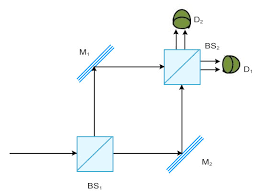
\includegraphics[width=0.5\linewidth]{resources/images/mach-zehnder.png}
        \caption{A Mach-Zehnder interferometer.}
        \label{mach-zehnder}
    \end{figure}
    
    We know that the first beam splitter will cause half of the photons at random to traverse each path. However, superposition can cause photons to travel down \textit{both} paths simultaneously.
    
    Consider sending photons individually into the interferometer. We observe experimentally that interference still occurs at the second beam splitter. Thus, each photon must be interfering \textit{with itself}.
    
    \begin{framedrmk*}[Interference of light]
        It may seem natural that the interference of light should be produced by two photons interfering. However, this cannot be the case! If two photons were to interfere destructively, it would violate the conservation of energy. Similarly, if two photons were to interfere constructively, the amplitude of the electric field would double, but the intensity would quadruple! This shows that light interference can only be the result of quantum superposition.
    \end{framedrmk*}
    
    Thus, a single photon in a Mach-Zehnder interferometer is a superposition of a photon in the upper path and a photon in the lower path.
    
    \begin{framedrmk*} [Superposition as a vector sum]
        A superposition of states can be thought of as the sum of the vectors representing the two states. Note that a vector can be written as the sum of two others in many different ways, and thus a state can be thought of as a superposition of others in many different ways. This will be very helpful later in the semester, as we try to understand states physically. 
    \end{framedrmk*} 
    
    Consider two states $\ket{A}$ and $\ket{B}$, and their superposition $\alpha\ket{A}+\beta\ket{B}$. Suppose a dynamical variable is always measured to be $a$ in state $\ket{A}$ and $b$ in state $\ket{B}$. Then measuring the variable in the superposition yields $a$ with probability proportional to $|\alpha|^2$ and $b$ with probability proportional to $|\beta|^2$. In fact, if $a$ is measured, the state becomes $A$, and the same is true with a measurement of $b$. That is, subsequent measurements will always yield the same result. Note that no \emph{intermediate} results are possible; only one of the two original values. 
    
    \begin{framedexpl}[Polarized photon]
        Consider the example of a photon in Section \ref{polar}. Here the two states are $\ket{\text{photon}:x}$ and $\ket{\text{photon}:y}$, and their superposition is given by $\cos(\alpha)\ket{\text{photon}:x}+\sin(\alpha)\ket{\text{photon}:y}$. The polarizer can be thought of as measuring the polarization of the photon. Then the probability of finding the photon polarized in the $x$ direction is proportional to $|\alpha|^2$, and the probability of finding it polarized in the $y$ direction is proportional to $|\beta|^2$.
    \end{framedexpl}

    We make the necessary physical assumption that superimposing a state with itself does not change any physics: $$\ket{A}\cong 2\ket{A}\cong -\ket{A}\cong i\ket{A}.$$We can see a physical interpretation of this fact using photons.

    \begin{framedexpl}[Polarized photon again]
        Consider a photon polarized in the state $$\alpha\ket{\text{photon}:x}+\beta\ket{\text{photon}:y}.$$This expression has two complex parameters: $\alpha$ and $\beta$. Due to our assumption, however, this state is physically equivalent to the state $$\ket{\text{photon};x}+\frac{\beta}{\alpha}\ket{\text{photon};y}.$$We can thus parameterize a general polarization state of a photon using a single complex parameter $\delta=\frac{\beta}{\alpha}$, or two real parameters. This is indeed physically accurate: a general polarization state of a photon is elliptical, with one variable describing the angle from the $x$-axis and another describing the eccentricity.
    \end{framedexpl}

    \subsection{Spin States}\label{spin_states}

    \textbf{Spin} is an intrinsic property of elementary particles that gives them angular momentum even when they are not rotating or orbiting. We measure spin along the $z$ axis; we find that all matter particles have spin $\frac{1}{2}$ and are either \textbf{spin up} or \textbf{spin down} in the $z$ direction. These are represented by the quantum states $$\ket{\uparrow;z}\text{ and }\ket{\downarrow;z}.$$We can then superimpose these two states to make the state $$\ket{\Psi}=\ket{\uparrow;z}+\ket{\downarrow;z}.$$Given a large number of electrons in this state, measuring the spin in the $z$ direction yields about 50\% spin up measurements and 50\% spin down measurements. 

    \begin{framedrmk*}[Hidden variable theories]
        Einstein believed that 50\% of the electrons are measured to be spin up because they were \textit{already} spin up; some hidden variable determined the spin of the electrons.

        It turns out that in the state $\ket{\Psi}$, 100\% of the electrons are spin up in the $x$ direction while Einstein's ensemble of 50\% spin up electrons and 50\% spin down electrons have the same proportion in the $x$ direction. It has been experimentally measured that all the electrons in the $\ket{\Psi}$ state are spin up in the $x$ direction.  
    \end{framedrmk*}

    \subsection{Entanglement}\label{entanglement}
    
    Consider two non-interacting particles. Suppose particle 1 can be in the states $\ket{u_1}$ and $\ket{u_2}$ and particle 2 can be in the states $\ket{v_1}$ and $\ket{v_2}$. Let the two particles be in the states $\ket{u_1}$ and $\ket{v_1}$, respectively. To represent both these states together, we write $$\ket{u_1}\otimes\ket{v_1}.$$On the other hand, the states of the particles could be more complex. In general, we can have the state $$(\alpha_1\ket{u_1}+\alpha_2\ket{u_2})\otimes(\beta_1\ket{v_1}+\beta_2\ket{v_2}),$$ which we can simply distribute as normal to get $$\alpha_1\beta_1\ket{u_1}\otimes\ket{v_1}+\alpha_2\beta_1\ket{u_2}\otimes\ket{v_1}+\alpha_1\beta_2\ket{u_1}\otimes\ket{v_2}+\alpha_2\beta_2\ket{u_2\otimes\ket{v_2}}.$$

    Now let us consider the following superposition of states: $$\ket{u_1}\otimes\ket{v_1}+\ket{u_2}\otimes\ket{v_2}.$$If this could be written as a product between a state of particle 1 and a state of particle 2, we would need $\alpha_1\beta_1=\alpha_2\beta_2=1$, while $\alpha_1\beta_2=\alpha_2\beta_1=0$. This is impossible; the state above is \textit{unfactorizable}. That is, the state of the first particle is dependent on the state of the second; we say that the particles are \textbf{entangled}.

    \begin{framedexpl}[Spin entanglement]
        Consider 2 spin $\frac{1}{2}$ particles, entangled in the quantum state $$\ket{\uparrow;z}_1\otimes\ket{\downarrow;z}_2+\ket{\downarrow;z}_1\otimes\ket{\uparrow;z}_2.$$
        This state is often used in an allegory with two friends named Alice and Bob, each of whom possesses one of the entangled particles. Even if Alice is several light-years away from Bob, any observation by Bob still instantly determines the state of Alice's particle. It was initially thought that this violated special relativity, which prohibits information from traveling faster than the speed of light. Luckily, it turns out that no information can be transmitted from Bob to Alice, or vice versa, in this way.
    \end{framedexpl}

    \section{Mach-Zehnder Interferometers}

    \subsection{Phase Shifters}
    
    Recall that in a Mach-Zehnder interferometer, a beam of light passes through a beam splitter. Both beams reflect off mirrors and recombine at a second beam splitter, which sends them to two different detectors. Additionally, we can put a device, such as a \textbf{phase shifter}, in between the first beam splitter and one of the mirrors.

    \begin{frameddefn}[Phase shifter]
        A \textbf{phase shifter} multiplies the probability amplitude by a fixed phase factor $\delta\in\mathbb{R}$. If an incoming wave has probability amplitude $\alpha$, the outgoing wave has probability amplitude $\alpha e^{i\delta}$. Since $|\alpha|=|\alpha e^{i\delta}|$, the phase shifter does not change the probability of finding the photon.
    \end{frameddefn}

    \begin{figure}[H]
        \centering
        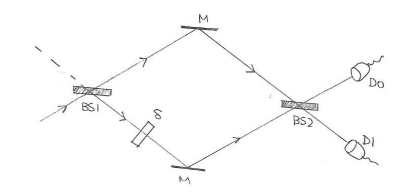
\includegraphics[width=0.7\linewidth]{resources/images/mach-zehnder-phase-shift.png}
        \caption{A Mach-Zehnder interferometer with a phase shifter.}
        \label{mach-zehnder-phase-shifter}
    \end{figure}

    We know that the state of a photon in a Mach-Zehnder interferometer is described by a wavefunction. We express the probability amplitudes of finding the photon in the upper beam and the lower beam by a column vector $\alpha\choose\beta$, where $\alpha,\beta\in\mathbb{C}$ reflect the probabilities of finding the photon in the upper and lower beams, respectively. Furthermore, we \textit{normalize} the probability amplitudes by requiring $|\alpha|^2+|\beta|^2=1$. 
    
    Note that the vector $1\choose0$ represents a photon in the upper beam, and $0\choose 1$ represents a photon in the lower beam. Thus, $\alpha\choose\beta$ is a superposition: ${\alpha\choose\beta} =\alpha {1\choose0}+ \beta {0\choose1}$.

    \subsection{Beam Splitters}

    We now consider the behavior of the beam splitters in detail. Suppose the beam splitter sends photons incident from above (with initial state $1\choose0$) to the state $s\choose t$, and photons incident from below (with initial state $0\choose1$) to the state $u\choose v$. Then we can represent the behavior of the beam splitter in general using linearity: an incident photon in state ${\alpha\choose\beta} =\alpha {1\choose0}+ \beta {0\choose1}$ is sent to the state $$\alpha{s\choose t}+\beta{u\choose v}={\alpha s+\beta u\choose \alpha t+\beta v}=\begin{pmatrix}
      s & u\\ 
      t & v
    \end{pmatrix}{\alpha\choose\beta}.$$Thus, the beam splitter can be completely represented by the 2x2 matrix with entries $s,t,u,$ and $v$, and we will say a beam splitter is equal to its matrix. In practice, the values of the coefficients are determined by the manufacturer. 
    
    \begin{framedrmk*}[Possible beam splitters]
        A beam splitter can be constructed if and only if acting on a normalized photon state always produces a normalized photon state. 
    \end{framedrmk*}
    
    In a \textbf{balanced beam splitter}, the probability that a photon is transmitted is always exactly $\frac{1}{2}$; that is, $|s|^2=|t|^2=|u|^2=|v|^2=\frac{1}{2}$. There are infinitely many complex numbers that satisfy this. However, let's suppose $s=t=u=v=\frac{\sqrt{2}}{2}$ and try acting on the normalized state $\sqrt{2}/{2}\choose \sqrt{2}/{2}$. Carrying out the matrix product yields $1\choose1$, which is not normalized.
    
    What if we instead try setting $v=-\frac{\sqrt{2}}{2}$? Carrying out the product $(\begin{smallmatrix}  s & u\\   t & v\end{smallmatrix}){\alpha\choose\beta}$ gives $\frac{1}{\sqrt{2}}{\alpha+\beta\choose \alpha-\beta}$. Finding the norm of this vector, we see that $$\frac{1}{2}|\alpha+\beta|^2+\frac{1}{2}|\alpha-\beta|^2=\frac{1}{2}[(\alpha+\beta)(\alpha^*+\beta^*)+(\alpha-\beta)(\alpha^*-\beta^*)].$$Note that the $\alpha\beta^*$ and $\beta\alpha^*$ terms vanish! We are left with $$\alpha\alpha^*+\beta\beta^*=|\alpha|^2+|\beta|^2=1.$$Thus, this is a valid balanced beam splitter! In fact, there is more than one possible matrix that satisfies these conditions. Specifically, the beam splitters $$BS_1=\frac{1}{\sqrt{2}}\begin{pmatrix}
      1 & 1\\ 
      1 & -1
    \end{pmatrix},\:\: BS_2=\frac{1}{\sqrt{2}}\begin{pmatrix}
      -1 & 1\\ 
      1 & 1
    \end{pmatrix}$$are both valid.

    \subsection{Experiments}
    
    Suppose we construct a Mach-Zehnder interferometer with these beam splitters: $$BS_1=\frac{1}{\sqrt{2}}\begin{pmatrix}
      1 & 1\\ 
      1 & -1
    \end{pmatrix},\:\: BS_2=\frac{1}{\sqrt{2}}\begin{pmatrix}
      -1 & 1\\ 
      1 & 1
    \end{pmatrix}.$$We send a photon with state $\alpha\choose\beta$ into the device; it passes through both beam splitters in sequence before exiting. Thus, the output state of the photon is $$(BS_2)(BS_1){\alpha\choose\beta}={\beta\choose -\alpha}.$$
    We now perform an experiment. Let us input a photon with state $0\choose1$. Then it should output in the state $1\choose 0$, so it should always hit the upper detector. 
    
    \begin{framedquest*}[What actually happened to the photon?]
        The photon split in the first beam splitter and recombined in the second. From both beams come some complex probability of transmission and reflection. The transmission from the top and reflection from the bottom interfered to give 0, while the transmission from the bottom and reflection from the top interefered to give 1.
    \end{framedquest*}

    Now we perform a slightly different experiment. This time, we place a block of concrete in between the first beam splitter and the bottom mirror. 

    \begin{figure}[H]
        \centering
        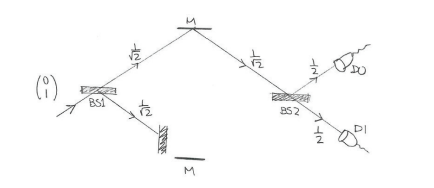
\includegraphics[width=0.7\linewidth]{resources/images/mach-zehnder-concrete.png}
        \caption{A Mach-Zehnder interferometer with a concrete block in the bottom path.}
        \label{mach-zehnder-concrete}
    \end{figure}
    
    We can no longer use the formula above, which was derived assuming both paths were possible. Instead, we must carry out the calculation from scratch. Suppose we send in a photon of state $0\choose 1$. Then the state after the first beam splitter is $$(BS_1){0\choose1}={\frac{1}{\sqrt{2}}\choose\frac{1}{\sqrt{2}}}.$$However, the bottom path is blocked. Thus, the input to the second beam splitter is only the first component: $\frac{1}{\sqrt{2}}\choose0$. Then the output is $$(BS_2){\frac{1}{\sqrt{2}}\choose0}={\frac{1}{2}\choose\frac{1}{2}}.$$There is a 50\% chance that the photon gets blocked, as expected. However, if the photon makes it through, there is a 50/50 chance of observing the photon in the upper or lower detector! Recall that without the concrete block, none of the photons reach the bottom detector.

    \subsection{Elitzur-Vaidman Bombs}
    
    An \textbf{Elitzur-Vaidman bomb} is a bomb triggered by a photon detector tube passing through the bomb. If the detector detects a photon, the bomb explodes. However, if the bomb is defective, the photon is transmitted normally. The question, which was posed by Avshalom Elitzur and Lev Vaidman in 1993, is the following: 

    \begin{framedquest*}[Elitzur-Vaidman bombs]
        Can we decide if an Elitzur-Vaidman bomb is defective without detonating it?
    \end{framedquest*}
    
    This seems obviously impossible, and indeed it is, using classical physics. However, quantum mechanics gives us an unexpected solution by embedding an Elitzur-Vaidman bomb into a Mach-Zehnder Interferometer.
    
    \begin{figure}[H]
        \centering
        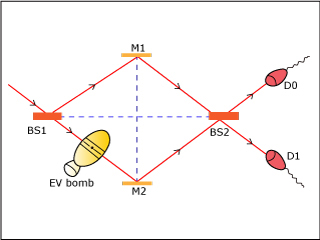
\includegraphics[width=0.5\linewidth]{resources/images/ev-bomb.png}
        \caption{A Mach-Zehnder interferometer with an Elitzur-Vaidman bomb.}
        \label{ev-bomb}
    \end{figure}
    
    We input a photon in the $0\choose1$ state. Suppose the bomb is defective, so the device behaves just like a normal interferometer. Then we can make the following table of possible outcomes and probabilities:

    \begin{center}
        \begin{tabular}{|c|c|}
            \hline
            \textbf{Outcome} & \textbf{Probability} \\
            \hline
            Photon to $D_0$ & 1   \\
            Photon to $D_1$ & 0   \\
            Bomb explodes   & 0   \\
            \hline
        \end{tabular}       
    \end{center}

    On the other hand, suppose the bomb is functional. Then any photon that passes along the bottom path gets absorbed and causes a detonation, so the device behaves like a blocked interferometer. Now our table looks like this:
    
    \begin{center}
        \begin{tabular}{|c|c|}
            \hline
            \textbf{Outcome} & \textbf{Probability} \\
            \hline
            Photon to $D_0$ & $1/4$   \\
            Photon to $D_1$ & $1/4$  \\
            Bomb explodes   & $1/2$  \\
            \hline
        \end{tabular}       
    \end{center}
    
    Note that $\frac{1}{4}$ of the time with a functional bomb, the photon is observed by $D_1$, whereas this never happens with a defective bomb! Thus, if we observe a photon at $D_1$, we know the bomb works without denotating it!
    
    \begin{framedrmk*}[Improvements]
       Is a $50\%$ chance that your lab explodes too high? It's been experimentally proven that this setup can be improved to decrease the probability of detonation arbitrarily low.
    \end{framedrmk*}

    \chapter{Matter Waves}
    \section{Particle-Wave Duality}\label{particle_wave_duality}
\subsection{The Photoelectric Effect}\label{photoelectric}

The \textbf{photoelectric effect} was observed by Hertz in 1887. He found that polished metal plates, when irradiated, may emit electrons. These electrons are called \textbf{photoelectrons} and form a \textbf{photoelectric current}.

There is a threshold frequency $\nu_0$ such that a photoelectric current exists only when irradiated with light with frequency $\nu>\nu_0$. ($\nu_0$ is extremely hard to calculate. It depends on the type of metal and the configuration of atoms at the surface.)

Furthermore, Hertz found that the magnitude of the photoelectric current is proportional to the intensity of the light. On the other hand, the energy of each photoelectron is independent of the light intensity. Later, it was found that the energy of the photoelectrons is proportional to the \textit{frequency} of the light.

In 1905, Einstein proposed that light is composed of quanta (photons) with energy $E=h\nu$.

\begin{framedrmk*}[Planck's constant]
   Planck introduced his constant $h$ when trying to find the relationship between the intensity of light radiated by a blackbody and the frequency of the light. 
\end{framedrmk*}

Einstein also theorized that the electrons in metal plates begin in some negative potential of height $W$, the \textbf{work function}. Here, $W$ is the energy needed to release an electron from the potential. If he was right, then the energy of the electron $E_{e^-}$ and the energy of the incident photon $E_{\gamma}$ would have to obey the relation $$E_{e^-}\approx\frac{1}{2}mv^2=E_{\gamma}-W=h\nu-W.$$This result was verified experimentally by Millikan in 1915, who also measured the value of $h$ to within $1\%$.

\begin{framedquest}[Photoelectric effect]
    We shine UV light with wavelength $\lambda=290\,\text{nm}$ on a metal with $W=4.05\,\text{eV}$. What are the energy $E_{e^-}$ and speed $v$ of the electrons?
\end{framedquest} 

\begin{framedansw}
    We begin by finding the energy of the photon: $E_{\gamma}=h\nu=\frac{hc}{\lambda}=\frac{2\pi\hbar c}{\lambda}$. Thus, we have $$E_{\gamma}=\frac{2\pi(197)\times 10^{-15}}{290\times 10^{-9}}\approx 4.28 eV.$$We therefore have $E_{e^-}=E_{\gamma}-W=0.23\,\text{eV}$. This is small enough that the electron is non-relativistic, so we have $0.23\,\text{eV}=\frac{1}{2}m_ev^2=\frac{1}{2}m_ec^2\frac{v^2}{c^2}$. Since the rest energy of an electron is around half a million electron volts, we have $0.23\approx\frac{1}{2}(511000\,\text{eV})(\frac{v}{c})^2$. From here, we can solve for $v$.
\end{framedansw}

\begin{framedtip*}[A nice number]
    The value $\hbar c$ is about $197.33\approx 200\,\text{MeV} \cdot \text{fm}$. 
\end{framedtip*}

\subsection{Planck's Constant \& Compton Wavelength} \label{compton_wavelength}

Planck's constant $h$ is an extremely important quantity! Consider the equation $E=h\nu$. Since we know the units of $E$ and $\nu$, we can solve for the units of $h$:\footnote{The square brackets above indicate the \textit{units} of their arguments. For example, $[p]$ represents the units of momentum, or $M\cdot\frac{L}{T}$.} $$[h]=\frac{M\frac{L^2}{T^2}}{\frac{1}{T}}=\frac{ML^2}{T}.$$

This tells us the units of $h$, but it would be more helpful to find a familiar physical quantity with the same units. We can rearrange the above equation to see $$[h]=L\cdot M\frac{L}{T}=[r][p]=[J].$$Thus, $h$ has units of angular momentum! Knowing this allows us to construct other fundamental quantities. For example, given a particle with momentum $p$, we can construct a length by taking the quantity $\frac{h}{p}$. In fact, this is called the \textbf{de Broglie wavelength} of the particle. 

Even if the particle is at rest, we can still construct an associated length by taking the quantity $\frac{h}{mc}$, as $c$ is a fundamental quantity with units of velocity. This value is called the \textbf{Compton wavelength} of the particle and is denoted $l_c(m)$. 

Why is this (seemingly arbitrary) quantity important? Consider a particle at rest with mass $m$ and rest energy $mc^2$. What is the wavelength of a photon with the same energy as the particle?

We can calculate the wavelength $\lambda$ by the relation $mc^2=E_{\gamma}=\frac{hc}{\lambda}$. Solving, we see $\lambda=\frac{h}{mc}$, or the Compton wavelength of the particle! This provides a physical interpretation of the Compton wavelength.

\begin{framedrmk*}[Experimental effects]
    In quantum field theory, shining light with the Compton wavelength of an electron onto an electron can create new particles. This makes it difficult to find the position of a particle to an uncertainty smaller than its Compton wavelength, as new particles can be spontaneously created or destroyed at these scales.
\end{framedrmk*}

\begin{framedquest}[Compton wavelength of an electron]
    What is the Compton wavelength of an electron?
\end{framedquest}

\begin{framedansw}
    We have $$l_c(m_e)=\frac{h}{m_ec}=\frac{2\pi\hbar c}{m_ec^2}\approx 2426\, \text{fm}=2.426\,\text{pm}.$$The picometer is a natural unit for atomic calculations; the Bohr radius is about $50\,\text{pm}$.
\end{framedansw}

\subsection{Compton Scattering}
\label{compton_scattering}

Arthur Compton, the namesake of the Compton wavelength, conducted experiments shining high-energy x-rays on atoms. Since the x-ray energy dominates the binding energy of the electrons, this is almost like shining x-rays on free electrons. \textbf{Compton scattering} is high-energy photons scattering on ``virtually'' free electrons. 

Compton's results contradicted the classical model of \textbf{Thomson scattering}, which treats photon scattering as the radiation produced by an electron in an incident electromagnetic wave. The electric field of the wave shakes the electron, causing it to oscillate, and the radiated field has the same frequency as the incoming electromagnetic wave. In Thomson scattering, the differential scattering cross-section at angle $\theta$ is given by\footnote{Here, $\sigma$ is the area of a part of the incident beam that possesses the right energy to scatter at angle $\theta$. Basically, the right-hand side is a plot of intensity with respect to angle $\theta$. More information about cross-sections can be found \href{https://www.sciencedirect.com/topics/engineering/scattering-cross-section}{here}.} $$\frac{d\sigma}{d\Omega}=(\frac{e^2}{mc^2})^2\frac{1}{2}(1+\cos^2\theta).$$

Compton found that Thomson scattering is not accurate at high energies. To correct it, we must treat a photon as a particle with some energy $E_\gamma=h\nu$ and momentum $p_\gamma=\frac{h}{\lambda}$ colliding with an electron.\footnote{These expressions come from Einstein's famous relation $$E^2-p^2c^2=m^2c^4.$$ Since photons are massless, the equation reduces to $E_\gamma=p_\gamma c$. We also know $E_\gamma=h\nu$, so $p_\gamma=\frac{E_\gamma}{c}=\frac{h\nu}{c}=\frac{h}{\lambda}$.} 

There are two fundamental facts about this scattering. First, the photon cannot be completely absorbed by the electron, which can be shown using a relativistic calculation. Additionally, the electron gains kinetic energy from the collision, so the photon must lose energy. Therefore, the final wavelength $\lambda_f$ must be larger than the initial wavelength $\lambda_i$. In fact, we can compute that $$\lambda_f=\lambda_i+l_c(m_e)(1-\cos\theta).$$Here, $l_c(m_e)$ is the Compton wavelength of the electron. We see that $\lambda_i\leq \lambda_f\leq 2\lambda_i$.

In his experiment, Compton used Molybdenum x-rays with a wavelength of $\lambda_i=0.0709\,\text{nm}$, corresponding to a photon energy of $E_{\gamma}=17.49\,\text{keV}$. He shined the x-ray beam on a carbon foil target and observed the relationship between intensity and wavelength at various angles. In particular, at $\theta=90^\circ$, he observed the following plot.

\begin{figure}[H]
    \centering
    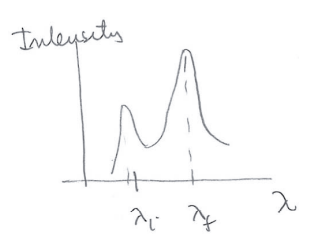
\includegraphics[width=0.5\linewidth]{resources/images/compton-scattering.png}
    \caption{Compton's results at $\theta=90^\circ$.}
    \label{compton-scattering}
\end{figure}

The observed value of $\lambda_f$ is around $0.0731\,\text{nm}$, which aligns quite well with the expected value $\lambda_f=\lambda_i+l_c(m_e)$, where $l_c(m_e)\approx 0.0024\,\text{nm}$. So the second peak makes sense, but how can we interpret the first peak? It represents a process in which the electron remains bound after collision with the photon. Then the entire atom recoils, so the relevant Compton wavelength is that of the atom, which is negligible. Thus, there is no detectable change in the wavelength of the photon.

\subsection{De Broglie's Proposal}
\label{deBroglie_proposal}

By 1924, the wave nature and particle nature of the photon were both certain, but the resolution of how to combine them was unclearly. In that year, Louis de Broglie had the great insight that the photon has a \textbf{particle-wave duality}: both descriptions are required to fully capture its behavior. In fact, he further proposed that \textit{all} matter particles also behave as waves, and that all waves have particle properties. In fact, from Section \ref{schrodinger}, we know that the wave is a \textit{probability wave}. 

Consider a photon. As a particle, it has energy and momentum, and as a wave, it has frequency. This effect is universal; all matter particles have associated \textbf{matter waves}, which represent probability amplitudes. Specifically, for a particle of momentum $p$, we associate with it a plane wave with wavelength $\lambda=\frac{h}{p}$, which is the de Broglie wavelength from Section \ref{compton_wavelength}. This has been experimentally verified by performing the double-slit experiment on increasingly large particles. In fact, we have now performed such experiments on molecules with masses of $10,000$ atomic mass units and de Broglie wavelengths of $1\,pm$. 

\section{Matter Waves \& de Broglie Wavelength}
\label{matter_waves_deBroglie_wavelength}

\subsection{De Broglie Wavelength in Different Frames}
\label{debroglie_in_different_frames}

As we discussed above, de Broglie postulated that a free particle with momentum $p$ can be associated with a plane (matter) wave with wavelength $\lambda=\frac{h}{p}$. Eventually, this wave would become the wavefunction, and the equations describing it would become the Schrödinger equation. In the simplest case, there is only one complex wavefunction $\Psi(\vec{x},\,t)$.

Let's examine the formula $\lambda=\frac{h}{p}$ in more detail. Then $p=\frac{h}{\lambda}=(\frac{h}{2\pi})(\frac{2\pi}{\lambda})=\hbar k$. Consider two non-relativistic observers with rest frames $S$ and $S'$ moving with velocity $+v$ in the $x$-direction relative to $S$. 

Let the particle have mass $m$, velocity $u$ in frame $S$, and velocity $u'$ in frame $S'$. Let its momentum be $p=mu$ in frame $S$ and $p'=mu'$ in frame $S'$. The coordinates are easily related by Galilean transformations: $$x'=x-vt,\;t'=t.$$Then $\frac{dx'}{dt'}=\frac{dx}{dt}-v$. Thus, $u'=u-v$. Similarly, $p'=p-mv$. Therefore, $$\lambda'=\frac{h}{p-mv}\neq\lambda=\frac{h}{p}.$$Thus, the de Broglie wavelength of a particle is dependent on the frame of reference. On the other hand, consider any \textit{measurable} wave. For a general wave, the crucial value is the \textbf{phase} $\phi=kx-\omega t$. The wave itself can be represented as some function of $\phi$. For any point on the wave, all observers will agree on the phase at the point; for this reason, we call the phase a \textbf{Galilean invariant}.

We can rewrite the phase as $$\phi=k(x-\frac{\omega}{k}t)=\frac{2\pi}{\lambda}(x-vt)=\frac{2\pi}{\lambda}x-\frac{2\pi v}{\lambda}t.$$From this expression we see that $k=\frac{2\pi}{\lambda}$ and $\omega=\frac{2\pi v}{\lambda}$. 

\begin{framedtip*}[$k$ and $\omega$]
   Given an expression for the phase of a wave, we can read the wavenumber $k$ and the frequency $\omega$ as the coefficients of $x$ and $t$, respectively. 
\end{framedtip*}

Since phase is a Galilean invariant, we must have $\phi'=\phi$ for all frames $S'$ and $S$. For the same Galilean transformation as above, we have $x=x'+ut'$ and $t=t'$. Thus, $$\frac{2\pi}{\lambda}(x-vt)=\frac{2\pi}{\lambda}(x'+ut'-vt')=\frac{2\pi}{\lambda}x'-\frac{2\pi v}{\lambda}(1-\frac{u}{v})t'.$$Since $k'$ and $\omega'$ are the coefficients of $x'$ and $t'$, respectively, we have $k'=k$ and $\omega'=\omega(1-\frac{u}{v})$. Importantly, since the wavenumber does not change, we must also have $\lambda'=\lambda$. 

We conclude that the wavefunction $\Psi$ is \textit{not} directly measurable, as any directly measurable wave must obey the Galilean invariance above. Additionally, we have found that $\Psi$ is not Galilean invariant: two observers may disagree on the wavefunction at a point in time. That is, for some point measured by two observers as $(x,t)$ and $(x',t')$, we may have $\Psi(x,t)\neq\Psi'(x',t')$. 

\subsection{Frequency of a Matter Wave}
\label{freq_matter_waves}

We have established that a particle with momentum $p$ can be associated with a matter wave of wavenumber $k$ such that $p=\hbar k$. In fact, if the particle has energy $E$, the frequency of the matter wave satisfies $E=\hbar\omega$. These two equations are incredibly important and are together called the \textbf{de Broglie relations}: \begin{align*} \begin{split}
    p&=\hbar k, \\ E&=\hbar\omega.    
\end{split}\tag{de Broglie relations}
\end{align*}

The de Broglie relations on $p$, $k$, $E$, and $\omega$ are fundamental \textit{postulates} of quantum mechanics. That means we cannot derive these relations, but we can test them in specific cases and show that they align with our expectations. Here, we will discuss three pieces of evidence supporting the de Broglie relations. 

\textbf{1. Phase and Group Velocity}

Consider a matter wave with phase $\phi=kx-\omega t$, and assume the de Broglie relations hold. Then the \textbf{phase velocity} $v_p=\frac{\omega}{k}$ of the wave is given by $$v_p=\frac{\omega}{k}=\frac{E}{p}=\frac{\frac{1}{2}mv^2}{mv}=\frac{1}{2}v.$$
Additionally, we define the \textbf{group velocity} $v_g=\frac{d\omega}{dk}$, given by $$v_g=\frac{d\omega}{dk}\bigg|_k=\frac{dE}{dp}=\frac{d}{dp}(\frac{p^2}{2m})=\frac{p}{m}=v.$$
Notice that the phase velocity, which is the speed of a \textit{single wave crest} through the medium, is half the velocity of the particle. When the phase velocity is constant, as in a sine wave, we have a \textbf{plane wave}. Plane waves cannot carry any information, so a particle cannot be represented by a plane wave. Instead, it must be represented by a \textbf{wavepacket}, which we will discuss soon. For this reason, the phase velocity is not very meaningful.

On the other hand, the group velocity, which represents the speed of the \textit{wavepacket}, perfectly equals the speed of the particle. In fact, $v_g=v$ even for relativistic particles. Thus, the de Broglie relations cause matter waves to move with the same speed as particles, which is evidence that they are true.

\textbf{2. Four-Vectors}

If you happen to have studied special relativity, you will recall that the four-momentum is defined as $\vec{P}=(\frac{E}{c},\,\vec{p})$ (if not, don't worry --- this is the only relativity in this course!). Similarly, for a wave whose phase is relativistically invariant, $(\frac{\omega}{c},\,k)$  is also a four-vector. Then both de Broglie relations follow from equating two four-vectors: $$(\frac{E}{c},\,\vec{p})=\hbar(\frac{\omega}{c},\,\vec{k}).$$ This supports the de Broglie relations because they would then be true in all Lorentz frames. In other words, this shows that the de Broglie relations are consistent relativistically.

\textbf{3. Photons}

For photons, the de Broglie relations agree with Einstein's energy quanta: $E_\gamma=h\nu=\hbar\omega.$ In the footnote on page 16, we saw that photons also have momentum $p_\gamma=\frac{\hbar}{\lambda}=\hbar k$. We can therefore think of the de Broglie relations as simply extending Einstein's findings for photons to matter particles.

\section{Wavepackets}
\label{wavepackets}
\subsection{Stationary Phase Approximation}
\label{stationary_phase_approximation}

Suppose we have some function of frequency in terms of wavenumber $\omega(k)$. As defined in Section \ref{freq_matter_waves}, the group velocity is $v_g=\frac{d\omega}{dk}$ and represents the velocity of a ``packet'' constructed by superimposing waves. Figure \ref{wavepacket} shows a screenshot of a wavepacket, its sinusoidal wave components, and the component amplitudes.\footnote{This screenshot is from the PhET \href{https://phet.colorado.edu/en/simulations/fourier-making-waves} {\textit{Fourier: Making Waves \emph{simulation}}}. The PhET interactive simulations are excellent resources created by the University of Colorado.}

\begin{figure}[H]
    \centering
    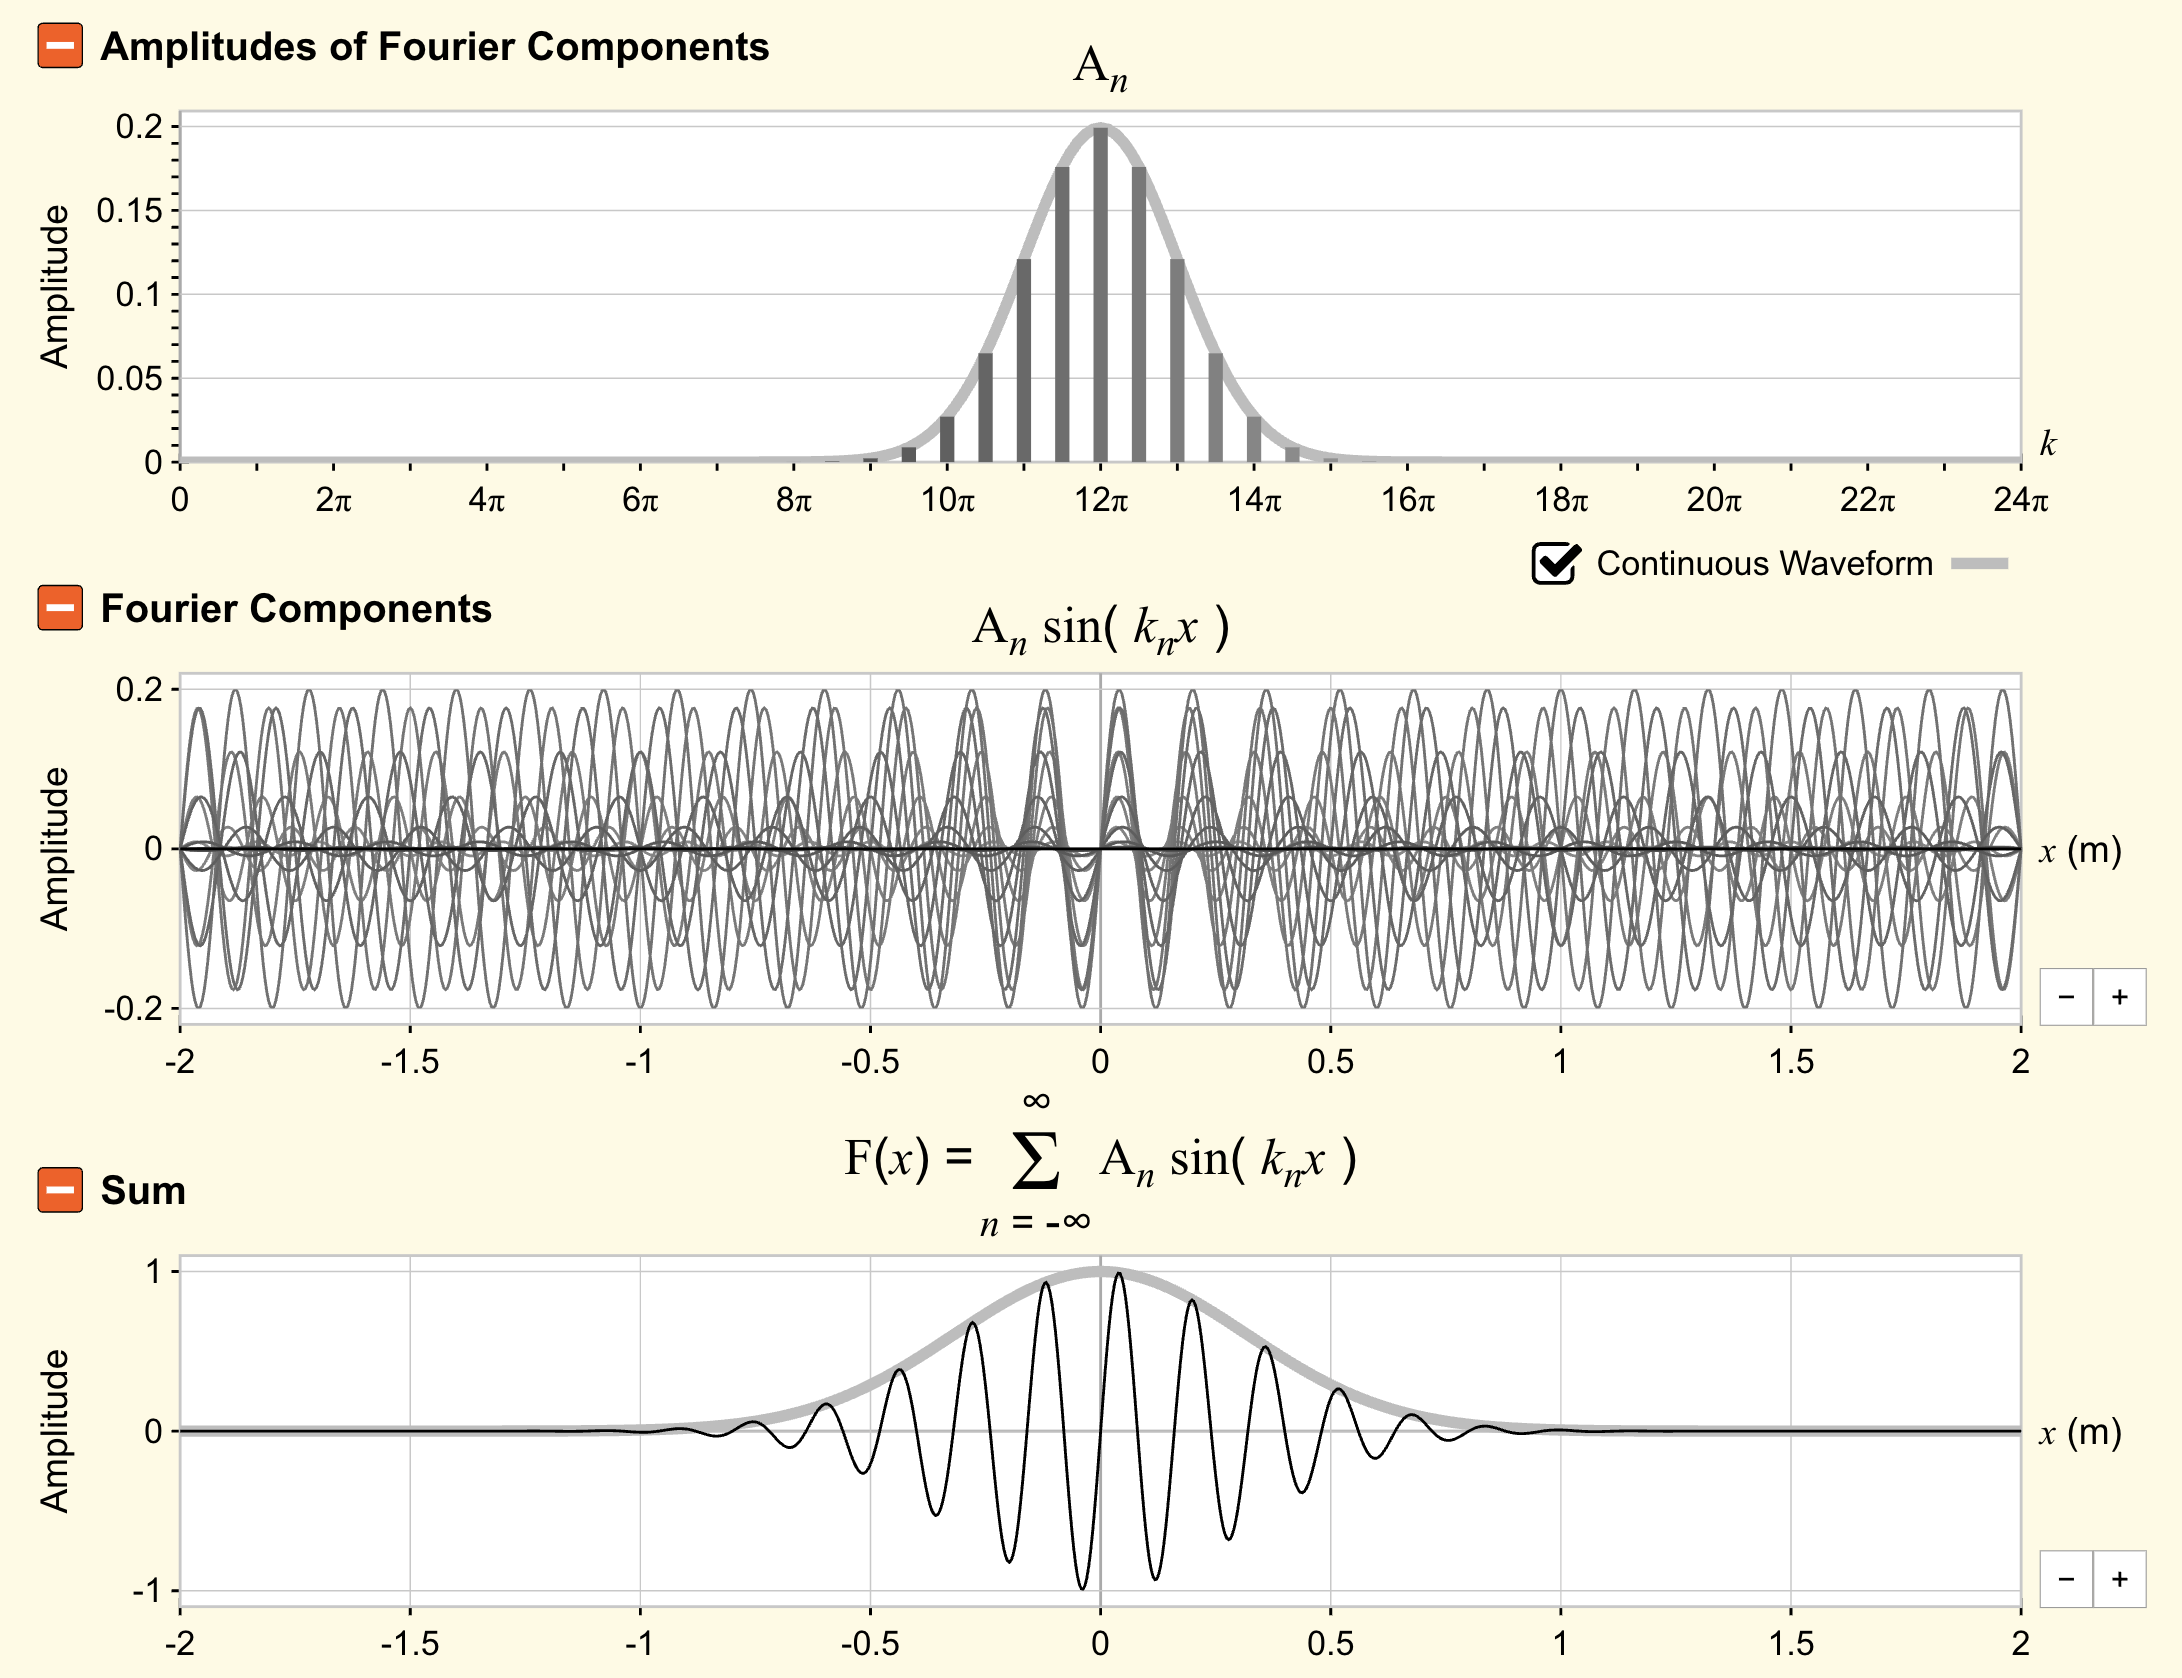
\includegraphics[width=0.8\linewidth]{resources/images/wavepacket.png}
    \caption{Top to bottom: a graph of the amplitudes of the component waves ($\Phi(k)$ below), a graph of the component waves ($\Phi(k)e^{i\phi(k)}$), and a graph of the wavepacket ($\int dk\,\Phi(k)e^{i\phi(k)}$).}
    \label{wavepacket}
\end{figure}
Consider the general wavefunction representing the superposition of infinitely many waves of phase $\phi(k)=kx-\omega(k)t$ and amplitude $\Phi(k)$:$$\Psi(x,\,t)=\int dk\;\Phi(k)e^{i\phi(k)}.$$We also assume that $\Phi(k)$ is both real and 0 almost everywhere, except for a narrow peak around a value $k_0$. In Figure \ref{wavepacket}, $k_0=12\pi$. We would like to see how the wavefunction behaves over time. There is a quick way of seeing this, called the \textbf{principle of stationary phase}, or the stationary phase approximation. 

\begin{framedthm}[Principle of stationary phase]\label{principle_stationary_phase}
    The integral of a function $f(x)$ multiplied by some rapidly oscillating value like $\sin(\phi(x))$ will be approximately 0 except in places with small oscillating frequency. 
\end{framedthm}

Here, the function is $\Phi(k)$ and the oscillating value is $e^{i\phi(k)}$. Since the integral only has a chance to be nonzero at $k\approx k_0$ where $\Phi(k)\neq 0$, the phase must be stationary with respect to $k$ at this point. And since we assumed $\Phi(k)$ to be real, the phase is only contributed by $\phi(k)=kx-\omega(k)t$. Thus, we must have $$\frac{d\phi(k)}{dk}\bigg|_{k_0}=x-\frac{d\omega(k)}{dk}\bigg|_{k_0}t=0.$$Then we need $\frac{d\omega(k)}{dt}=\frac{x}{t}$, which confirms that the group velocity $v_g=\frac{d\omega(k)}{dt}$ is indeed the speed of the wavepacket.

\subsection{Group Velocity}\label{group_velocity}

We can also show this result without approximating. We rewrite the wavefunction $$\Psi(x,\,t)=\int dk\;\Phi(k)e^{i(kx-\omega(k) t)}.$$At time $t=0$, we have $$\Psi(x,\,0)=\int dk\;\Phi(k)e^{ikx}.$$Since the integral is only nonzero for $k\approx k_0$, we linearly approximate $\omega(k)$ as $$\omega(k)= \omega(k_0)+ (k-k_0)\frac{d\omega(k)}{dt}\bigg|_{k_0}+O((k-k_0)^2).$$Substituting back into the integral, $$\Psi(x,\,t)=\int dk\;\Phi(k)\,e^{ikx}\,e^{-i\omega(k_0) t}\,e^{-ik\frac{d\omega}{dk}|{k_0}t}\,e^{ik_0\frac{d\omega}{dk}|_{k_0}t}.$$ Our integral is now looking pretty bad. However, note that the second and fourth exponential factors are independent of $k$! We can take these out of the integral to get $$\Psi(x,\,t)=e^{-i\omega(k_0) t}\,e^{ik_0\frac{d\omega}{dk}|_{k_0}t}\int dk\;\Phi(k)\,e^{ik(x-\frac{d\omega}{dk}|{k_0}t)}.$$The integral can now be written in terms of the wavefunction at time 0. Taking the magnitude of both sides to remove the annoying exponential phases outside the integral, we see that $$|\Psi(x,\,t)|=|\Psi(x-\frac{d\omega}{dk}\bigg|_{k_0}t,\,0)|.$$Just as in Section \ref{stationary_phase_approximation}, we see that the wavepacket moves with speed given by the group velocity $v_g= \frac{d\omega}{dk}|_{k_0}$.


    \chapter{Operators \& the Schrödinger Equation}    \section{Operators}
\label{operators}
\subsection{Wave of a Free Particle}
\label{free_particle}

Consider a particle with energy $E$ and momentum $p$, whose matter wave has wavelength $\omega$ and wave number $k$ given by $E=\hbar\omega$ and $p=\hbar k$. Suppose the particle moves in the positive $x$-direction. The matter waves are combinations of plane waves, of which there are a few possibilities:

\begin{enumerate}
    \item $\sin(kx-\omega t)$
    \item $\cos(kx-\omega t)$
    \item $e^{i(kx-\omega t)}$
    \item $e^{i(-kx+\omega t)}$
\end{enumerate}

We will now determine the specific shape of the matter wave. The argument will rely on superposition (Section \ref{superposition}) and a vague notion of probability. In particular, we will build a wave that has equal probability of moving to the right or to the left, using each of the possible plane waves above, and show that two of these waves are unphysical.

\begin{enumerate}
    \item $\Psi(x,\,t)=\sin(kx-\omega t)+\sin(kx+\omega t)=2\sin(kx)\cos(\omega t)$. This is unacceptable, since it vanishes for all $x$ at times $t=\frac{\pi}{2\omega},\,\frac{3\pi}{2\omega},\,\frac{5\pi}{2\omega}\ldots$, which means the particle would suddenly disappear at these times.
    \item $\Psi(x,\,t)=\cos(kx-\omega t)+\cos(kx+\omega t)=2\cos(kx)\cos(\omega t)$. This is no good for the same reason as 1.
    \item $\Psi(x,\,t)=e^{i(kx-\omega t)}+e^{i(-kx-\omega t)}=(e^{ikx}+e^{-ikx})e^{-i\omega t}=2\cos(kx)e^{-i\omega t}$. Since $e^{i\omega t}\neq 0$, this wave never disappears for all $x$.  
    \item $\Psi(x,\,t)=e^{i(-kx+\omega t)}+e^{i(kx+\omega t)}=2\cos(kx)e^{i\omega t}$. This wave is just as good as 3.
\end{enumerate}

We have two remaining possibilities for the wavefunction, given by 3. and 4. Suppose they were both valid. Then we could superimpose them to get the wavefunction of a rightward-moving particle, $$\Psi(x,\,t)=e^{i(kx-\omega t)}+e^{i(-kx+\omega t)}=2\cos(kx-\omega t).$$However, this is equivalent to 2., which we have shown is not a possible candidate for a wavefunction. Therefore, we must choose between 3. and 4. By convention, physicists choose 3.

\begin{frameddefn}[Matter wave of a free particle]\label{free_particle_wave}
    The matter wave or wavefunction of a free particle with $p=\hbar k$ and $E=\hbar\omega$ is given by $$\Psi(x,\,t)=e^{ikx-i\omega t}.$$In three dimensions, we have $\vec{p}=\hbar\vec{k}$ and the wavefunction is $$\Psi(x,\,t)=e^{i\vec{k}\vec{x}-i\omega t}.$$
\end{frameddefn}

We will now use Definition \ref{free_particle_wave} to derive the expression governing \textit{all} wavefunctions.

\subsection{Momentum Operator}\label{p_operator}

Suppose we would like to find the momentum of the particle above, given its wavefunction. Note that $$\frac{\hbar}{i}\frac{\partial}{\partial\,x}\Psi(x,\,t)=\hbar k\Psi(x,\,t)=p\Psi(x,\,t).$$We define $\frac{\hbar}{i}\frac{\partial}{\partial x}$ to be the \textbf{momentum operator} $\hat{p}$, meaning that it multiplies a wavefunction $\Psi$ by its momentum $p$. That is, $$\hat{p}\Psi(x,\,t)=p\Psi(x,\,t).$$ Recall that in linear algebra, an \textbf{eigenvector} of a matrix $A$ is a vector $v$ such that $A\vec{v}=k\vec{v}$ for some \textbf{eigenvalue} $k$. Similarly, we call $\Psi(x,\,t)$ an \textbf{eigenstate} or \textbf{eigenfunction} of $\hat{p}$ with eigenvalue $p$. In general, operators behave like matrices and wavefunctions behave like vectors. In more advanced treatments of quantum mechanics, it can be shown that all operators can be represented by $2\times 2$ matrices.

Note that $\Psi(x,\,t)$ is a state of \textit{definite momentum}; given $\Psi$, we can find $p$ exactly. This makes sense, since we defined $\Psi$ for a particle with momentum $p$. As we will see later, not all wavefunctions have definite momentum.

\subsection{Energy Operator}\label{e_operator}

Now let's find the \textbf{energy operator} in a similar way --- this will be an expression that produces $E\Psi=\hbar\omega\Psi$ when acting on $\Psi$. We can write $$i\hbar\frac{\partial}{\partial t}\Psi(x,\,t)=i\hbar(-i\omega)\,\Psi(x,\,t)=E\,\Psi(x,\,t).$$Note that nowhere in the above two derivations did we use the physical knowledge that $E=\frac{p^2}{2m}$. Thus, instead of taking the energy operator to be $i\hbar\frac{\partial}{\partial t}$, suppose we have some arbitrary operator $\mathcal{O}$ such that $\mathcal{O}\Psi=E\Psi$. We have $$\mathcal{O}\Psi=\frac{p^2}{2m}\Psi=\frac{p}{2m}(p\,\Psi)=\frac{p}{2m}\frac{\hbar}{i}\frac{\partial}{\partial x}\Psi.$$Since $p$ is a constant, it can be moved into the derivative. Thus, $$\mathcal{O}\,\Psi=\frac{1}{2m}\frac{\hbar}{i}\frac{\partial}{\partial x}(\frac{\hbar}{i}\frac{\partial}{\partial x}\Psi).$$Rearranging, we see that $$\mathcal{O}\,\Psi=E\,\Psi=-\frac{\hbar^2}{2m}\frac{\partial^2}{\partial x^2}\Psi.$$From this we read off the energy operator $\hat{E}=-\frac{\hbar^2}{2m}\frac{\partial^2}{\partial x^2}$, such that $\hat{E}\Psi=E\Psi$. As above, we call $\Psi$ an eigenstate of the energy operator with eigenvalue $E$. Note that this yields a nice analog of the classical law, $$\hat{E}=\frac{\hat{p}^2}{2m}.$$However, recall that we also had $E\Psi=i\hbar\frac{\partial}{\partial\,t}\Psi$. When applied to free particles, the Schrödinger equation, which we first encountered back in Section \ref{schrodinger}, simply equates these two definitions of the energy operator:
\begin{Dequation}
    \begin{align*}
        i\hbar\frac{\partial}{\partial t}\Psi=-\frac{\hbar^2}{2m}\frac{\partial^2}{\partial x^2}\Psi. \tag{Schrödinger equation}
    \end{align*}
\end{Dequation}
Strictly speaking, this is the \textit{free-particle} Schrödinger equation; the \textit{general} Schrödinger equation takes into account potential energy, which we will see soon.

\subsection{Commutators}\label{commutators}

Notice that operators can be as simple as scalar products --- the number $3$, for example, can be considered as an operator that triples its argument. We introduce an operator $\hat{x}$, which, acting on a function of $x$, multiplies it by $x$. That is, $\hat{x}f(x)=xf(x)$. We mentioned before that operators are represented by matrices. Recall that matrix multiplication is non-commutative. We thus want to know if \textit{operators} commute.

\begin{framedrmk*}[Heisenberg's path to quantum]
    While Schrödinger formulated quantum mechanics beginning with wave mechanics and the Schrödinger Equation, Heisenberg started with operators and matrices. Later, Schrödinger showed that the two approaches were equivalent.
\end{framedrmk*}

We wish to know if the operators $\hat{x}$ and $\hat{p}$ commute. That is, for some arbitrary function $\phi(x,\,t)$, $$\text{Does}\;\ \hat{x}\hat{p}\phi-\hat{p}\hat{x}\phi=0?$$We have \begin{align*}
\hat{x}\hat{p}\phi-\hat{p}\hat{x}\phi&=\hat{x}(\hat{p}\phi)-\hat{p}(\hat{x}\phi)\\&=\hat{x}(\frac{\hbar}{i}\frac{\partial \phi}{\partial x})-\hat{p}(x\phi)\\&=\frac{\hbar}{i}x\frac{\partial\phi}{\partial x}-\frac{\hbar}{i}\frac{\partial}{\partial x}(x\phi).
\end{align*}Note that applying the product rule to the second term, we see that $\frac{\partial}{\partial x}(x\phi)=x\frac{\partial\phi}{\partial x}+\phi$.  The first term cancels, so we see that $$\hat{x}\hat{p}\phi-\hat{p}\hat{x}\phi=-\frac{\hbar}{i}\phi=i\hbar\phi.$$Since operators, like matrices, distribute, we have $(\hat{x}\hat{p}-\hat{p}\hat{x})\phi=i\hbar\phi$. Notice that $\hat{x}\hat{p}-\hat{p}\hat{x}$ is an operator that, when applied to a function $\phi$, multiplies $\phi$ by $i\hbar$. Since we can treat numbers as operators, we can write the operator equation $$\hat{x}\hat{p}-\hat{p}\hat{x}=i\hbar.$$We define the \textbf{commutator} of two operators $\hat{A}$ and $\hat{B}$ to be $[\hat{A},\,\hat{B}]=\hat{A}\hat{B}-\hat{B}\hat{A}.$

\begin{frameddefn}[Commutator]
    The \textbf{commutator} of two operators $\hat{A}$ and $\hat{B}$ is $$[\hat{A},\,\hat{B}]=\hat{A}\hat{B}-\hat{B}\hat{A}.$$
\end{frameddefn}

Thus, we can write $$[\hat{x},\,\hat{p}]=i\hbar.$$
Importantly, this is nonzero, which means the $\hat{x}$ and $\hat{p}$ operators do \textit{not} commute. This is the basis of the uncertainty principle, as we will see later.

\section{The Schrödinger Equation}\label{schrodinger_main}

\subsection{Free-Particle Schrödinger Equation}\label{free_particle_schrodinger}

Let's input the plane wavefunction $\Psi=e^{ikx-i\omega t}$ to the free-particle Schrödinger Equation from Section \ref{e_operator}, $$i\hbar\frac{\partial}{\partial t}\Psi=-\frac{\hbar^2}{2m}\frac{\partial^2}{\partial x^2}\Psi.$$We get \begin{align*}
i\hbar(-i\omega)\Psi&=-\frac{\hbar^2}{2m}(ik)^2\Psi \\
\implies\hbar\omega&=\frac{(\hbar k)^2}{2m}\\
 \implies E&=\frac{p^2}{2m}.
\end{align*}
Thus, the free-particle Schrödinger Equation directly yields the classical relationship between energy and momentum. 

As mentioned in Section \ref{stationary_phase_approximation}, the general solution to the free-particle Schrödinger equation can be written as the superposition of infinitely many wavefunctins: $$\Psi(x,\,t)=\int_{\infty}^{\infty}dk\;\Phi(k)\,e^{ikx-i\omega(k)t}.$$In Section \ref{group_velocity}, we proved that if $\Phi(k)$ is localized around some $k_0$, the group velocity $\frac{d\omega}{dk}$ must be given by $$v_g=\frac{dE}{dp}=\frac{p}{m}=v.$$

\subsection{General Schrödinger Equation}
\label{general_schrodinger}

Recall that we can write the free-particle Schrödinger equation in the form $$i\hbar \frac{\partial\Psi}{\partial t}=\hat{E}\,\Psi,$$where $\hat{E}=\frac{\hat{p}^2}{2m}$.
Now consider a particle whose potential energy is given by a function $V(x,\,t)$. We call $V$ the \textbf{potential} of the particle. Then the total energy is the sum of the kinetic and potential energies, so $$\hat{E}=\frac{\hat{p}^2}{2m}+V(x,\,t).$$We call the total energy operator the \textbf{Hamiltonian operator} $\hat{H}=\hat{E}$. Then the Schrödinger equation takes the following form, which is true in general: 

\begin{framedthm}[General Schrödinger Equation]\label{general_schrodinger_eqn}
    $$i\hbar\frac{\partial\Psi}{\partial t}=\bigg(-\frac{\hbar^2}{2m}\frac{\partial^2}{\partial x^2}+V(x,\,t)\bigg)\Psi.$$
\end{framedthm}

In Theorem \ref{general_schrodinger_eqn}, $V(x,t)$ should be thought of as a numerical operator that multiplies $\Psi$ by a scalar value. 

\begin{framedtip*}[Hamiltonian operators]
    A recurring idea in quantum mechanics is to formulate Hamiltonian (energy) operators, plug them into the general Schrödinger equation, and solve for $\Psi$.
\end{framedtip*}

\subsection{Schrödinger Equation in 3 Dimensions}

Recall that in 1 dimension, we had $\hat{p}=\frac{\hbar}{i}\frac{\partial}{\partial x}$. In three dimensions, we take components: $\hat{p}_1=\frac{\hbar}{i}\frac{\partial}{\partial x_1}$, $\hat{p}_2=\frac{\hbar}{i}\frac{\partial}{\partial x_2}$, and $\hat{p}_3=\frac{\hbar}{i}\frac{\partial}{\partial x_3}$. In vector form, we have $\mathbf{p}=\hbar \mathbf{k}$, and we can write the momentum operator as $$\hat{\mathbf{p}}=\frac{\hbar}{i}\nabla.$$ We also write the wavefunction of a free particle, $\Psi=e^{i\mathbf{k}\cdot\mathbf{x}-i\omega t}$. Thus, $$\hat{\mathbf{p}}\Psi=\frac{\hbar}{i}\nabla\Psi=\frac{\hbar}{i}i\mathbf{k}\Psi=\hbar\mathbf{k}\Psi.$$Similarly, the Hamiltonian operator becomes $\hat{H}=\frac{(\hat{\mathbf{p}})^2}{2m}+V(\vec{x},\,t)$, where $$(\hat{\mathbf{p}})^2=\hat{\mathbf{p}}\cdot\hat{\mathbf{p}}=\frac{\hbar}{i}\nabla\cdot\frac{\hbar}{i}\nabla=-\hbar^2\,\nabla^2.$$Thus, we arrive at the 3-dimensional Schrödinger Equation:

\begin{framedthm}[3-Dimensional Schrödinger Equation]
   $$i\hbar\frac{\partial\Psi}{\partial t}=\bigg(-\frac{\hbar^2}{2m}\nabla^2+V(\mathbf{x},\,t)\bigg)\Psi.$$ 
\end{framedthm} 

Note that while $\hat{p_i}$ fails to commute with $\hat{x_i}$, it \textit{does} commute with $\hat{x_j}$, where $i\neq j$. Thus, we can write $[\hat{x_i},\hat{p_j}]=i\hbar\,\delta_{ij}$, where $\delta_{ij}=1$ if $i\neq j$, and $\delta_{ij}=0$ if $i=j$.

    \chapter{The Wavefunction}
    \section{Interpreting the Wavefunction}
\subsection{The Born Rule}\label{born_rule}

So far, we've talked a lot about wavefunctions, but not a lot about what they actually \textit{mean}. In fact, this question vexed many of the most eminent physicists of the 20th century. Schrödinger thought that a wavefunction $\Psi$ represented a particle that had disintegrated --- it had spread out over all of space, and the larger the value of $\Psi$ at a point, the more of the particle was there. On the other hand, Max Born interpreted the wavefunction as representing the \textit{probability} that the particle was in a certain place. Neither Schrödinger nor Einstein ever accepted Born's interpretation, but it was ultimately correct. His claim can be summarized in the following sentence.

\begin{framedthm}[Born rule]
    The probability of finding a particle within the differential volume $dV=d^3x$ at position $\mathbf{x}$ is given by $$dP(\mathbf{x},\,t)=|\Psi(\mathbf{x},\,t)|^2d^3x.$$
\end{framedthm}

Since the particle must be detected \textit{somewhere} with probability $1$, we must have $$\int_{\text{all space}} d^3x|\Psi(\mathbf{x},\,t)|^2=1.$$If $\Psi$ satisfies this equation, it is said to be \textbf{normalized}. 

\subsection{Normalization and Time Evolution}\label{normalization}

We now run into a potential problem. Suppose that a wavefunction $\Psi(x,t)$ (in one dimension for convenience) is normalized at time $t=0$; the Schrödinger Equation then defines $\Psi(x,t)$ exactly for all $t$. For the Born rule interpretation to be valid, it better be the case that $\Psi$ is forced to be normalized for all $t$. 

The normalization requirement in one dimensioncan be better written as $$\int_{-\infty}^{\infty}\Psi^*(x,\,t)\Psi(x,\,t)\,dx=1.$$In order for this to be possible, we can't have $\Psi$ converge to a nonzero constant. Of course, $\Psi$ could conceivably undergo some strange oscillation at $\infty$ that makes the integral converge, but this does not represent a physical system, so we will simply assume that it goes to 0. That is, we assume that       $$\lim_{x\to\pm\infty}\Psi(x,\,t)=0,\,\text{and}\lim_{x\to\pm\infty}\frac{\partial \Psi}{\partial x}\text{ is bounded}.$$If $\int_{-\infty}^{\infty}|\Psi|^2\,dx=N$ for some finite $N\neq 0$, we say that $\Psi$ is \textbf{normalizable}. To normalize it, we simply take a wavefunction $\Psi'=\frac{\Psi}{\sqrt{N}}$. Since the Schrödinger Equation is linear, $\Psi'$ is also a solution, and $\int_{-\infty}^{\infty}|\Psi'|^2\,dx=\int_{-\infty}^\infty\frac{|\Psi|^2}{N}\,dx=1$. On the other hand, if $\int_{-\infty}^{\infty}|\Psi|^2\,dx=0$ or $\pm\infty$, $\Psi$ is not normalizable. 

\section{Probability Conservation}
\subsection{Probability Density}\label{prob_conserv}

Suppose $\Psi$ is normalized at time $t=0$. Let's check if the Schrödinger equation causes $\Psi$ to stay normalized for $t>0$. We define the \textbf{probability density} $\rho(x,\,t)=\Psi^*(x,\,t)\Psi(x,\,t)$ and $N(t)=\int\rho(x,\,t)\,dx$. We assume that $N(0)=1$. The question is the following: 

\begin{framedquest*}
    Will the Schrödinger Equation guarantee that $\frac{dN}{dt}=0?$
\end{framedquest*}

From the product rule, we have $$\frac{dN}{dt}=\int\frac{\partial}{\partial t}\rho(x,\,t)\,dx=\int dx\bigg((\frac{\partial\Psi^*}{\partial t})\Psi+\Psi^*(\frac{\partial\Psi}{\partial t})\bigg).$$We also have $\frac{\partial\Psi}{\partial t}=-\frac{i}{\hbar}\hat{H}\Psi$ from Theorem \ref{general_schrodinger_eqn}. Taking the complex conjugate of this equation, $\frac{\partial\Psi^*}{\partial t}=\frac{i}{\hbar}(\hat{H}\Psi)^*$. (Note that the conjugate of the derivative is the derivative of the conjugate.) Substituting, $$\frac{dN}{dt}=\int dx\,\frac{i}{\hbar}\bigg((\hat{H}\Psi)^*\Psi)-\Psi^*(\hat{H}\Psi)\bigg).$$For this to be 0, we need $$\int(\hat{H}\Psi)^*\Psi\,dx=\int\Psi^*(\hat{H}\Psi)\,dx.$$This holds if $\hat{H}$ is a \textbf{Hermitian operator}.

\begin{frameddefn}[Hermitian operators]\label{hermitian}
   An operator $\hat{H}$ is said to be \textbf{Hermitian} if, for any functions $\Psi_1$ and $\Psi_2$, $$\int(\hat{H}\Psi_1)^*\Psi_2=\int\Psi_1^*(\hat{H}\Psi_2).$$ 
\end{frameddefn}

In general, given an operator $\hat{T}$, we define its \textbf{Hermitian conjugate} $\hat{T}^\dagger$ such that $$\int(\hat{T}^\dagger\Psi_1)^*\Psi_2=\int\Psi_1^*(T\Psi_2).$$Thus $\hat{T}$ is Hermitian if $\hat{T}=\hat{T}^\dagger$.

\subsection{Probability Current}\label{prob_current}

Now that we've defined Hermitian operators, let's pick back up from $$\frac{dN}{dt}=\int\frac{\partial\rho}{\partial t}\,dx=\int dx\,\frac{i}{\hbar}\bigg((\hat{H}\Psi)^*\Psi)-\Psi^*(\hat{H}\Psi)\bigg).$$We know from Theorem \ref{general_schrodinger_eqn} that $\hat{H}=-\frac{\hbar^2}{2m}\frac{\partial^2}{\partial x^2}+V(x,\,t)$, with real potential $V(x,\,t)$. Thus, we have $$\frac{\partial\rho}{\partial t}=\frac{i}{\hbar}\bigg(-\frac{\hbar^2}{2m}\frac{\partial^2\Psi^*}{\partial x^2}\Psi+V(x,\,t)\Psi^*\Psi+\frac{\hbar^2}{2m}\Psi^*\frac{\partial^2\Psi}{\partial x^2}-\Psi^*V(x,\,t)\Psi\bigg).$$The two potential terms cancel, so we are left with $$\frac{\partial\rho}{\partial t}=-\frac{i\hbar}{2m}\bigg(\frac{\partial^2\Psi^*}{\partial x^2}\Psi-\Psi^*\frac{\partial^2\Psi}{\partial x^2}\bigg).$$Recall that we want to show that the integral of this expression over all $x$ is $0$. To do this, we show that the right-hand side is a total derivative with respect to $x$ of some function, which goes to $0$ at $\pm\infty$. In fact, we have $$\frac{\partial\rho}{\partial t}=-\frac{i\hbar}{2m}\frac{\partial}{\partial x}\bigg(\frac{\partial\Psi^*}{\partial x}\Psi-\Psi^*\frac{\partial\Psi}{\partial x}\bigg),$$ since the extra product rule terms cancel. We rewrite this as $$\frac{\partial\rho}{\partial t}=-\frac{\partial}{\partial x}\bigg[\frac{\hbar}{2im}\bigg(\Psi^*\frac{\partial\Psi}{\partial x}-\Psi\frac{\partial\Psi^*}{\partial x}\bigg)\bigg].$$Note that for any complex number $z$, we have $z-z^*=2i\operatorname{Im}(z)$. Thus, we have $\Psi^*\frac{\partial\Psi}{\partial x}-\Psi\frac{\partial\Psi^*}{\partial x}=2i\operatorname{Im}(\Psi^*\frac{\partial\Psi}{\partial x})$. Simplifying, $$\frac{\partial\rho}{\partial t}=-\frac{\partial}{\partial x}\bigg(\frac{\hbar}{m}\operatorname{Im}(\Psi^*\frac{\partial\Psi}{\partial x})\bigg).$$We define the term inside the $x$-derivative to be the \textbf{current density} $J(x,\,t)=\frac{\hbar}{m}\operatorname{Im}(\Psi^*\frac{\partial\Psi}{\partial x})$. The last line then yields the following theorem.

\begin{framedthm}[Current conservation]\label{current_conservation_thm}
    The probability density $\rho(x,t)$ and the current density $J(x,\,t)$  satisfy $$\frac{\partial\rho}{\partial t}+\frac{\partial J}{\partial x}=0.$$
\end{framedthm}

We are left with $$\frac{dN}{dt}=\int\frac{\partial\rho}{\partial t}dx=-\int\frac{\partial J}{\partial x}\,dx=-\bigg[J(\infty,\,t)-J(-\infty,\,t)\bigg].$$From Section \ref{normalization}, we know that as $x$ goes to $\pm\infty$, $\Psi$ and $\Psi^*$ go to $0$ and $\frac{\partial\Psi}{\partial x}$ and $\frac{\partial\Psi^*}{\partial x}$ are bounded. Thus, $J(x,\,t)=\frac{\hbar}{m}\operatorname{Im}(\Psi^*\frac{\partial\Psi}{\partial x})$ goes to $0$ as $x$ goes to $\pm\infty$. We conclude that $\frac{dN}{dt}=0$, so probability is conserved. 

\begin{framedrmk*}
    In the process of arriving at this result, we've uncovered two additional ideas.
    \begin{enumerate}
        \item There exists a current for probabilities.
        \item $\hat{H}$ is a Hermitian operator.
    \end{enumerate}
\end{framedrmk*}

\begin{framedrmk*}[Units of $J(x,t)$]
    We have $[\Psi]=\frac{1}{\sqrt{L}}$, so $[\Psi^*\frac{\partial\Psi}{\partial x}]=\frac{1}{L^2}$. Also, $[\hbar]=\frac{ML^2}{T}$, so $[\frac{\hbar}{m}]=\frac{L^2}{T}$. Then $[J]=\frac{1}{T}$, which are the units of a current.
\end{framedrmk*}

Let $P_{ab}=\int_a^b\rho(x,\,t)\,dx$ be the probability of finding the particle in the segment $[a,\,b]$. Then we have $$\frac{dP_{ab}}{dt}=\int_a^b\frac{\partial\rho}{\partial t}\,dx=-\int_a^b\frac{\partial J}{\partial x}dx=-J(b,\,t)+J(a,\,t).$$Intuitively, this equation says that whenever the probability changes in a region, it must be because of some net current inward or outward.

\subsection{Probability Current in 3 Dimensions}\label{3-d_current}

In three dimensions, the spatial derivative is analogous to the gradient, so we expect the probability current to take the form $$\mathbf{J}(x,\,t)=\frac{\hbar}{m}\operatorname{Im}(\Psi^*\nabla\Psi).$$The current conservation equation becomes $$\frac{\partial\rho}{\partial t}+\nabla\cdot\mathbf{J}=0.$$The units of $\mathbf{J}$ are $[\mathbf{J}]=\frac{1}{L^2}\cdot\frac{1}{T}$.

\begin{framedrmk*}[Relationship to electromagnetism]
  Note that the current conservation equation is identical to its analog in electromagnetism, $\frac{\partial\rho_c}{\partial t}=-\nabla\cdot \vec{J}_c$. In fact, there is a complete set of analogies between electromagnetic charge and quantum mechanical probability, as shown in the following table.

    \centering
  \begin{tabular}{|c|c|c|}
      \hline
      & \textbf{EM} & \textbf{QM} \\
      \hline
      $\rho$ & charge density & probability density \\
      $Q$ & charge in a volume & probability to find the particle in a volume \\
      $\mathbf{J}$ & current density & probability current density \\
      \hline
  \end{tabular}

\end{framedrmk*}

Let $Q_V(t)=\int_V\rho(x,\,t)\,d^3x$ be the total probability of finding the particle in the region $V$. Then we have $$\frac{dQ_V}{dt}=\int_V\frac{\partial\rho}{\partial t}\,d^3x=-\int_V\nabla\cdot\mathbf{J}\,d^3x.$$By the divergence theorem, we can rewrite this volume integral as a surface integral of the \textit{flux} of the current: $$\frac{dQ_V}{dt}=-\oint_S\mathbf{J}\cdot d\mathbf{a}.$$This lends an intuitive physical interpretation to the 3-dimensional current conservation equation: if the probability of finding the particle in a region is changing, it's because there's some net current flux in or out of the region.


    \chapter{Fourier Transforms}
    \section{Wavepackets and Fourier Representation}

\subsection{Fourier Inversion Theorem}\label{section_fourier_inversion}

At time $t=0$, any wavefunction $\Psi$ can be written as a superposition of plane waves, as we saw in Section \ref{stationary_phase_approximation}:$$\Psi(x,\,0)=\frac{1}{\sqrt{2\pi}}\int\Phi(k)e^{ikx}\,dk.$$We saw that $\Psi$ is a wavepacket if $\Phi$ is real and localized around some value $k_0$. On the other hand, if we know $\Psi(x,\,0)$, we can calculate $\Phi(k)$ using the \textbf{Fourier inversion theorem}:  

\begin{framedthm}[Fourier inversion theorem]\label{fourier_inversion}
    Given $$\Psi(x,\,0)=\frac{1}{\sqrt{2\pi}}\int\Phi(k)e^{ikx}\,dk,$$ we have $$\Phi(k)=\frac{1}{\sqrt{2\pi}}\int\Psi(x,\,0)e^{-ikx}\,dx.$$
\end{framedthm}

\subsection{Reality Condition}
\label{reality_condition}

We would like to plot $\Psi(x,0)$ as a function of $x$, but for this we need $\Psi$ to be real. Unfortunately, this is not the case. Consider the complex conjugate $$\Psi(x,\,0)^*=\frac{1}{\sqrt{2\pi}}\int\Phi(k)^*e^{-ikx}\,dk.$$We re-parameterize this equation by sending $k$ to $-k$, so that $$\Psi(x,\,0)^*=\frac{1}{\sqrt{2\pi}}\int\Phi(-k)^*e^{ikx}\,dk.$$For $\Psi(x,\,0)$ to be real, we need this to equal $$\Psi(x,\,0)=\frac{1}{\sqrt{2\pi}}\int\Phi(k)e^{ikx}\,dk.$$This is equivalent to the condition $$\int(\Phi(k)-\Phi(-k)^*)e^{ikx}\,dk=0.$$By Theorem \ref{fourier_inversion}, we need $\Phi(k)-\Phi(-k)^*=0$, so $\Phi(-k)^*=\Phi(k)$. Since $\Phi(k)$ is localized at $k_0$, it does not satisfy this condition. Therefore, $\Psi(x,\,0)$ is not real. This forces us to graph $|\Psi(x,0)|$ instead of simply $\Psi(x,0)$.

\subsection{Widths and Uncertainties}\label{widths_uncertainties}
Recall that $\Phi(k)$ is real and localized around $k=k_0$. As shown in Figure \ref{k_uncertainty}, there is then some uncertainty $\Delta k$ in the value of $k$. \footnote{A precise definition of this uncertainty will come later; here, we'll focus on an intuitive understanding of how this uncertainty propagates. }

\begin{figure}[H]
    \centering
    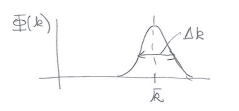
\includegraphics[width=0.5\linewidth]{resources/images/k_uncertainty.png}
    \caption{A graph of $\Phi(k)$ localized around $k=k_0$, with some uncertainty $\Delta k$.}
    \label{k_uncertainty}
\end{figure}

From Section \ref{stationary_phase_approximation}, we know that $|\Psi(x,\,0)|$ peaks when the phase is stationary at $k=k_0$, which occurs at $x=0$. Again, there must be some uncertainty $\Delta x$, as shown in Figure \ref{x_uncertainty}.

\begin{figure}[H]
    \centering
    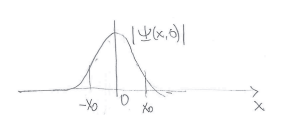
\includegraphics[width=0.5\linewidth]{resources/images/x_uncertainty.png}
    \caption{A graph of $|\Psi(x,0)|$ centered around $x=0$, with some uncertainty $\Delta x=x_0$.}
    \label{x_uncertainty}
\end{figure}

We write $k=k_0+\tilde{k}$. Then we have $$\Psi(x,\,0)=e^{ik_0x}\int\Phi(k_0+\tilde{k})e^{i\tilde{k}x}\,d\tilde{k}.$$Note that the relevant range of integration for $\tilde{k}$ is $[-\frac{\Delta k}{2},\,\frac{\Delta k}{2}]$. For $x=0$, the phase will be stationary for all $\tilde{k}$ and we will get a significant result. On the other hand, for $x\neq 0$, the phase will range over $[-\frac{\Delta k}{2}x,\,\frac{\Delta k}{2}x]$. The total phase excursion is thus $\Delta k\cdot x$. We will get a contribution to the integral as long as this quantity is not too large --- that is, as long as $\Delta k\cdot x\lesssim 1$. Therefore, $\Psi(x,\,0)$ will be sizable in an interval $x\in(-x_0,\,x_0)$ for $\Delta k\cdot x_0\approx 1$. The uncertainty in $x$ is $\Delta x=2x_0$, and since we are approximating, we drop the factor of 2. We therefore have $$\Delta k\,\Delta x\approx1.$$Note that nowhere in this argument did we use quantum mechanics; instead, this is simply a statement about wave packets and Fourier transforms. The physics comes in here: since $p=\hbar k$, we have $\Delta p=\hbar\,\Delta k$. Thus, we have $$\Delta p\,\Delta x\approx \hbar.$$With precise definitions, there is an exact result: $\Delta x\,\Delta p\geq \frac{\hbar}{2}$. This requires more background with uncertainties, which we will cover later. 

\begin{framedexpl}[Square $\Phi(k)$]
    Let $\Phi(k)=\frac{1}{\sqrt{\Delta k}}$ for $-\frac{\Delta k}{2}\leq k\leq\frac{\Delta k}{2}$ and $0$ everywhere else. Then we have $\Phi(k)=-\Phi(k)^*$, so $\Psi(x,\,0)$ is real. In fact,   $$\Psi(x,\,0)=\frac{1}{\sqrt{2\pi}}\int_{-\frac{\Delta k}{2}}^{\frac{\Delta k}{2}}\frac{1}{\sqrt{\Delta k}}e^{ikx}\,dk.$$
    Evaluating, $$\Psi(x,\,0)=\frac{1}{\sqrt{2\pi\Delta k}}\frac{e^{ikx}}{ix}\bigg]^\frac{\Delta k}{2}_{-\frac{\Delta k}{2}}=\sqrt{\frac{\Delta k}{2\pi}}\frac{\sin(\frac{\Delta k\,x}{2})}{(\frac{\Delta k\,x}{2})}.$$We display $\Psi(x,\,0)$ in Figure \ref{square_phi}. We estimate $\Delta x\approx\frac{2\pi}{\Delta k}$, so $\Delta x\,\Delta k\approx 2\pi$.
\end{framedexpl}

\begin{figure}[H]
    \centering        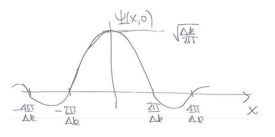
\includegraphics[width=0.5\linewidth]{resources/images/square_phi.png}
    \caption{A graph of $\Psi(x,0)$ for a square $\Phi(k)$.}
    \label{square_phi}
\end{figure}

\section{Time Evolution}
\subsection{Shape Changes in a Wave}\label{shape_changes}

Classical waves maintain a constant shape as they move. However, the Schrödinger equation is first-order in time, so quantum waves also spread outward. We have $$\Psi(x,\,t)=\frac{1}{\sqrt{2\pi}}\int\Phi(k)e^{ikx}e^{-i\omega(k)t}\,dk.$$As in Section \ref{group_velocity}, we expand $\omega(k)$ as $$\omega(k)= \omega(k_0)+ (k-k_0)\frac{d\omega(k)}{dt}\bigg|_{k_0}+\frac{1}{2}(k-k_0)^2\frac{d^2\omega}{dk^2}\bigg|_{k_0}+\ldots$$Recall that $\frac{d\omega}{dk}=\frac{dE}{dp}=\frac{d}{dp}\frac{p^2}{2m}=\frac{p}{m}=\frac{\hbar k}{m}$. Additionally, we have $\frac{d^2\omega}{dk^2}=\frac{\hbar}{m}$ and $\frac{d^3\omega}{dk^3}=0$. Thus, the series actually terminates after the quadratic term! $$\omega(k)= \omega(k_0)+ (k-k_0)\frac{d\omega(k)}{dt}\bigg|_{k_0}+\frac{1}{2}(k-k_0)^2\frac{d^2\omega}{dk^2}\bigg|_{k_0}$$Unlike in Section \ref{group_velocity}, we now consider the quadratic term, so $$e^{-i\omega(k)t}=e^{\ldots -i\frac{1}{2}(k-k_0)^2\frac{\hbar}{m}t}.$$Suppose we start with the wavepacket at $t=0$ and observe as it evolves in time. We have no significant shape change as long as $(k-k_0)^2\frac{\hbar}{m}t\ll 1$. We can estimate $(k-k_0)^2\approx(\Delta k)^2$, since the relevant $k$ terms are within the uncertainty of $\Phi(k)$. Thus, we have $(\Delta k)^2\frac{\hbar t}{m}\ll 1$, which can be rewritten as $$t\ll \frac{m\hbar}{(\Delta p)^2}.$$This is the range of $t$ for which the wave function will not undergo significant shape change. Additionally, we have from Section \ref{widths_uncertainties} that $\Delta x\, \Delta p\approx\hbar$, so we can also write $$t\ll\frac{m}{\hbar}(\Delta x)^2.$$Finally, we can rewrite this as $$\frac{\Delta p}{m}t\ll\Delta x.$$
The packet changes shape because the group velocity $\frac{d\omega}{dk}$ is not constant throughout the packet. The term $\frac{\Delta p}{m}$ represents this uncertainty in the group velocity. There will be appreciable shape change when the uncertainty in velocity, propagating through time, produces position uncertainty comparable to the width $\Delta x$ of the wavepacket. 

\begin{framedquest*}
    For an electron, we have $\Delta x\approx 10^{-10}m$. How long does it remain localized?
\end{framedquest*}

\begin{framedansw*}
    The electron remains localized for time $$t\approx\frac{m}{\hbar}(\Delta x)^2=\frac{mc^2}{\hbar c}\frac{(\Delta x)^2}{c}\approx 10^{-16}s.$$The miniscule time scales for which electrons remain localized provide a technological difficulty for particle accelerators.    
\end{framedansw*}

\subsection{Evolving the Free Particle Wavepacket}
\label{evolving_free_particle}

Suppose you know $\Psi(x,\,0)$ for a free particle and want to find $\Psi(x,\,t)$. This is accomplished in a few steps.

\begin{enumerate}
    \item Calculate $\Phi(k)$ using the Fourier inversion theorem: $\Phi(k)=\frac{1}{\sqrt{2\pi}}\int\Psi(x,\,0)e^{-ikx}\,dx$.
    \item With this, write $\Psi(x,\,0)=\frac{1}{\sqrt{2\pi}}\int \Phi(k)e^{ikx}\,dk$.
    \item To evolve this wavefunction, simply write $$\Psi(x,\,t)=\frac{1}{\sqrt{2\pi}}\int\Phi(k)e^{i(kx-\omega(k)t)}\,dk.$$We have as always that $\hbar\omega(k)=\frac{\hbar^2 k^2}{2m}$. This is a solution to the Schrödinger Equation since it expresses $\Psi(x,\,t)$ as a linear combination of plane waves, each of which is a solution. Since it reduces to $\Psi(x,\,0)$ at $t=0$, it is the unique solution to the Schrödinger Equation that matches the initial conditions.
    \item Perform the integral over $k$, if possible.
\end{enumerate}

\begin{framedexpl}[Evolving the Gaussian]
    Consider the Gaussian wavefunction $$\Psi_a(x,\,0)=\frac{e^{-\frac{x^2}{4a^2}}}{(2\pi)^{1/4}\sqrt{a}}.$$ Since the relevant length scale here is $a$, from Section \ref{shape_changes}, we estimate that the relevant time scale is $\tau\approx\frac{m}{\hbar}a^2$. In fact, it turns out that $\tau=\frac{2ma^2}{\hbar}$. The answer is a bit messy, but we end up with $$|\Psi_a(x,\,t)|^2=\frac{1}{\sqrt{2\pi}}\frac{1}{a(t)}e^{-x^2/2a^2(t)}.$$ Here, $a(t)$ is a time-dependent width given by $a(t)=a\sqrt{1+t^2/\tau^2}$.
\end{framedexpl}

\section{Momentum Space}
\subsection{Delta Functions}\label{delta_functions}

So far, we've been working with wavefunctions that give you the probability of finding a particle at a given position. This is called the \textbf{position space} or \textbf{coordinate space} representation of quantum mechanics. However, we've seen that position and momentum are closely related, and we can reformulate quantum mechanics in terms of \textbf{momentum space}.

Recall from Theorem \ref{fourier_inversion} that $\Psi(x)$ is related to its Fourier transform $\Phi(x)$ by the equations \begin{align*}\Psi(x)&=\frac{1}{\sqrt{2\pi}}\int\Phi(k)e^{ikx}\,dk,\\\Phi(k)&=\frac{1}{\sqrt{2\pi}}\int\Psi(x)e^{-ikx}\,dx.\end{align*}We can think of $\Phi(k)$ as containing the same information as $\Psi(x)$, in that given either one, we can find the other.

Now we have an expression for $\Psi(x)$ in terms of $\Phi(k)$, and vice versa. What if we substitute the expression for $\Phi(k)$ into the first equation? We get \begin{align*}\Psi(x)&=\frac{1}{\sqrt{2\pi}}\int dk\,e^{ikx}\frac{1}{\sqrt{2\pi}}\int\Psi(x')e^{-ikx'}\,dx'\\&=\int dx'\,\Psi(x')\,\underbrace{\frac{1}{2\pi}\int dk\,e^{ik(x-x')}}.\end{align*}Consider the factor indicated by the brace. If $x=x'$, it goes to infinity. However, if $x\neq x'$, it oscillates and prevents the integral from having any contribution. Thus, the factor effectively reduces the $x'$ integral to an evaluation at $x$.\footnote{This is a very hand-wavey argument that probably seems very sketchy --- much of the problem is that the delta function is not really a \textit{function} at all, but a \textit{distribution}, or \textit{generalized function}. All that we need to know about it is that it reduces integrals of other functions to evaluations at points. That being said, if you really need a more rigorous explanation of why this is true, you can check out \href{https://math.stackexchange.com/questions/2340094/why-frac12-pi-int-infty-inftyeiwt-xdw-is-the-dirac-delta-func?noredirect=1&lq=1}{this} Math StackExchange post.} We call it the \textbf{delta function} $$\delta(x-x')=\frac{1}{\sqrt{2\pi}}\int_{-\infty}^{\infty}dk\,e^{ik(x-x')}.$$Note that $\delta(0)=\infty$, and $\delta(ax)=\frac{1}{|a|}\delta(x)$.

\subsection{Parseval's Theorem}\label{section-parseval}

We have found a deep relationship between $\Psi(x)$ and its Fourier transform $\Phi(k)$. We now wish to know how the normalization condition for $\Psi(x)$ (from Section \ref{normalization}) looks in terms of $\Phi(k)$. We have $$\int dx\,\Psi^*(x)\Psi(x)=\int dx\,\frac{1}{\sqrt{2\pi}}\int dk\,\Phi^*(k)e^{-ikx}\,\frac{1}{\sqrt{2\pi}}\int dk'\,\Phi(k')e^{ikx}.$$We have no chance of computing the $k$ and $k'$ integrals, since $\Phi$ is an abstract function. Thus, we rewrite this expression to perform the $x$ integral first: \begin{align*}\int dx\,\Psi^*(x)\Psi(x)&=\int dk\,\Phi^*(k)\int dk'\,\Phi(k')\,\frac{1}{2\pi}\int dx\,e^{i(k'-k)x}\\&=\int dk\,\Phi^*(k)\int dk'\,\Phi(k')\;\delta(k'-k)\\&=\int dk\,\Phi^*(k)\Phi(k).\end{align*}Note that we used the fact that the delta function factor $\delta(k'-k)$ has the effect of evaluating the inner integral at $k$. Our final result is therefore $\int dx\,|\Psi(x)|^2=\int dk\,|\Phi(k)|^2$. This is called \textbf{Parseval's Theorem}:\footnote{In mathematics, a more general version is called Plancherel's theorem.}

\begin{framedthm}[Parseval's Theorem]\label{parseval}
   For a wavefunction $\Psi(x)$ and its Fourier transform $\Phi(k)$, we have $$\int dx\,|\Psi(x)|^2=\int dk\,|\Phi(k)|^2.$$ 
\end{framedthm}

Since we physically associate wavefunctions with momentum eigenstates, we rewrite Parseval's Theorem in terms of $p=\hbar k$. We define $\tilde{\Phi}(p)=\Phi(k)$. We then have \begin{align*}\Psi(x)&=\frac{1}{\sqrt{2\pi}}\int \tilde{\Phi}(p)e^{ipx/\hbar}\frac{dp}{\hbar}\\ \tilde{\Phi}(p)&=\frac{1}{\sqrt{2\pi}}\int\Psi(x)e^{-ipx/\hbar}\,dx\end{align*}For symmetry, we define $\Phi(p)$ so that $\tilde{\Phi}(p)=\Phi(p)\sqrt{\hbar}$. Then these equations become \begin{align*}\Psi(x)&=\frac{1}{\sqrt{2\pi\hbar}}\int {\Phi}(p)e^{ipx/\hbar}dp\\ {\Phi}(p)&=\frac{1}{\sqrt{2\pi\hbar}}\int\Psi(x)e^{-ipx/\hbar}\,dx\end{align*}After a lot of algebra and canceling variables, Theorem \ref{parseval} is unchanged: $$\int dx\,|\Psi(x)|^2=\int dp\,|\Phi(p)|^2.$$

Just as we interpreted $|\Psi(x)|^2\,dx$ in Section \ref{born_rule}, we interpret $|\Phi(p)|^2\,dp$ as the probability to find the particle with momentum in the range $[p,\,p+dp]$. 

\subsection{Fourier Transforms in Three Dimensions}\label{3d-fourier}


In three dimensions, the equations from Theorem \ref{fourier_inversion} take the form \begin{align*}\mathbf{\Psi}(\mathbf{x})&=\frac{1}{(2\pi\hbar)^{3/2}}\int d^3\mathbf{p}\,\mathbf{\Phi}(\mathbf{p})e^{i\mathbf{p}\cdot\mathbf{x}/\hbar},\\ \mathbf{\Phi}(\mathbf{p})&=\frac{1}{(2\pi\hbar)^{3/2}}\int d^3\mathbf{x}\,\mathbf{\Psi}(\mathbf{x})e^{-i\mathbf{p}\cdot\mathbf{x}/\hbar}.\end{align*}Furthermore, there is a delta function in three dimensions, given by $$\delta^3(\mathbf{x}-\mathbf{x}')=\frac{1}{(2\pi)^3}\int d^3\mathbf{k}\,e^{i\mathbf{k}\cdot(\mathbf{x}-\mathbf{x'})}.$$Then we can derive Theorem \ref{parseval} in three dimensions just as in one dimension: $$\int d^3\mathbf{x}\,|\mathbf{\Psi}(\mathbf{x})|^2=\int d^3\mathbf{p}\,|\mathbf{\Phi}(\mathbf{p})|^2.$$

    \chapter{Expectation Values \& Eigenstates}
    \section{Expectation Values}

\subsection{Expectation Value of Position}\label{expected_position}

Consider a random variable $Q$ that can take values in the set $\{Q_1,\ldots,Q_n\}$ with probabilities $\{P_1,\ldots,P_n\}$. Then we define the \textbf{expectation value}, or expected value, of $Q$ to be the average value we would expect after measuring $Q$ many times: $$\langle Q\rangle=\sum_{i=1}^nQ_ip_i.$$In a quantum system, the probability that a particle is found in the range$[x,\,x+dx]$ is given by $\Psi^*(x,\,t)\Psi(x,\,t)\,dx$. Thus, the expectation value of $x$, denoted by $\langle\hat{x}\rangle$, is $$\langle\hat{x}\rangle=\int x\,\Psi^*(x,\,t)\Psi(x,\,t)\,dx.$$Note that this quantity may depend on time.

\begin{framedrmk*}[Physical interpretation of the expectation value]
    If we were to create many copies of a physical system and measure the position of the particle in each one, the average would converge to $\langle\hat{x}\rangle$.
\end{framedrmk*}

\subsection{Expectation Value of Momentum}\label{expected_momentum}

Recall that $|\Phi(p)|^2\,dp$ is the probability of finding the particle with momentum in the range $[p,\,p+dp]$. Then the expectation value of momentum is given by $$\langle\hat{p}\rangle=\int p\,|\Phi(p)|^2\,dp.$$It would be helpful to write this formula in position space (in terms of $x$). We expand \begin{align*}\langle\hat{p}\rangle&=\int p\,\Phi^*(p)\Phi(p)\,dp\\&=\int p\,dp\int\frac{dx'}{\sqrt{2\pi\hbar}}e^{ipx'/\hbar}\Psi^*(x')\int\frac{dx}{\sqrt{2\pi\hbar}}e^{ipx/\hbar}\Psi(x)\\&=\frac{1}{2\pi\hbar}\int dx'\,\Psi^*(x')\int dx\,\Psi(x)\int dp\,p\,e^{ipx'/\hbar}e^{-ipx/\hbar}.\end{align*}Note that $$p\,e^{ipx'/\hbar}e^{-ipx/\hbar}=\bigg(-\frac{\hbar}{i}\frac{\partial}{\partial x}\bigg)e^{ipx'/\hbar}e^{-ipx/\hbar},$$since the partial derivative applies only to the second exponential factor. Thus we can substitute \begin{align*}\langle\hat{p}\rangle&=\frac{1}{2\pi\hbar}\int dx\,\Psi^*(x')\int dx\,\Psi(x)\int dp\,\bigg(-\frac{\hbar}{i}\frac{\partial}{\partial x}\bigg)\,e^{ipx'/\hbar}e^{-ipx/\hbar}\\&=\int dx'\Psi^*(x')\int dx\,\Psi(x)\bigg(-\frac{\hbar}{i}\frac{\partial}{\partial x}\bigg)\frac{1}{2\pi\hbar}\int dp\,e^{ip(x'-x)/\hbar}.\end{align*}Letting $p=\hbar u$ in the final integral, we have $$\frac{1}{2\pi\hbar}\int dp\,e^{ip(x'-x)/\hbar}=\frac{1}{2\pi}\int du\,e^{iu(x-x')}=\delta(x-x').$$Now consider the integral $$\int dx\,\Psi(x)\bigg(-\frac{\hbar}{i}\frac{\partial}{\partial x}\bigg)\delta(x-x').$$This is of the form $\int u\,dv$, where $u=\Psi$ and $v=-\frac{\hbar}{i}\delta(x-x')$. By integration by parts, we have $\int u\,dv=uv-\int v\,du$. Since $\Psi$ vanishes at infinity (which was one of our requirements from Section \ref{normalization}), the $uv$ term disappears. Thus, we have $$\int dx\,\Psi(x)\bigg(-\frac{\hbar}{i}\frac{\partial}{\partial x}\bigg)\delta(x-x')=\int dx\,\bigg(\frac{\hbar}{i}\frac{\partial\Psi}{\partial x}\bigg)\delta(x-x').$$Substituting this into our equation for $\langle\hat{p}\rangle$, we have \begin{align*}\langle\hat{p}\rangle&=\int dx'\Psi^*(x')\int dx\,\bigg(\frac{\hbar}{i}\frac{\partial\Psi}{\partial x}\bigg)\delta(x-x')\\&=\int dx\,\frac{\hbar}{i}\frac{\partial\Psi}{\partial x}\int dx'\Psi^*(x')\delta(x-x').\end{align*}The delta function $\delta(x-x')$ evaluates $\Psi^*(x')$ at $x$, so we finally have that $$\langle\hat{p}\rangle=\int p\,|\Phi(p)|^2\,dp=\int dx\,\frac{\hbar}{i}\frac{\partial\Psi}{\partial x}\Psi^*=\int dx\,\Psi^*(x)\frac{\hbar}{i}\frac{\partial}{\partial x}\Psi(x).$$Including the time dependence, we have $$\langle\hat{p}\rangle=\int dx\,\Psi^*(x,t)\,\hat{p}\,\Psi(x,t).$$In general, for an operator $\hat{Q}$, we have that the expectation value of $\hat{Q}$ is given by $$\boxed{\langle\hat{Q}\rangle=\int dx\,\Psi^*(x,t)\,\hat{Q}\,\Psi(x,t)}$$

\begin{framedexpl}[Expectation value of the kinetic energy operator]
    Consider the kinetic energy operator $\hat{T}=\frac{\hat{p}^2}{2m}=-\frac{\hbar^2}{2m}\frac{\partial^2}{\partial x^2}$. Then we have $$\langle\hat{T}\rangle= \int dx\,\Psi^*\bigg(-\frac{\hbar^2}{2m}\frac{\partial^2}{\partial x^2}\Psi\bigg).$$Alternatively, in momentum space, we have $$\langle\hat{T}\rangle=\int dp\,\frac{p^2}{2m}|\Phi(p)|^2=\int dp\,\Phi^*(p)\frac{p^2}{2m}\Phi(p).$$
\end{framedexpl}

\subsection{Time Dependence of Expectation Values}\label{time_dependence_expectation}

Consider the time derivative of the expectation value of an operator $\hat{Q}$. We have $$\frac{d}{dt}\langle\hat{Q}\rangle=\frac{d}{dt}\int dx\,\Psi^*\hat{Q}\Psi=\int dx\,\bigg(\frac{\partial\Psi^*}{\partial t}\hat{Q}\Psi+\Psi^*\hat{Q}\frac{\partial\Psi}{\partial t}\bigg).$$From the Schrödinger equation, we have $$\frac{d}{dt}\langle\hat{Q}\rangle=\int dx\,\bigg(\frac{i}{\hbar}(\hat{H}\Psi)^*\hat{Q}\Psi-\frac{i}{\hbar}\Psi^*\hat{Q}\hat{H}\Psi\bigg).$$Multiplying both sides by $i\hbar$, we have \begin{align*}i\hbar\frac{d}{dt}\langle\hat{Q}\rangle&=\int dx\,(\Psi^*\hat{Q}\hat{H}\Psi-(\hat{H}\Psi)^*\hat{Q}\Psi)\\&=\int dx\,(\Psi^*\hat{Q}\hat{H}\Psi-\Psi^*\hat{H}\hat{Q}\Psi)\\&=\int dx\,\Psi^*(\hat{Q}\hat{H}-\hat{H}\hat{Q})\Psi\\&=\int dx\,\Psi^*[\hat{Q},\hat{H}]\Psi.\end{align*}Therefore, we have the fundamental relationship $$i\hbar\frac{d}{dt}\langle\hat{Q}\rangle=\langle[\hat{Q},\hat{H}]\rangle.$$For example, for a free particle, $\hat{p}$ commutes with $\hat{H}=\frac{\hat{p}^2}{2m}$, so the expectation value of the momentum does not change with time.

\subsection{Expectation Values of Hermitian Operators}\label{expected_hermitian}

In Definition \ref{hermitian}, we defined an operator $\hat{Q}$ to be Hermitian if, for any $\Psi_1$ and $\Psi_2$, we had $$\int dx\,\Psi_1^*\hat{Q}\Psi_2 = \int dx\,(\hat{Q}\Psi_1)^*\Psi_2.$$We now introduce a shorthand for the integrals of pairs of functions: $$(\Psi_1,\Psi_2)=\int \Psi_1^*\Psi_2\,dx.$$This is called the \textbf{inner product} of $\Psi_1$ and $\Psi_2$, and it is a generalization of the vector dot product that obeys the properties $(a\Psi_1,\Psi_2)=a^*(\Psi_1,\Psi_2)$ and $(\Psi_1,a\Psi_2)=a(\Psi_1,\Psi_2)$.\footnote{This is a simplified version of \href{https:\/\/en.wikipedia.org\/wiki\/Bra\%E2\%80\%93ket\_notation}{Dirac notation}, 
which represents wavefunctions as vectors and operators as matrices.} The condition of Hermiticity can be more briefly stated as$$(\Psi_1,\hat{Q}\Psi_2)=(\hat{Q}\Psi_1,\Psi_2).$$We can also express the expectation value of $\hat{Q}$ in a normalized wavefunction $\Psi$, which we found to be $$\langle\hat{Q}\rangle_\psi=(\Psi,\hat{Q}\Psi).$$We proceed by stating and proving some claims about a general Hermitian operator acting on a normalized wavefunction $\Psi$.

\begin{framedprop}[$\langle\hat{Q}\rangle_\Psi$ is real]\label{9.1.1}

\begin{proof}
    We show that $(\langle\hat{Q}\rangle_\Psi)^*=\langle\hat{Q}\rangle_\Psi$. We have $$(\langle\hat{Q}\rangle_\Psi)^*=\int dx\,(\Psi^*\hat{Q}\Psi)^*=\int dx\,\Psi(\hat{Q}\Psi)^*=\int dx\,(\hat{Q}\Psi)^*\Psi.$$ Since $\hat{Q}$ is Hermitian, $$\int dx\,(\hat{Q}\Psi)^*\Psi=\int dx\,\Psi^*\hat{Q}\Psi=\langle\hat{Q}\rangle_\Psi.$$Thus, $\langle\hat{Q}\rangle_\Psi$ is real.
\end{proof}
\end{framedprop}

Note that $\hat{Q}\Psi$ is a \textit{wavefunction} that we can take the complex conjugate of; we never think about the complex conjugate of the \textit{operator} $\hat{Q}$.

\section{Eigenvalues \& Eigenfunctions}

\subsection{Eigenvalues of Hermitian Operators}\label{eigenvalues}

We define eigenvectors and eigenvalues of operators analogously to their definitions for matrices: $\Psi$ is an eigenvector of $\hat{Q}$ with associated eigenvalue $q$ if $\hat{Q}\Psi=q\Psi$. We can also call $\Psi$ an \textbf{eigenstate} or \textbf{eigenfunction} of $\hat{Q}$.

\begin{framedprop}[The eigenvalues of $\hat{Q}$ are real]\label{9.1.2}
    \begin{proof}Suppose $\Psi_1$ is an eigenstate of $\hat{Q}$ with eigenvalue $q_1$. Then the expectation value of $\hat{Q}$ in $\Psi_1$ is $$\langle\hat{Q}\rangle_{\Psi_1}=\int dx\,\Psi_1^*\hat{Q}\Psi_1=\int dx\,\Psi_1^*q_1\Psi_1=q_1\int dx\,\Psi_1^*\Psi_1.$$However, in Proposition \ref{9.1.1}, we showed that $\langle\hat{Q}\rangle_{\Psi_1}$ is real. Since $\int dx\,\Psi_1^*\Psi_1$ must be real, $q_1$ must also be real. Note that if the eigenfunction $\Psi_1$ is normalized, the expectation value of $\hat{Q}$ in $\Psi_1$ is exactly the eigenvalue $q_1$.\end{proof}
\end{framedprop}

\subsection{Eigenfunctions of Hermitian Operators}\label{eigenfunctions}

Consider the collection of eigenfunctions and eigenvalues of the Hermitian operator $\hat{Q}$: \begin{align*}\hat{Q}\Psi_1&=q_1\Psi_1,\\\hat{Q}\Psi_2&=q_2\Psi_2,\\\vdots\quad&\qquad\,\vdots\end{align*}This list may be finite or infinite.

\begin{framedprop}[The eigenfunctions of $\hat{Q}$ can be organized to satisfy orthonormality: $(\Psi_i,\Psi_j)=\delta_{ij}$]\label{9.2.1}

    \begin{proof}For $i=j$, this simply claims that we can normalize all the eigenfunctions, which we can certainly do. We also require that different eigenfunctions are orthogonal. We prove this for the case of $q_i\neq q_j$.

    We evaluate $(\Psi_i,\hat{Q}\Psi_j)$ in two different ways. First, $(\Psi_i,\hat{Q}\Psi_j)=(\Psi_1,q_j\Psi_j)=q_j(\Psi_i,\Psi_j)$. However, by Hermiticity and Proposition \ref{9.1.2}, we also have $(\Psi_i,\hat{Q}\Psi_j)=(\hat{Q}\Psi_i,\Psi_j)=(q_i\Psi_i,\Psi_j)=q_i(\Psi_i,\Psi_j)$. Thus, we have $$(q_i-q_j)(\Psi_i,\Psi_j)=0.$$Since $q_i\neq q_j$, this can only be true if $(\Psi_i,\Psi_j)=0$.

    This proof does not hold if there are \textbf{degeneracies} in the spectrum of $\hat{Q}$ -- that is, if there are multiple eigenfunctions with the same eigenvalue. In this case, we would have to show that it is possible to choose $\text{linear combinations}$ of the degenerate eigenfunctions that are mutually orthogonal. This can be done via the Gram-Schmidt process from linear algebra.\footnote{This is covered in Lakeside's linear algebra course. If you're curious, ask a math teacher!} \end{proof}
\end{framedprop}

That brings us to our most important result, which we will not prove,\footnote{Again, ask a linear algebra teacher!} but which is quite literally a necessary condition for all the rest of the physics we will do in this course. It is called the \textbf{spectral theorem}, and has analogs in all sorts of math fields, including calculus and graph theory!

\begin{framedthm}[Spectral Theorem]\label{spectral}
    The eigenfunctions of $\hat{Q}$ form an \textbf{orthonormal basis} of the possible wavefunctions: any reasonable $\Psi$ can be expressed as a combination of eigenfunctions. In other words, given an arbitrary wavefunction $\Psi$ and the eigenfunctions $\Psi_i$ of $\hat{Q}$, we can write $$\Psi=\sum_i\alpha_i\Psi_i$$for calculable coefficients $\alpha_i$. Indeed, given the eigenfunctions, we have that $\alpha_i=(\Psi_i,\Psi)$, which can be proven by doing the integral: $$\int dx\,\Psi^*_i\sum_j\alpha_p\Psi_j=\sum_j\alpha_j\int dx\,\Psi_i^*\Psi_j=\sum_j\delta_{ij}=\alpha_i.$$Additionally, we have \begin{align*}
    \int|\Psi|^2dx &= \int(\sum_i\alpha_i\Psi_i)^*\sum_j\alpha_j\Psi_j dx \\ &= \sum_i\sum_j\alpha_i^*\alpha_j\int dx\,\Psi_i^*\Psi_j\\ &=\sum_i\sum_j\alpha^*_i\alpha_j\delta_{ij}\\ &=\sum_i\alpha_i^*\alpha=\sum_i|\alpha_i|^2.
    \end{align*}

    If $\Psi$ is normalized, we have $$\sum_i|\alpha_i|^2=1.$$
\end{framedthm}

We are now finally able to state the measurement postulate, which is how we understand that Hermitian operators represent observables. It is an \textit{axiom}, which means it cannot be proven. Instead, it is a fact that we take to be true because it aligns with all our experiments.

\begin{framedthm}[Measurement postulate]\label{measurement}
   If we measure the Hermitian operator $\hat{Q}$ with eigenfunctions $\Psi_i$ in the state $\Psi=\sum_i\alpha_i\Psi_i$, the possible outcomes for the measurement are the eigenvalues $q_1,q_2,\ldots$. The probability $p_i$ to measure $q_i$ is given by $$p_i=|\alpha_i|^2.$$After the measurement (yielding $q_i$), the state of the system becomes $$\Psi'=\Psi_i.$$This is called the \textbf{collapse} of the wavefunction. 
\end{framedthm} 

Wavefunction collapse implies that repeated measurements will always yield the same result with no uncertainty. A small subtlety occurs with degenerate eigenstates. If $\Psi=(\alpha_i\Psi_i+\alpha_k\Psi_k)+\ldots$, where $\Psi_i$ and $\Psi_k$ have the same eigenvalue $q$, then measuring $q$ causes the wavefunction to collapse to the \textit{sum} of $\Psi_i$ and $\Psi_k$:$$\Psi'=\frac{\alpha_i\Psi_i+\alpha_k\Psi_k}{\sqrt{|\alpha_i|^2+|\alpha_j|^2}}.$$

\begin{framedrmk*}[Copenhagen interpretation]
    Theorem \ref{measurement} is an axiom of the \textit{Copenhagen interpretation} of quantum mechanics, which was developed by Werner Heisenberg, Max Born, and Niels Bohr. The Copenhagen interpretation treats quantum mechanics as intrinsically nondeterministic, with probabilistic measurements as given by the measurement postulate. What makes quantum mechanics nondeterministic is that when you make a measurement, you know you will get an eigenvalue, but you do not know which one.

    Other interpretations of quantum mechanics exist. For example, the many worlds hypothesis includes the observer in the system to resolve the phenomenon of wavefunction collapse.
\end{framedrmk*}

Note that Theorem \ref{spectral} is necessary to make measurements of a general physical system, since we need to be able to express any $\Psi$ in terms of the eigenfunctions of any Hermitian operator.

\subsection{Consistency Condition}\label{consistency}

Suppose we have an expansion $\Psi=\sum_i\alpha_i\Psi_i$ of a wavefunction in terms of the eigenfunctions of some Hermitian operator $\hat{Q}$. We wish to find the expectation value of $\hat{Q}$: \begin{align*}\langle\hat{Q}\rangle&=\int dx\,\sum_i\alpha_i^*\Psi_i^*\hat{Q}\sum_j\alpha_j\Psi_j\\&=\sum_{i,j}\alpha_i^*\alpha_j\int dx\,\Psi_i^*\hat{Q}\Psi_j\\&=\sum_{i,j}\alpha_i^*\alpha_jq_j\int dx\,\Psi_i^*\Psi_j\\&=\sum_{i,j}\alpha_i^*\alpha_jq_i\delta_{ij}\\&=\sum_i|\alpha_i|^2q_i=\sum_ip_iq_i.\end{align*}This is exactly what it should be: the $q_i$ are the possible measurements by Theorem \ref{measurement}, and the expected value is their weighted sum by the probabilities $p_i=|\alpha_i|^2$.

\subsection{Extended Example: Particle on a Circle}\label{particle-on-a-circle}

Consider a free particle on a circle $x\in [0,L)$, where we set the point $x=L$ equivalent to $x=0$. A wavefunction $\Psi(x)$ on the circle must satisfy the periodicity condition $\Psi(x+L)=\Psi(x)$. Suppose that at some fixed time we have $$\Psi(x)=\sqrt{\frac{2}{L}}(\frac{1}{\sqrt{3}}\sin\frac{2\pi x}{L}+\sqrt{\frac{2}{3}}\cos\frac{6\pi x}{L}).$$It is easy to verify that this wavefunction satisfies the periodicity condition.

\begin{framedquest*}
    If you measure momentum in this state, what are the possible results and their probabilities?
\end{framedquest*}

\begin{framedansw*}
    We must find the set of momentum eigenstates and rewrite $\Psi$ as a superposition of these states. Momentum eigenstates are of the form $e^{ikx}$. By the periodicity condition, we must have $k=\frac{2\pi m}{L}$ for $m\in\mathbb{Z}$. Thus we write the momentum eigenstates $\Psi_m(x)=Ne^{\frac{2\pi imx}{L}}$ for some normalization constant $N$. Indeed, normalizing gives $N=\frac{1}{\sqrt{L}}$.

    We now apply the momentum operator to a momentum eigenstate $\Psi_m$: $$\hat{p}\Psi_m(x)=\frac{\hbar}{i}\frac{\partial}{\partial x}\frac{1}{\sqrt{L}}e^{\frac{2\pi imx}{L}}=\frac{\hbar 2\pi m}{L}\Psi_m.$$Thus, the eigenvalue of the eigenstate $\Psi_m$ is $$p_m=\frac{\hbar 2\pi m}{L}.$$Now we have to rewrite $\Psi$ as a superposition of these eigenstates: $$\Psi(x)=\sqrt{\frac{2}{3}}\frac{1}{2i}\frac{1}{\sqrt{L}}(e^{\frac{2\pi ix}{L}}-e^{-\frac{2\pi ix}{L}})+\frac{2}{\sqrt{3}}\frac{1}{2}\frac{1}{\sqrt{L}}(e^{\frac{6\pi ix}{L}}+e^{-\frac{6\pi ix}{L}}).$$Therefore, we have $$\Psi(x)=\sqrt{\frac{2}{3}}\frac{1}{2i}\Psi_1(x)-\sqrt{\frac{2}{3}}\frac{1}{2i}\Psi_{-1}(x)+\frac{1}{\sqrt{3}}\Psi_3(x)+\frac{1}{\sqrt{3}}\Psi_{-3}(x).$$This is the key result; we can now read off the possible values of $p$ and their probabilities.

    \centering
    \begin{tabular}{|c|c|}
        \hline
        Momentum & Probability \\
        \hline
        $p=\frac{2\pi\hbar}{L}$ & $P=|\sqrt{\frac{2}{3}}\frac{1}{2i}|^2=\frac{1}{6}$ \\
        $p=-\frac{2\pi\hbar}{L}$ & $P=|-\sqrt{\frac{2}{3}}\frac{1}{2i}|^2=\frac{1}{6}$ \\
        $p=\frac{6\pi\hbar}{L}$ &
        $P=|\sqrt{\frac{1}{3}}|^2=\frac{1}{3}$ \\
        $p=-\frac{6\pi\hbar}{L}$ &
        $P=|\sqrt{\frac{1}{3}}|^2=\frac{1}{3}$\\
        \hline
    \end{tabular}

\end{framedansw*}

\subsection{Defining Uncertainty}

For a random variable $Q$ with possible values $Q_1,\ldots,Q_n$ and corresponding probabilities $p_1,\ldots,p_n$, the expected value of $Q$ is $\bar{Q}=\sum_i p_iQ_i$. The uncertainty in $Q$ is represented by the \textbf{standard deviation} of $Q$: $$(\Delta Q)^2 = \sum_ip_i(Q_i-\bar{Q})^2.$$Notice that if $\Delta Q=0$, we have $Q_i=\bar{Q}$ for all $i$; that is, $Q$ is constant. We can expand the right-hand side to get \begin{align*}(\Delta Q)^2&=\sum_ip_iQ_i^2-2\sum_ip_iQ_i\bar{Q}+\sum_ip_i\bar{Q}^2\\&=\overline{Q^2}-2\bar{Q}\bar{Q}+(\bar{Q})^2\\&=\overline{Q^2}-\bar{Q}^2.\end{align*}Since by definition $(\Delta Q)^2\geq 0$, we have the interesting inequality $$\overline{Q^2}\geq \bar{Q}^2.$$Now let us consider the quantum mechanical case. Let $\hat{Q}$ be a Hermitian operator. We define the uncertainty of $\hat{Q}$ in a state $\Psi$ by the relation $$(\Delta\hat{Q})^2_\Psi=\langle\hat{Q}^2\rangle_\Psi-\langle\hat{Q}\rangle^2_\Psi.$$For brevity, we will omit the $\Psi$ subscript.

\begin{framedprop}
    \label{9.5.1}
    The uncertainty can also be written as the expectation value of the square of the difference between the operator and its expectation value: $$(\Delta Q)^2=\langle(\hat{Q}-\langle\hat{Q}\rangle)^2\rangle$$Note that this implies that $\Delta Q$ is nonnegative.

    \begin{proof}
    We evaluate $$\langle(\hat{Q}-\langle\hat{Q}\rangle)^2\rangle=\langle\hat{Q}^2-2\hat{Q}\langle\hat{Q}\rangle+\langle\hat{Q}\rangle^2\rangle.$$By linearity, this equals $$\langle\hat{Q}^2\rangle-2\langle\hat{Q}\rangle\langle\hat{Q}\rangle+\langle\hat{Q}\rangle^2=\langle\hat{Q}^2\rangle-\langle\hat{Q}\rangle^2.$$By the definition of uncertainty, we have the desired equation.
\end{proof}
\end{framedprop}

\begin{framedprop}\label{9.5.2}
    The uncertainty can be written as the integral of the square of the norm of $(\hat{Q}-\langle\hat{Q}\rangle)\Psi$:$$(\Delta Q)^2=\int_{-\infty}^{\infty}dx\,\bigg|(\hat{Q}-\langle\hat{Q}\rangle)\Psi(x)\bigg|^2.$$

    \begin{proof} We start with $$\langle(\hat{Q}-\langle\hat{Q}\rangle)^2\rangle=\int dx\,\Psi^*(\hat{Q}-\langle\hat{Q}\rangle)(\hat{Q}-\langle\hat{Q}\rangle)\Psi.$$Since $\hat{Q}$ is Hermitian and $\langle\hat{Q}\rangle$ is a real number, the operator $(\hat{Q}-\langle\hat{Q}\rangle)$ is Hermitian. Thus, we can express this as $$\int dx\,\bigg((\hat{Q}-\langle\hat{Q}\rangle)\Psi\bigg)^*\bigg((\hat{Q}-\langle\hat{Q}\rangle)\Psi\bigg)=\int dx\,\bigg|(\hat{Q}-\langle\hat{Q}\rangle)\Psi(x)\bigg|^2.$$From Proposition \ref{9.5.1}, this equals $(\Delta Q)^2$. \end{proof}
\end{framedprop}

We now consider what it means for $\Delta Q$ to be $0$. If $\Psi$ is a (normalized) eigenstate of $\hat{Q}$ with eigenvalue $\lambda$, we have $\hat{Q}\Psi=\lambda\Psi$. Multiplying both sides by $\Psi^*$ and integrating, we have $$\langle\hat{Q}\rangle=\int dx\,\Psi^*\hat{Q}\Psi=\lambda\int dx\,\Psi^*\Psi=\lambda.$$Therefore, the eigenvalue of $\Psi$ is simply the expectation value of $\hat{Q}$ in $\Psi$. We then have $$\langle(\hat{Q}-\langle\hat{Q}\rangle)^2\rangle=(\Delta Q)^2=0$$by Proposition \ref{9.5.1}. On the other hand, if $\Delta Q = 0$, by Proposition \ref{9.5.2}, we must have $\langle(\hat{Q}-\langle\hat{Q}\rangle)\rangle=0$, which implies that $\hat{Q}\Psi=\langle\hat{Q}\rangle\Psi$. We see that the uncertainty of $\hat{Q}$ in state $\Psi$ is $0$ if and only if $\Psi$ is an eigenstate of $\hat{Q}$.

\begin{framedrmk*}[Uncertainty in symmetric wavefunctions]
    If $\Psi$ is symmetric about the origin, the expectation value of $x$ is $0$, so we have $$(\Delta x)^2=\langle x^2\rangle.$$
\end{framedrmk*}


    \chapter{Solving the Schrödinger Equation in One Dimension}
    \section{Stationary States}

\subsection{Introduction to Stationary States}\label{stationary_states}

We have now, after 51 pages, finally accumulated the necessary knowledge to begin solving quantum systems. But first, we must define what we are even trying to solve for.

In classical mechanics, we often wish to know the position $x(t)$ of a particle at a time $t$. The particle may be interacting with other particles or fields; we can represent these interactions by giving the particle some potential energy $V(x)$. 

In quantum mechanics, particles have indeterminate positions, so we cannot simply solve for some position function $x(t)$. Instead, we search for the \textit{state} of the particle, $\Psi(x,t)$. Often, in order to find the possible wavefunctions, we will also need to solve for the allowed energy values of quantum systems. 

For reasons that will soon become clear, we only care about \textbf{stationary states} of quantum systems. A stationary state has factorizable space and time dependence.

\begin{frameddefn}[Stationary state]
    A state $\Psi(x,t)$ is \textbf{stationary} if we can find $g(t)$ and $\psi(x)$ such that $$\Psi(x,t)=g(t)\psi(x).$$
\end{frameddefn}

Note that stationary states \textit{can} be time-dependent according to $g(t)$ above. The key property of stationary states is that the expectation values of observables with no explicit time dependence (like $x$) are time-independent.

We now reference Theorem \ref{general_schrodinger_eqn}, the general Schrödinger equation, which we rewrite for convenience: $$i\hbar\frac{\partial\Psi}{\partial t}=\bigg(-\frac{\hbar^2}{2m}\frac{\partial^2}{\partial x^2}+V(x)\bigg)\Psi=\hat{H}\Psi.$$We assume the potential $V$ is time-independent. If $\Psi$ is stationary, we have $$i\hbar\,\psi(x)\frac{dg(t)}{dt}=g(t)\hat{H}\psi(x),$$since $g(t)$ is unaffected by $\hat{H}$. Dividing by $\Psi(x,t)$, we have $$i\hbar\frac{1}{g(t)}\frac{dg(t)}{dt}=\frac{1}{\psi(x)}\hat{H}\psi(x).$$The left-hand side is a function of only time, while the right-hand side is a function of only space! We conclude that both sides must be equal to some constant $E$ with units of energy. Solving for $g(t)$, $$i\hbar\frac{dg(t)}{dt}=E\,g(t)\implies g(t)=Ce^{-\frac{iEt}{\hbar}}.$$Similarly, we have $$\hat{H}\psi=E\psi.$$This equation is an eigenvalue equation for the Hermitian operator $\hat{H}$, so stationary states are energy eigenfunctions. By Proposition \ref{9.1.2}, $E$ must be real.

Rewriting the left-hand side of the Schrödinger equation for a stationary state, we reach the \textbf{time-independent Schrödinger equation}:

\begin{framedthm}[Time-Independent Schrödinger Equation]\label{time-independent-schrodinger}
    $$\bigg(-\frac{\hbar^2}{2m}\frac{d^2}{dx^2}+V(x)\bigg)\psi(x)=E\,\psi(x).$$
\end{framedthm}

The general solutions can be written in the form $$\Psi(x,t)=C\psi(x)e^{-\frac{iEt}{\hbar}}.$$Now let's try to find the normalization condition. We have $$1=\int\Psi^*(x,t)\Psi(x,t)\,dx=\int dx\,\psi^*(x)e^{\frac{iEt}{\hbar}}\psi(x)e^{-\frac{iEt}{\hbar}}.$$Since $E$ is real, the two exponentials cancel, leaving $$\int dx\,\psi^*(x)\psi(x)=1.$$Thus, a stationary state is normalized if and only if the spatial component is normalized.

\subsection{Expectation Values in Stationary States}\label{expectation_stationary}

Consider the expectation value of the Hamiltonian on a stationary state $\Psi(x,t)$. We have that $$\langle\hat{H}\rangle_\Psi=\int dx\,\Psi^*\hat{H}\Psi=\int dx\,\psi^*(x)e^{\frac{iEt}{\hbar}}\hat{H}e^{-\frac{iEt}{\hbar}}\psi(x).$$Since the Hamiltonian does not affect the time-dependent terms, we have $$\langle\hat{H}\rangle_\Psi=\int dx\,\psi^*\hat{H}\psi=\langle\hat{H}\rangle_\psi.$$Thus, the expectation value of $\hat{H}$ in a stationary state is time-independent. We also know that $\hat{H}\psi=E\psi$, so $\langle\hat{H}\rangle_\Psi=E\int dx\,\psi^*\psi=E$. Since the stationary state is an eigenstate of $\hat{H}$, we see that the uncertainty $\Delta\hat{H}$ in $\Psi$ is $0$. In fact, this generalizes to \textit{any} time-independent operator $\hat{Q}$ -- the expectation value of $\hat{Q}$ on any stationary state is time-independent: $$\langle\hat{Q}\rangle_\Psi=\int dx\,\Psi^*\hat{Q}\Psi=\int dx\,\psi^*\hat{Q}\psi=\langle\hat{Q}\rangle_\psi.$$

\begin{framedrmk*}[Superposition of stationary states]
    An important observation is that the superposition of stationary states may not be stationary. This is because a state is stationary if we can factor out the time-dependence into some exponential term $e^{-\frac{iEt}{\hbar}}$. If we try to combine two stationary states with different values of $E$, we will no longer be able to factor out this term, so the resulting state will not be stationary, and so the expectation values of operators will be time-dependent. 

    In fact, given the superposition $\Psi(x,t)=c_1e^{-\frac{iE_1t}{\hbar}}\psi_1(x)+c_2e^{-\frac{iE_2t}{\hbar}}\psi_2(x)$, some very messy algebra yields $$\langle\hat{Q}\rangle_\Psi=|c_1|^2\langle\hat{Q}\rangle_{\psi_1}+|c_2|^2\langle\hat{Q}\rangle_{\psi_2}+2\text{Re}\bigg[c_1^*c_2e^{\frac{i(E_1-E_2)t}{\hbar}}(\psi_1,\hat{Q}\psi_2)\bigg].$$ Note that whenever $E_1\neq E_2$ and $(\psi_1,\hat{Q}\psi_2)\neq 0$, this expectation value is time-dependent.
\end{framedrmk*} 

\subsection{Spectrum and Continuity Conditions}\label{spectrum_continuity_conditions}

We now study the solutions to Theorem \ref{time-independent-schrodinger}: $$\hat{H}\psi(x)=E\psi(x).$$For a given Hamiltonian $\hat{H}$, we are interested in finding the eigenstates $\psi$ and the energy eigenvalues $E$. Generally, the possible values of $E$ are discrete, although they can also be continuous. Assuming they are discrete and countable, we can list the possible eigenstates \begin{align*}\psi_1&,\quad E_1\\\psi_2&,\quad E_2\\\vdots\ &\qquad\,\vdots\end{align*}This list is called the \textbf{spectrum} of the system. By Theorem \ref{spectral}, we can arrange these eigenstates into an orthonormal basis of the space of possible wavefunctions: $$(\psi_i,\psi_j)=\delta_{ij}.$$We can rewrite the time-independent Schrödinger Equation as $$\frac{d^2\psi}{dx^2}=\frac{2m}{\hbar}(V(x)-E)\psi.$$The possible solutions depend on the potential $V(x)$. Here, we consider the following types of potentials: 

\begin{itemize}
    \item Potentials that are continuous
    \item Potentials with a finite numbers of discontinuities
    \item Potentials that become infinity beyond certain points (i.e. potentials with a hard wall)
    \item Potentials containing delta functions
\end{itemize}

However, we do \textit{not} allow potentials that are worse than these cases --- for example, potentials containing powers or derivatives of delta functions.

We claim that $\psi(x)$ must be continuous. If it were not, there would be a jump, so $\psi'(x)$ would have to contain delta functions. Then $\psi''(x)$ would have to contain \textit{derivatives} of delta functions, which would require $V(x)$ to contain these. Also note that if $\psi'$ were discontinuous, then $\psi''$ would contain delta functions, so $V(x)$ would have to contain delta functions. 

\section{A Few Potentials}
\subsection{Solving Particle on a Circle}\label{solving_particle_on_circle}

In Section \ref{particle-on-a-circle}, we considered a particular wavefunction on a circle and found the possible values of momentum and their probabilities. We now solve for all the possible wavefunctions.

We represent the circle with circumference $L$ as the real line under the equivalence relation $x\sim x+L$. This implies that any wavefunction on a circle must satisfy the periodicity condition $\psi(x+L)=\psi(x)$. We also assume the particle is free, so $V(x)=0$. Then the time-independent Schrödinger Equation becomes $$-\frac{\hbar^2}{2m}\frac{d^2\psi}{dx^2}=E\psi.$$Before we solve this, we show that any solution must have $E\geq 0$. For this multiply both sides of the above equation by $\psi^*(x)$ and integrate over the circle:$$-\frac{\hbar^2}{2m}\int_0^L dx\,\psi^*(x)\frac{d}{dx}\frac{d}{dx}\psi(x)=E\int_0^L dx\,\psi^*\psi=E,$$assuming $\psi$ is normalized. We can rewrite the integral as follows: $$-\frac{\hbar^2}{2m}\int dx\,\bigg[\frac{d}{dx}(\psi^*\frac{d\psi}{dx})-\frac{d\psi^*}{dx}\frac{d\psi}{dx}\bigg]=E.$$We now split this into two terms: $$-\frac{\hbar^2}{2m}\psi^*\frac{d\psi}{dx}\bigg]_0^L+\frac{\hbar^2}{2m}\int_0^L dx\bigg|\frac{d\psi}{dx}\bigg|^2=E.$$Since $\psi$ and its derivatives are periodic, the first term is $0$. Thus, $E$ is the integral of a nonnegative quantity and thus must be nonnegative. We also see that $E=0$ requires $\psi$ to be constant.

Having shown that $E\geq 0$, we rewrite the Schrödinger Equation: $$\frac{d^2\psi}{dx^2}=-(\frac{2mE}{\hbar^2}\psi)=-k^2\psi,$$where $k^2=\frac{2mE}{\hbar^2}$, so $E=\frac{\hbar^2k^2}{2m}$. In other words, $k$ is still the wavenumber such that $p=\hbar k$. We are left with the familiar $$\frac{d^2\psi}{dx^2}=-k^2\psi.$$This is solved by sinusoidal functions: $\psi(x)\sim e^{ikx}$.

We now apply the periodicity condition: we must have $e^{ikx}=e^{ik(x+L)}$, which implies that $e^{ikL}=1$. Thus, $kL=2\pi n$ for some $n\in\mathbb{Z}$. We write $k_n=\frac{2\pi n}{L}$ to represent the value of $k$ corresponding to some $n$. Also, recall that the energy eigenvalue corresponding to some value of $k$ is given by $E_n=\frac{\hbar^2k_n^2}{2m}=\frac{2\pi^2\hbar^2n^2}{mL^2}$. The eigenstate with this eigenvalue is given by $\psi_n(x)=Ne^{ik_nx}$ for some normalization constant $N$, which we can compute as follows: $$\int_0^L|Ne^{ik_nx}|^2\,dx=\int_0^L N^2=N^2L=1,$$from which we conclude $N=\frac{1}{\sqrt{L}}$. Thus the energy eigenstates are $$\boxed{\psi_n(x)=\frac{1}{\sqrt{L}}e^{ik_nx}=\frac{1}{\sqrt{L}}e^{2\pi inx/L}}$$The full stationary states have an $e^{-iE_nt/\hbar}$ time dependence. Note that $E_n=E_{-n}$ for all $n\in\mathbb{Z}$; thus, we have degenerate states. In fact, the only non-degenerate eigenstate is $\psi_0=\frac{1}{\sqrt{L}}$. 

Whenever we find degenerate eigenstates, we must wonder what physical property distinguishes them. That is, we wish to find an observable that takes on different values in those states. In this case, the answer is momentum: $\psi_n(x)$ has momentum $p_n=\hbar k_n=2\pi n\frac{\hbar}{L}$ while $\psi_{-n}(x)$ has momentum $-2\pi n\frac{\hbar}{L}$.\footnote{These states can be thought of as representing waves with the same frequency propagating clockwise and counter-clockwise around the circle, respectively.}

Consider the degenerate eigenstates $\psi_n$ and $\psi_{-n}$. Then any linear combination of them is also an eigenstate with eigenvalue $E_n$, including $\psi_n+\psi_{-n}\sim \cos k_nx$, and $\psi_n-\psi_{-n}\sim\sin k_nx$. However, these are no longer momentum eigenstates. Only our exponentials $\psi_n$ are simultaneous eigenstates of both energy and momentum.

Since the energy eigenstates are also momentum eigenstates with no degeneracies, they are automatically orthonormal by Proposition \ref{9.2.1}. By Theorem \ref{spectral}, any wavefunction $\psi(x)$ satisfying the periodicity condition can be written as $$\psi(x)=\sum_{n\in\mathbb{Z}}a_n\psi_n(x),$$where the coefficients $a_n$ can be determined by the integrals $$a_n=\int_0^L dx\,\psi_n^*(x)\Psi(x,0).$$

\subsection{The Infinite Square Well}\label{infinite_square_well}

We now introduce another instructive toy model, the \textbf{infinite square well} $$V(x)=
\begin{cases} 
      0 & 0<x<a \\
      \infty & x\leq 0,\,x\geq a\\
   \end{cases}$$The infinite potential outside the well $(0,a)$ makes the wavefunction vanish outside this region: a particle outside these bounds would have to have infinite energy. As we will see later, particles \textit{can} be found outside \textit{finite} square wells in quantum mechanics, but not infinite ones.
   
We conclude that $\psi(x)=0$ for all $x<0$ and $x>a$. Since the wavefunction must be continuous, it should also vanish at $x=0$ and $x=a$. These are the \textit{boundary conditions}.

\begin{framedrmk*}[Discontinuous derivative]
    You may wonder about the continuity of the first derivative $\psi'(x)$. This derivative vanishes outside the well and continuity would say that $\psi'$ should vanish at $x=0$ and $x=a$. But a solution to the Schrödinger equation (a second-order differential equation) where both the wavefunction and its derivative vanish at a point is constant and zero! If a solution exists, therefore, we must accept that $\psi'(x)$ can have discontinuities at the boundaries of the well.
\end{framedrmk*}

As before, the Schrödinger equation can be written as $\psi''=-k^2\psi(x)$ for $k^2=\frac{2mE}{\hbar^2}$. The general solution can then be written as $\psi(x)=c_1\cos kx+c_2\sin kx$. However, note that $\psi(0)=c_1=0$ by the first boundary condition! We are left with possible solutions of the form $$\psi(x)=c_2\sin kx.$$We also know that $\psi(a)=c_2\sin ka=0$, and since $c_2\neq 0$ (in which case there would simply be no particle in the well), we have $ka=n\pi$ for $n\in\mathbb{Z}$.\footnote{Note that this is the same condition for standing waves on a string, and as a result the stationary states are standing waves.} Let $k_n=\frac{\pi n}{a}$ be the value of $k$ associated with the integer $n$. Our solutions would be $$\psi_n(x)=N\sin(\frac{n\pi x}{a}).$$This time, we cannot take all integers $n$. First of all, $k_0=0$, so $\psi_0=c_2\sin k_0x$ is zero at all points, which is not allowed. Furthermore, $\psi_n$ and $\psi_{-n}$ are identical up to a sign, which has no physical significance. \footnote{Recall that for the particle on a circle, the wavefunctions for $k_n$ and $k_{-n}$ \textit{were} physically different: they produced different momentum eigenvalues.} Thus, we restrict $n\in\mathbb{N}$. 

We find the normalization constant $N$ by taking $$\int_0^a|\psi_n|^2\,dx=N^2\int_0^a dx\,\sin^2(\frac{n\pi x}{a}).$$Since the interval of integration contains an integer number of half-periods of $\sin^2(x)$, the argument averages to $\frac{1}{2}$. Thus, $$\int_0^a|\psi_n|^2\,dx=\frac{N^2}{2a}=1,$$so $N=\sqrt{\frac{2}{a}}$. The energy eigenstates can thus be written as $$\boxed{\psi_n(x)=\sqrt{\frac{2}{a}}\sin(\frac{n\pi x}{a})}$$for $n\in\mathbb{N}$ with $E_n=\frac{\hbar^2\pi^2n^2}{2ma^2}$. We call the minimum energy state $\psi_1$ the \textbf{ground state}. Higher energy states are called \textbf{excited states}. Since $n$ is restricted to positive values, there are no degeneracies.

\begin{frameddefn}[Bound states]
    A state $\Psi$ in a 1-dimensional potential is a \textbf{bound state} if it is normalizable. This implies that $\Psi$ must go to $0$ at $x=\pm\infty$. Clearly, all eigenstates of the infinite square well are bound states.
\end{frameddefn}

\subsection{Nodes and Symmetries in the Infinite Square Well}\label{nodes_and_symmetries_infinite_square_well}

Figure \ref{infinite_square_well_graph} shows a graph of the four lowest energy eigenstates for an infinite square well centered about the origin. We state several facts about the eigenstates of the infinite square well that we will later generalize to other $1$-dimensional potentials.

\begin{figure}[H]
    \centering
    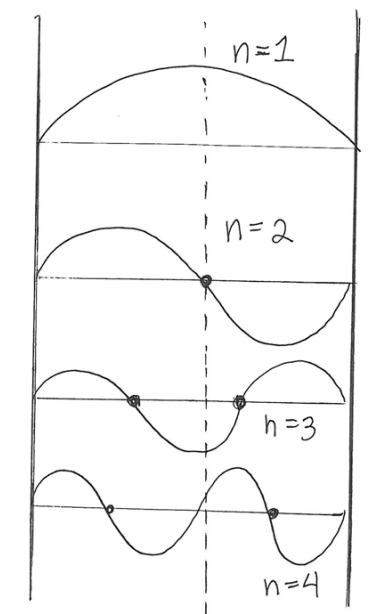
\includegraphics[width=0.5\linewidth]{resources/images/infinite_square_well_eigenstates.png}
    \caption{Graphs of the first four energy eigenstates of the infinite square well centered at $x=0$.}
    \label{infinite_square_well_graph}
\end{figure}

We define a \textbf{node} to be a zero of the wavefunction that is not at an endpoint. Note that the ground state has no nodes. In fact, it is true that any normalizable ground state of a bounded one-dimensional potential has no nodes. Additionally, the $n$th solution $\psi_n$ has $n-1$ nodes. \footnote{See Theorem \ref{node_theorem}.} 

Notice from Figure \ref{infinite_square_well_graph} that the eigenstates alternate even and odd. This is also a general fact: bound states of a symmetric potential $V(x)=V(-x)$ are either odd or even.\footnote{See Corollary \ref{even_potential_cor}.}

Furthermore, we show that all one-dimensional bound states are non-degenerate in energy. Note that this was violated by the particle on a circle because those eigenstates were not bound: the particle was free to traverse the entire real line.

\begin{framedthm}[Non-degeneracy of bound states]\label{non-degeneracy_of_bound_states}
    In any one-dimensional potential $V(x)$, all bound states are non-degenerate in energy.

    \begin{proof}
        Suppose there exist bound states $\psi_1$ and $\psi_2$, both with energy $E$, in the potential $V(x)$. We show that $\psi_1$ and $\psi_2$ must then represent the same state. We have \begin{align*}
            \psi_1''+\frac{2m}{\hbar^2}(E-V)\psi_1&=0\\ \psi_2''+\frac{2m}{\hbar^2}(E-V)\psi_2 &= 0
        \end{align*} 
        Multiplying the first equation by $\psi_2$ and the second by $\psi_1$, 
        \begin{align*}
            \psi_1''\psi_2+\frac{2m}{\hbar^2}(E-V)\psi_1\psi_2&=0\\ \psi_2''\psi_1+\frac{2m}{\hbar^2}(E-V)\psi_2\psi_1 &= 0
        \end{align*} 
        Subtracting the second equation from the first, we have $$\psi_1''\psi_2-\psi_2''\psi_1=0.$$
        By integration by parts, $\int\psi_1''\psi_2=\psi_1'\psi_2-\int\psi_1'\psi_2'$, while $\int\psi_2''\psi_1=\psi_2'\psi_1-\int\psi_2'\psi_1'$. Integrating the above equation\footnote{This integration is possible because $\psi_1$ and $\psi_2$ are bound states, so their integrals do not diverge.} then gives $$\psi_1'\psi_2-\psi_1\psi_2'=0.$$Now recall that from the quotient rule, $$\frac{d}{dx}\bigg(\frac{\psi_1}{\psi_2}\bigg)=\frac{\psi_1'\psi_2-\psi_1\psi_2'}{\psi_2^2}.$$Since we know $\psi_1'\psi_2-\psi_1\psi_2'=0$, we conclude that $\frac{d}{dx}(\frac{\psi_1}{\psi_2})=0$, which implies that $\psi_1=C\psi_2$ for some constant $C$. But then $\psi_1$ and $\psi_2$ are the same state! We conclude that no degenerate bound states exist in one-dimensional potentials.
    \end{proof}
\end{framedthm}

\begin{framedrmk*}
    You might wonder what happens in two or three dimensions. It turns out that degeneracies become incredibly common! You can intuit this by thinking about energy in the classical sense. A one-dimensional particle with a given energy can only behave in one way. However, a two-dimensional particle with a given energy can move in infinitely different ways, depending on the $x$ and $y$ components of its velocity. A similar reasoning applies for quantum mechanical particles constrained to two-dimensional wells.
\end{framedrmk*}

\subsection{The Finite Square Well}\label{finite_square_well}

We next consider the \textbf{finite square well} of height $V_0$ and width $2a$: $$V(x)=
\begin{cases} 
      -V_0 & |x|<a \\
      0& |x|\geq a\\
   \end{cases}$$We will look for bound states, which must have energy $-V_0<E<0$. Otherwise, there would be plane waves propagating infinitely outside the well. For a bound state with energy $E$, the energy $\tilde{E}$ measured from the bottom of the potential is $\tilde{E}=V_0-|E|>0$; these $\tilde{E}$ can be compared with the energies of the infinite square well in the limit as $V_0$ goes to $\infty$.

The time-independent Schrödinger Equation for the finite square well is $$\psi''=\frac{-2m}{\hbar^2}(E-V(x))\psi.$$Let $\alpha(x)=\frac{-2m}{\hbar^2}(E-V(x))$. We consider the two regions separately.

\begin{itemize}
    \item If $|x|\geq a$, $\alpha(x)=\frac{-2m}{\hbar^2}E$ is a positive constant. In this region, the wavefunction is constructed with real exponentials.
    \item If $|x|<a$, $\alpha(x)=\frac{-2m}{\hbar^2}(V_0-|E|)$ is a negative constant. In this region, the wavefunction is constructed with trigonometric functions.
\end{itemize}

We now solve for the energy eigenstates. Note that $V(x)$ is symmetric, and by Corollary \ref{even_potential_cor}, all the bound states must be either odd or even. We deal with these cases separately.

\textbf{Even solutions.} We have $\psi(-x)=\psi(x)$. For $|x|<a$, we have $\psi''=\frac{-2m}{\hbar^2}(V_0-|E|)\psi$. We let $k^2=\frac{2m}{\hbar^2}(V_0-|E|)$, so that $$\psi''=-k^2\psi.$$Since $\psi$ must be even, the solutions are of the form $\psi(x)=\cos kx$, $|x|<a$.

\begin{framedrmk*}[Normalization constants]
    We do not include a normalization constant because we are looking for the possible energy eigenvalues $E$. As long as the wavefunctions are \textit{normalizable}, we do not care what the actual normalization constants are.
\end{framedrmk*}

For $|x|\geq a$, we have $\psi''=\frac{-2m}{\hbar^2}\psi=\frac{2m|E|}{\hbar^2}\psi$. We let $\kappa^2=\frac{2m|E|}{\hbar^2}$, so that $$\psi''=\kappa^2\psi.$$The solutions are of the form $\psi(x)=Ae^{-\kappa x}$, $x\geq a$ (the same thing is mirrored for negative $x$). Note that this time, we do need a normalization constant $A$, in order to ensure we can match the boundary conditions at $x=a$. 

Notice that $k^2$ and $\kappa^2$ satisfy the nice relation $k^2+\kappa^2=\frac{2mV_0}{\hbar^2}$. At this point, we make progress by defining a few unit-free constants.
\begin{align*}\eta&=k a>0,\\ \xi&=\kappa a>0,\\ z_0^2 &=\eta^2+\xi^2=\frac{2mV_0a^2}{\hbar^2}.\end{align*}We are left with a constant $z_0$ that depends on the properties of the potential. A deep, wide potential has large $z_0$, while a shallow, narrow potential has small $z_0$. Importantly, we will see that $z_0$ determines the number of bound states the square well has.

We can also solve for the relations $\frac{|E|}{V_0}=(\frac{\xi}{z_0})^2$ and $\tilde{E}=V_0-|E|=\eta^2\frac{\hbar^2}{2ma^2}$. The first equation gives the energy as a fraction of the depth of the well, while the second equation shows the similarity between the finite well and the infinite well, where the energy states were $E_n=\frac{\hbar^2\pi^2n^2}{2ma^2}$.

The condition that $\psi$ is continuous at $x=a$ yields $$\cos ka=Ae^{-\kappa a}.$$Furthermore, $\psi'$ must be continuous at $x=a$ since $V(x)$ contains no delta functions (See Section \ref{spectrum_continuity_conditions}).  This yields $$-k\sin ka=-\kappa Ae^{-\kappa a}.$$Dividing the second equation by the first gives $k\tan ka=\kappa.$ Multiplying both sides by $a$ to get rid of the units, $$\xi=\eta\tan\eta.$$Finding the even bound states is thus reduced to finding solutions to the equations $\eta^2+\xi^2=z_0^2$ and $\xi=\eta\tan\eta$, where $\eta$ and $\xi$ are both positive. 

The first equation is simply a quarter-circle with radius $r_0$. The second equation is similar in shape to the tangent function. Figure \ref{even_finite_square_well} shows these equations graphed together.

\begin{figure}[H]
    \centering
    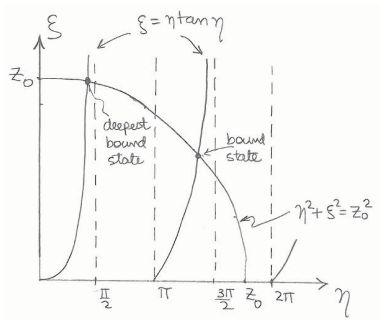
\includegraphics[width=0.5\linewidth]{resources/images/even_finite_square_well.png}
    \caption{A graph of the equations governing the even bound states of the finite square well.}
    \label{even_finite_square_well}
\end{figure}

Since we have $\frac{|E|}{V_0}=(\frac{\xi}{z_0})^2$, the deepest bound state, or the ground state, is the one with the largest $\xi$-coordinate. Note that as $z_0$ grows, it intersects more of the segments of $\xi=\eta\tan\eta$, so that there are more bound states. On the other hand, no matter how small $z_0$ is, there will always be at least one intersection point, representing the existence of at least one bound state

\textbf{Odd solutions.} For odd solutions, keeping all the definitions from above, we have $$\psi(x)=\begin{cases}\sin kx&|x|<a\\Ae^{-k|x|}&|x|>a\end{cases}$$The boundary conditions now give $\xi=-\eta\cot\eta$, and we keep the equation of the circle $\eta^2+\xi^2=z_0^2$. Plotting these curves together, we get Figure \ref{odd_finite_square_well}.

\begin{figure}[H]
    \centering
    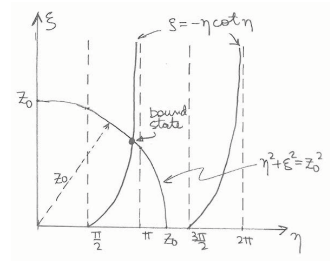
\includegraphics[width=0.5\linewidth]{resources/images/odd_finite_square_well.png}
    \caption{A graph of the equations governing the odd bound states of the finite square well.}
    \label{odd_finite_square_well}
\end{figure}

Note that the curve $\xi=-\eta\cot\eta$ is negative for $\eta<\pi/2$ and thus does not appear in this region. For $z_0<\frac{\pi}{2}$, there are no odd bound state solutions.

Sketches of the first three eigenstates of the finite square well are shown in Figure \ref{finite_well_eigenstates}. They alternate even and odd, and they have successively more nodes.

\begin{figure}
    \centering
    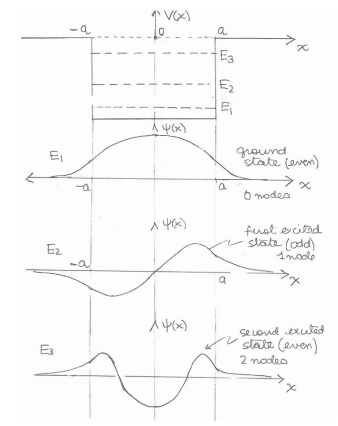
\includegraphics[width=0.5\linewidth]{resources/images/finite_well_eigenstates.png}
    \caption{Sketches of the first three eigenstates of the finite square well.}
    \label{finite_well_eigenstates}
\end{figure}

    \chapter{General Properties}
    \section{Properties of Solutions to the Schrödinger Equation}

\subsection{Real Solutions}\label{real_solutions}

We now take a brief intermission to discuss some general properties of solutions to the Schrödinger equation. First, we can show that $V(x)$ being real allows us to work with real eigenstates.

\begin{framedthm}[Real eigenstates]\label{real_eigenstates}
    The energy eigenstates $\psi(x)$ can be chosen to be real.

    \begin{proof}
        Consider the time-independent Schrödinger equation $$\psi''+\frac{2m}{\hbar^2}(E-V(x))\psi=0.$$Since $(\psi'')^=(\psi^*)''$ and $V(x)$ is real, taking the complex conjugate of the above equation gives $$(\psi^*)''+\frac{2m}{\hbar^2}(E-V(x))\psi^*=0.$$Thus, we see that $\psi^*$ is another solution *with the same energy*. By linearity, we can obtain the real degenerate solutions $$\psi_r=\frac{1}{2}(\psi+\psi^*),\quad\psi_{im}=\frac{1}{2i}(\psi-\psi^*).$$These represent the real and imaginary parts of $\psi$. 
    \end{proof}
\end{framedthm}

Furthermore, if we restrict ourselves to bound states, \textit{all} solutions are real, up to a constant complex phase.

\begin{framedcor}[Real bound states]\label{real_bound_states_cor}

    Any bound state $\psi$ of a one-dimensional potential is real, up to a constant phase.

    \begin{proof} By Theorem \ref{non-degeneracy_of_bound_states}, we know that there are no degenerate bound states in one-dimensional potentials. Thus, the two real solutions $\psi_r$ and $\psi_{im}$ considered above must be equal up to a constant $c\in\mathbb{R}$: $$\psi_{im}(x)=c\psi_r(x).$$It then follows that $\psi=\psi_r+i\psi_{im}=(1+ic)\psi_r$. We can express $1+ic=\sqrt{1+c^2}e^{i\beta}$, which shows that $\psi$ is real up to the constant phase $\beta$. \end{proof}
\end{framedcor}

\subsection{Even Potentials}\label{even_potentials}

Suppose the potential $V(x)$ is even --- that is, it satisfies $V(-x)=V(x)$ for all $x$. It turns out that we can then work with only even and odd wavefunctions.

\begin{framedthm}[Even potentials]\label{even_potential_thm}
    If $V(-x)=V(x)$, the energy eigenstates can be chosen to all be even or odd.

    \begin{proof} Again, we begin with the time-independent Schrödinger equation $$\psi''(x)+\frac{2m}{\hbar^2}(E-V(x))\psi(x)=0.$$We can substitute $-x$ for $x$ to get $$\psi''(-x)+\frac{2m}{\hbar^2}(E-V(x))\psi(-x)=0,$$where we used the fact that $V(x)$ is even. We wish to show that the above equation implies that $\psi(-x)$ is another solution of the Schrödinger equation with the same energy. We define a function $\phi(x)\equiv\psi(-x)$. We see that $$\phi'(x)=-\psi'(x), \text{ and  }\,\phi''(x)=\psi''(-x).$$Thus we have $$\phi''(x)+\frac{2m}{\hbar^2}(E-V(x))\phi(x)=0.$$Therefore, $\phi(x)=\psi(-x)$ is a degenerate solution with the same energy as $\psi$. We can now form the symmetric and antisymmetric combinations $$\psi_s(x)=\frac{1}{2}(\psi(x)+\psi(-x)),\quad\psi_a(x)=\frac{1}{2}(\psi(x)-\psi(-x)).$$These solutions are even and odd, respectively. \end{proof}
\end{framedthm}

Again, if we restrict ourselves to bound states of one-dimensional even potentials, \textit{all} solutions are even or odd.

\begin{framedcor}[Bound states of even potentials]\label{even_potential_cor}
    Any bound state $\psi$ of a one-dimensional even potential is either even or odd.

    \begin{proof}
        Recall from Theorem \ref{non-degeneracy_of_bound_states} that there are no degenerate bound states in one-dimensional potentials. By Corollary \ref{real_bound_states_cor}, $\psi$ is real up to a constant phase, so we must have $$\psi(-x)=c\psi(x)$$for some real constant $c$. Letting $x\rightarrow -x$, we have $\psi(x)=c\psi(-x)=c^2\psi(x)$ from which we see that $c^2=1$. The only possibilities are $c=\pm 1$, so $\psi(x)$ must be even or odd.
    \end{proof}
\end{framedcor}

This result is why we restricted ourselves in Section \ref{finite_square_well} to even and odd bound states. The finite square well is symmetric, and thus cannot have other bound states!

\subsection{The Node Theorem}\label{node_theorem_section}

In Section \ref{nodes_and_symmetries_infinite_square_well}, we noted that the $n$th bound state had $n-1$ nodes. This result is true in general.

\begin{framedthm}[Node theorem]\label{node_thm}
    Given any one-dimensional potential $V(x)$ with bound states $\psi_1,\psi_2,\psi_3,\ldots$ and energy levels $E_1,E_2,E_3,\ldots$, it holds that $\psi_n$ has $(n-1)$ nodes. 
\end{framedthm}

We have seen that Theorem \ref{node_thm} is true for the infinite square well. We now provide an intuitive argument that it holds for any smooth potential $V(x)$ that goes to infinity as $|x|\to\infty$.

Consider an arbitrary such potential. We fix the location $x=0$ at a minimum and define the \textbf{screened potentials} $V_a(x)$ as follows: for any positive real value $a$, we define $$V_a(x)=\begin{cases}V(x)&|x|<a\\\infty&|x|>a \end{cases}$$As shown in Figure \ref{screened}, $V_a(x)$ is an infinite well of width $2a$ whose bottom is $V(x)$.

\begin{figure}
    \centering
    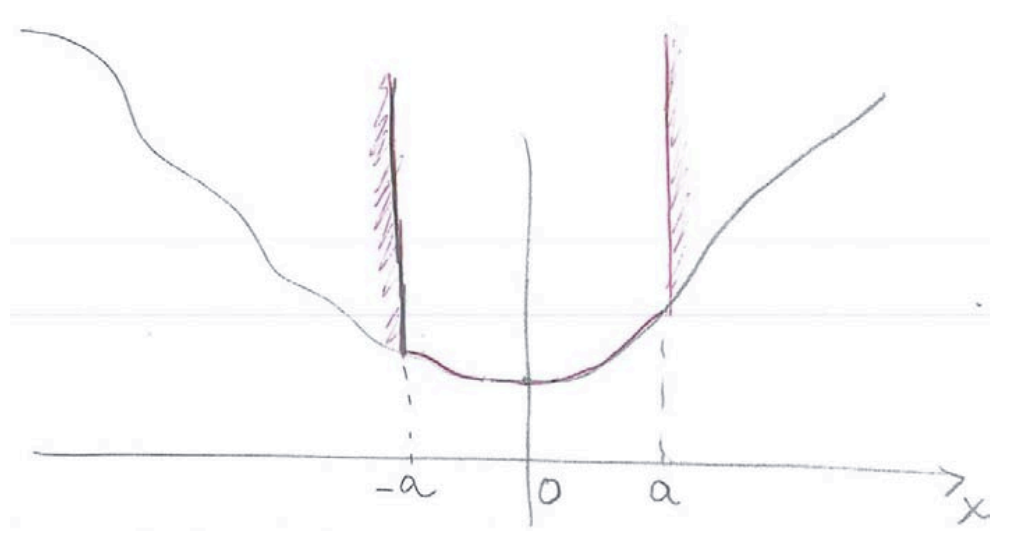
\includegraphics[width=0.5\linewidth]{resources/images/screened.png}
    \caption{The screened potential $V_a(x)$.}
    \label{screened}
\end{figure}

We now take two plausible assumptions. First, as $a$ goes to $\infty$, the bound states of $V_a(x)$ are the bound states of $V(x)$. Additionally, as $a$ increases, the bound states vary continuously.

When $a$ is sufficiently small, $V_a(x)$ can be approximated as a very narrow infinite square well, since we chose $x=0$ to be a minimum and any minimum is locally flat. We know that Theorem \ref{node_thm} holds for this infinite square well. For example, the ground state $\psi$. will have no nodes. We now argue that as $a$ increases, $\psi$ cannot obtain a new node. This argument also holds for all other states.

Suppose a new node is created at $x=a'$ in the potential $V_{a'}(x)$ --- that is, at a boundary of the infinite well. For this to happen, we must have $\psi'(a')>0$, while $\psi'(a)<0$ sufficiently small $a$, as shown in Figure \ref{moving_endpoint}. Assuming continuity, there must be some intermediate screened potential at which $\psi'=0$ at the right endpoint. However, the right endpoint is always the boundary of an infinite well, so $\psi=0$ there. Then we would have $\psi=\psi'=0$ at a point, which would imply that $\psi(x)=0$ for all $x$. This is impossible, so no new nodes can be formed at the boundaries of the well.

\begin{figure}[H]
    \centering
    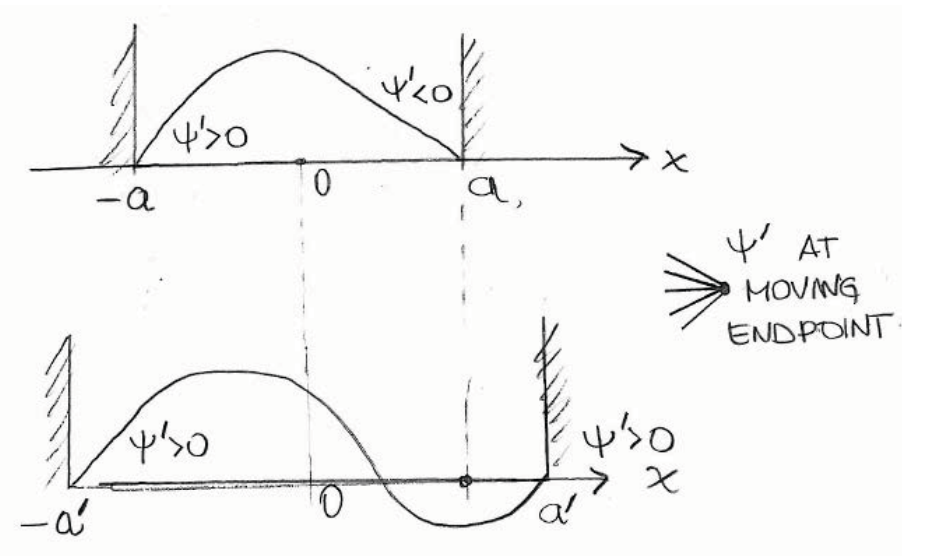
\includegraphics[width=0.5\linewidth]{resources/images/moving_endpoint.png}
    \caption{For sufficiently small $a$, $\psi'(a)<0$. If there exists some $a'$ such that $\psi'(a')>0$, at some point we must have $\psi'=\psi=0$ at the boundary of the well.}
    \label{moving_endpoint}
\end{figure}

We can also imagine introducing a new node at some intermediate point inside the well, so that the sign of $\psi'$ at the endpoints does not change. In this process, shown in Figure \ref{dipping_intermediate}, the wavefunction $\psi$ dips and produces two new nodes. However, this again forces $\psi$ to be tangent to the $x$-axis for some intermediate screen, which is impossible.

\begin{figure}
    \centering
    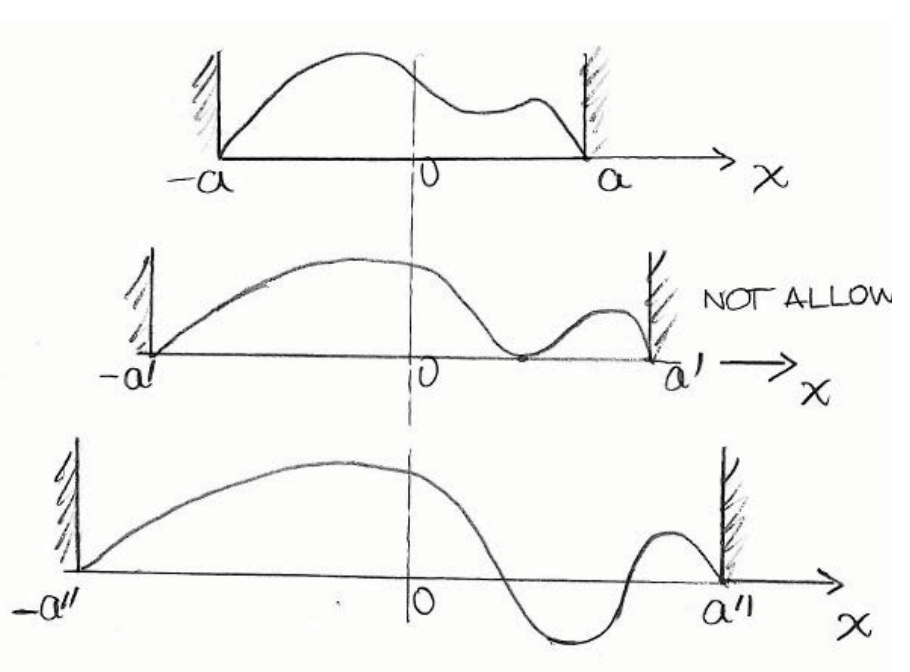
\includegraphics[width=0.5\linewidth]{resources/images/dipping_intermediate.png}
    \caption{If $\psi$ dips below the $x$-axis, there must be an intermediate screen where $\psi$ is tangent to the $x$-axis.}
    \label{dipping_intermediate}
\end{figure}

Since the number of nodes of a wavefunction is constant for all the $V_a(x)$, it must also be the same for $V(x)$. Thus, the node theorem holds for any smooth diverging one-dimensional potential.

\section{The Semi-Classical Approximation}

\subsection{Local de Broglie Wavelength}\label{local_de_broglie}

We will now consider some qualitative insights that classical physics can give us about the behavior of quantum stationary states. This way of thinking is called the \textbf{semi-classical approximation}.

We begin with an example we already understand. Consider the total energy $E$ of a particle as the sum of its potential energy $V$ and its kinetic energy $K$. In our first example, shown in Figure \ref{constant_V}, $V$ is constant. Since $E$ is conserved, $K$ must also be constant. The particle will thus have a constant momentum $p=\sqrt{2mK}$. From Section \ref{deBroglie_proposal}, we know that the wave representing the particle has a de Broglie wavelength $\lambda=\frac{h}{p}$. Indeed, the Schrödinger equation gives $$\psi''=-\frac{2m}{\hbar^2}(E-V)\psi=-\frac{2mK}{\hbar^2}\psi=-\frac{p^2}{\hbar^2}\psi,$$leading to real solutions of the form $$\psi\sim\cos(\frac{p}{\hbar}x)=\cos(\frac{2\pi}{\lambda}x).$$

\begin{figure}
    \centering
    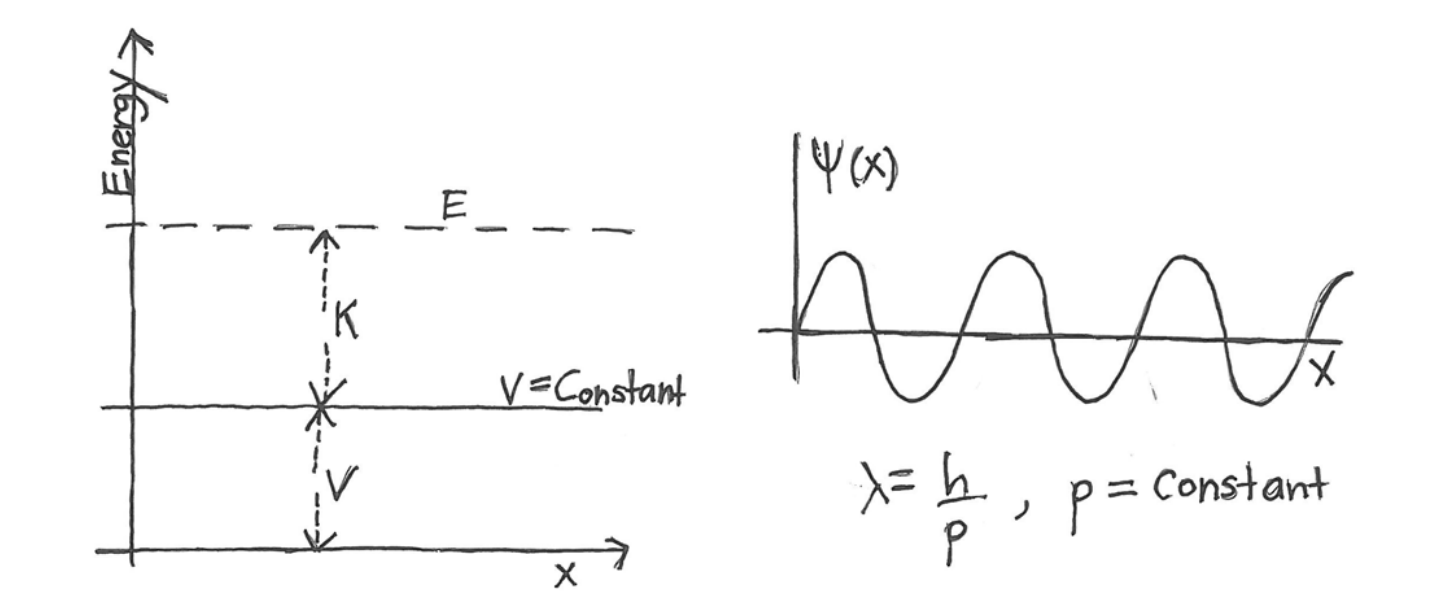
\includegraphics[width=0.5\linewidth]{resources/images/constant_V.png}
    \caption{If $V$ is constant, the particle has constant de Broglie wavelength.}
    \label{constant_V}
\end{figure}

This wavefunction is real and is not a momentum eigenstate; instead, it represents a superposition of a state with momentum $p$ and a state of momentum $-p$. This shouldn't be too surprising; even in the classical case, the kinetic energy only determines $p^2$, and not the sign of $p$.

Consider now the situation depicted in Figure \ref{linearly_increasing_potential}, where we imagine a classical particle moving in a linearly increasing potential $V(x)$. Then the kinetic energy $K(x)$ is also position dependent, and thus so is the momentum $p(x)=\sqrt{2mK(x)}$. As long as the potential is slowly varying, the wavefunction will have a position-dependent de Broglie wavelength approximated by $$\lambda(x)=\frac{h}{p(x)}.$$

\begin{figure}
    \centering
    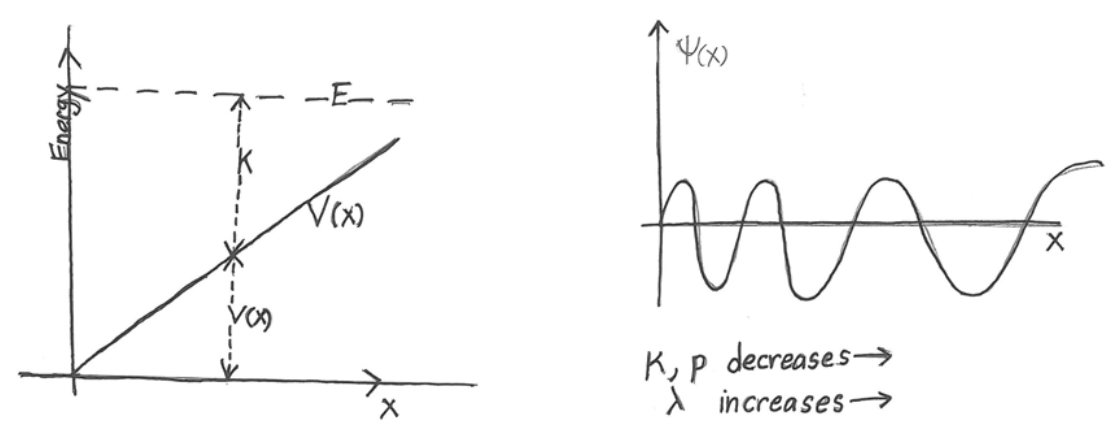
\includegraphics[width=0.5\linewidth]{resources/images/linearly_increasing_potential.png}
    \caption{If $V$ increases, the particle has increasing de Broglie wavelength.}
    \label{linearly_increasing_potential}
\end{figure}

By this we mean that $\psi$ is some combination of functions $$\cos(\frac{2\pi x}{\lambda(x)}),\quad\sin(\frac{2\pi x}{\lambda(x)}).$$This approximation is accurate when the potential changes slowly --- that is, when the change in potential over a distance comparable to the local de Broglie wavelength is very small compared to the potential: $$\lambda(x)\bigg|\frac{dV}{dx}\bigg|\ll |V(x)|.$$

We now draw an arbitrary potential $V(x)$ and consider the classical motion of a particle of total energy $E$. For any point $x_0$, we have $V(x_0)+K(x_0)=E$. The maximum kinetic energy occurs at the minimum value of the potential. The \textbf{forbidden regions} are the regions in which $V(x)>E$, preventing the particle from accessing them. Points where $V(x)=E$ are known as \textbf{turning points}, because the particle must reverse direction at these points.

\begin{figure}
    \centering
    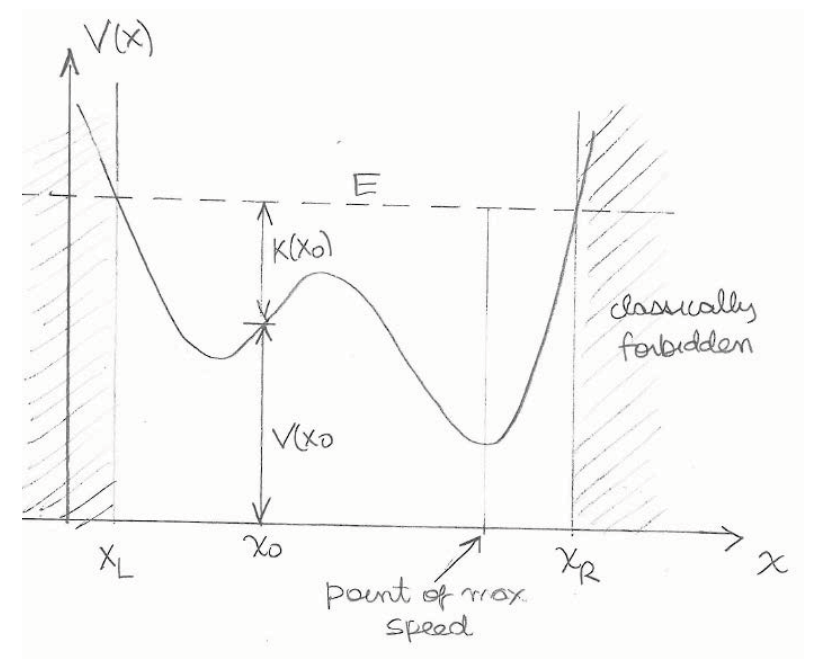
\includegraphics[width=0.5\linewidth]{resources/images/classically_forbidden.png}
    \caption{In the classically forbidden regions, the potential $V(x)$ exceeds the energy $E$ of the particle.}
    \label{classically_forbidden}
\end{figure}

\subsection{The Correspondence Principle}\label{correspondence_principle}

Intuitively, there should be a higher probability of finding the particle in regions where it spends more time. This has significant implications for quantum mechanics.

We already know that the particle is found in a region $dx$ with probability $|\psi|^2dx$. This should also be the fraction of time $\frac{dt}{T}$ that the particle spends in the region. With $v(x)$ the local velocity of the particle, we have that $$|\psi|^2dx\sim\frac{dx}{v(x)T}=\frac{m}{T}\frac{1}{p(x)}dx,$$which implies that the amplitude of the wavefunction is proportional to the square root of the local de Broglie wavelength.

For the linearly increasing potential from Figure \ref{linearly_increasing_potential}, the de Broglie wavelength increases with $x$, so both the amplitude and wavelength of $\psi$ increase with $x$.

\begin{figure}
    \centering
    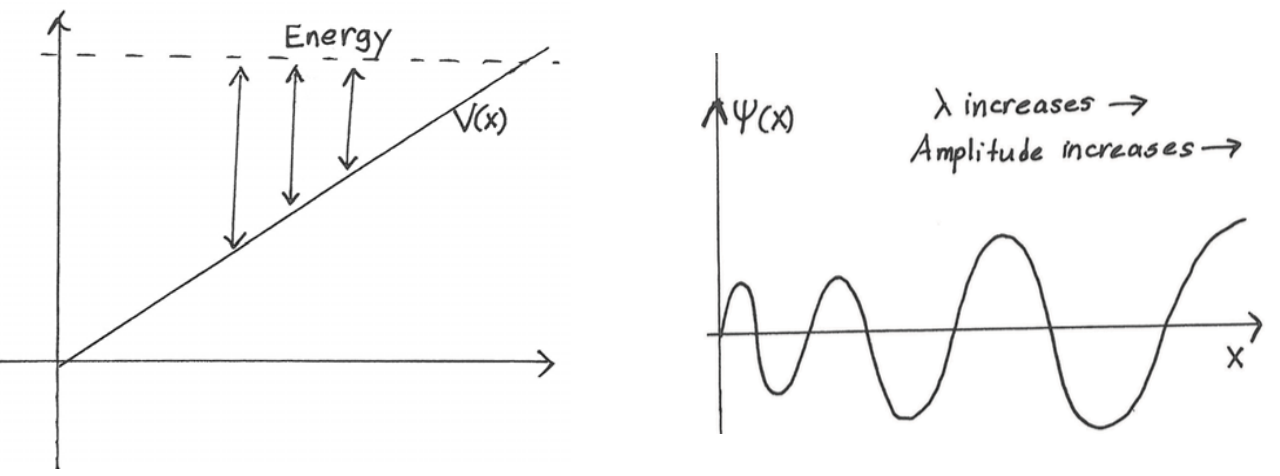
\includegraphics[width=0.5\linewidth]{resources/images/amplitude_increasing.png}
    \caption{In an increasing potential, both the wavelength and amplitude of $\psi$ are increasing.}
    \label{amplitude_increasing}
\end{figure}

For bound states with large energies, averaging $|\psi|$ can be useful to obtain results from classical mechanics. For example, the probability distribution of a particle in an infinite well approaches the classical version when the particle has a very large energy. The idea that there are classical limits of quantum states is called the \textbf{correspondence principle}.

\section{Qualitative Behavior of the Wavefunction}
\subsection{Local Picture of the Wavefunction}\label{local_picture_wavefunction}

From the Schrödinger equation, we have $$\frac{1}{\psi}\frac{d^2\psi}{dx^2}=-\frac{2m}{\hbar^2}(E-V(x)).$$There are three cases for the local behavior of $\psi$.

\begin{enumerate}
    \item The \textbf{classically forbidden region} $E-V(x)<0$. Then the right-hand side of the Schrödinger equation is positive, so either $\psi$ and $\psi''$ are both positive or they are both negative. These possible behaviors are summarized by saying that the wavefunction is \textit{convex towards the axis}. When classically forbidden regions reach to $x=\pm\infty$, the behavior looks like the first sketch in Figure \ref{local_picture}.
    \item The \textbf{classically allowed region} $E-V(x)>0$. Then the right-hand side of the Schrödinger equation is negative, so either $\psi$ is positive and $\psi''$ is negative, or vice versa. This can be summarized by saying that the wavefunction is \textit{concave towards the axis}, as shown in the second skect in Figure \ref{local_picture}. A large classically allowed region has $\psi$ alternating positive and negative, creating a function resembling a sinusoid.
    \item The \textbf{turning points} $E-V(x)=0$. Then we have $\frac{1}{\psi}\psi''=0$, so the turning points are \textit{inflection points} in the graph of $\psi(x)$. Note that not all inflection points are turning points -- in fact, all nodes of the wavefunction are inflection points, since $\psi''=-\frac{2m}{\hbar^2}(E-V(x))\psi=0$ when $\psi(x)=0$. 
\end{enumerate}

\begin{figure}
    \centering
    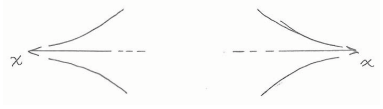
\includegraphics[width=0.4\linewidth]{resources/images/convex.png}
    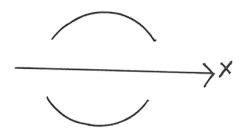
\includegraphics[width=0.4\linewidth]{resources/images/concave.png}
    \caption{When $E-V<0$, the wavefunction looks like the left sketch. When $E-V>0$, the wavefunction looks like the right sketch.}
    \label{local_picture}
\end{figure}

\subsection{Energy Eigenstates on a Generic Symmetric Potential}\label{energy_eigenstates_on_generic_symmetric_potential}

The first sketch in the following diagram displays a smooth, symmetric potential $V(x)$. We wish to see qualitatively why the possible energy levels of bound states in this potential are discrete. The classically forbidden regions must contain $x=\pm\infty$. Without loss of generality, we assume that the end behavior of $\psi$ is positive as $x\rightarrow\infty$, as shown in the top right of Figure \ref{generic_eigenstate}.

\begin{figure}
    \centering
    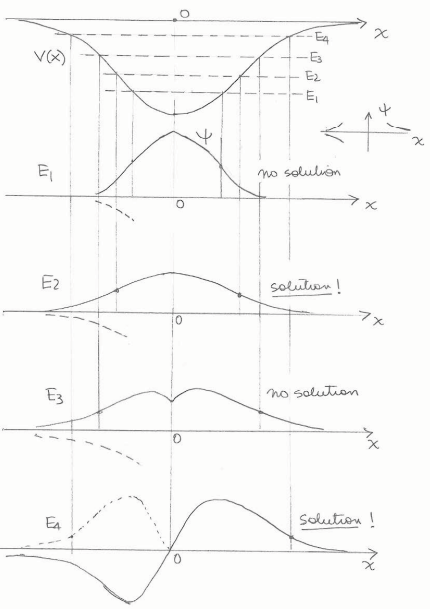
\includegraphics[width=0.7\linewidth]{resources/images/generic_eigenstate.png}
    \caption{Integrating the Schrödinger equation for four energy levels.}
    \label{generic_eigenstate}
\end{figure}

As shown above, we consider the four energies $E_1<E_2<E_3<E_4$, where not all correspond to eigenstates. We imagine integrating the Schrödinger equation from $x=\infty$ to $x=0$ for each value of $E$. 

For example, consider integrating for $E=E_1$. Coming in from $x=\infty$, the solution has an inflection point and becomes concave towards the axis. The same thing happens when coming in from $x=-\infty$. However, the two segments do not match at $x=0$; $\psi'$ fails to be continuous. Thus, $E_1$ is not an allowed energy.

As we increase the energy to $E=E_2$, the turning point occurs for larger and larger $x$, and $\psi'(0)$ is eventually exactly $0$ at $E=E_2$. This represents the ground state of the potential, which is an even solution.

Continuing to increase the energy to $E=E_3$, the turning point becomes even farther away from $x=0$, and $\psi'(0)$ becomes negative. This again cannot be a solution, since $\psi'$ is discontinuous at $x=0$.

Finally, increasing the energy further to some value $E_4$ allows $\psi(0)$ to be exactly $0$. As shown, we can match this to an odd solution. This represents the first excited state of the potential, with a single node at $x=0$.

\subsection{The Shooting Method}\label{shooting_method}

The \textbf{shooting method} is a numerical method to find the form of bound solutions $\psi$ for even potentials $V(x)$. 

We first consider even states. We pick some arbitrary energy $E_0$, and we choose $\psi(0)=1$ since we ignore normalization constants. We must also have $\psi'(0)=0$, since $\psi$ is continuous and even. 

We proceed by integrating the Schrödinger equation numerically. Most likely, $E_0$ will not be an allowed energy value. This will manifest in $\psi$ diverging beyond some value of $x$. Suppose $\psi\rightarrow\infty$. Then we must change the value of the energy until we find some value $E_1$ for which the solution also diverges, but this time with $\psi\rightarrow-\infty$. This is a sign that there is some energy \textit{in between} $E_0$ and $E_1$ for which $\psi$ is normalizable. We then try to narrow this interval, obtaining increasingly better approximations for the actual bound-state energy.

For odd solutions, the procedure is the same, but this time the boundary conditions are $\psi(0)=0$ and $\psi'(0)=1$. The first condition is a requirement for $\psi$ to be odd and continuous, and the second is arbitrary up to normalization.

\begin{framedrmk*}[A practical note]
    When working with computers to carry out these numerical integrations, it is first necessary to clean out the units from the differential equation. That is, we must replace $x$ with a unit-free variable $u$ such that $x=bu$, for some quantity $b$ with units of length built from the parameters in the problem.
\end{framedrmk*}

\section{The Delta Function Potential}

\subsection{Setting Up the Delta Function Potential}\label{setting_up_delta_function}

The \textbf{delta function potential} is an important application of Theorem \ref{node_thm} and the qualitative pictures in Section \ref{energy_eigenstates_on_generic_symmetric_potential}. We consider a particle of mass $m$ moving in the one-dimensional potential $$V(x)=-\alpha\delta(x),$$where $\alpha$ is a positive constant. This potential is shown in Figure \ref{delta_potential_graph}, where the delta function is represented by a downward arrow.

\begin{figure}
    \centering
    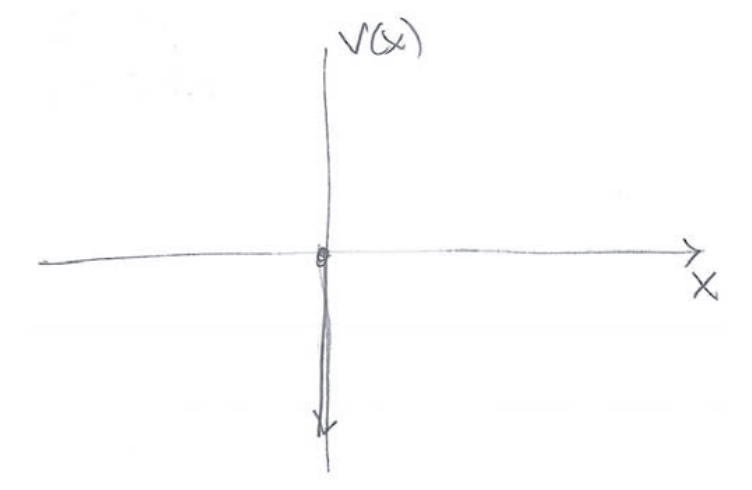
\includegraphics[width=0.5\linewidth]{resources/images/delta_potential.png}
    \caption{A graph of the delta function potential.}
    \label{delta_potential_graph}
\end{figure}

We want to know if this potential admits bound states -- that is, states with energy $E<0$. We gain some intuition by considering units. The dimension-full constants in the problem are $\alpha$, $m$, and $\hbar$. Since a delta function has units of $\frac{1}{L}$, the constant $\alpha$ must have units of energy times length. By dimensional analysis, we see that $$[E]=[\frac{m\alpha^2}{\hbar^2}].$$Therefore, the energy $E_b$ of any bound state must be a negative number times this value: $$E_b=-u\frac{m\alpha^2}{\hbar^2}.$$To find the ground state energy, we only need to find a unit-free number $u$, which we can guess is of order $u \approx 1$.

We can gain further intuition by trying to draw the ground state wavefunction. We can approximate the delta function as a finite square well in the limit of the width going to 0 and the depth going to infinity. As shown in Figure \ref{finite_square_well_limit}, the width of the well provides the curvature needed for the wavefunction to have a continuous derivative. In the limit of an infinitely thin well, the derivative becomes discontinuous at $x=0$.

We now consider the relevant differential equations given by the time-independent Schrödinger equation. For $x\neq 0$, we have $$\psi''=-\frac{2mE}{\hbar^2}\psi=\kappa^2\psi,$$where $\kappa^2=-\frac{2mE}{\hbar^2}>0$. The solutions are of the form $$e^{\kappa x},\,e^{-\kappa x}.$$

\begin{figure}[H]
    \centering
    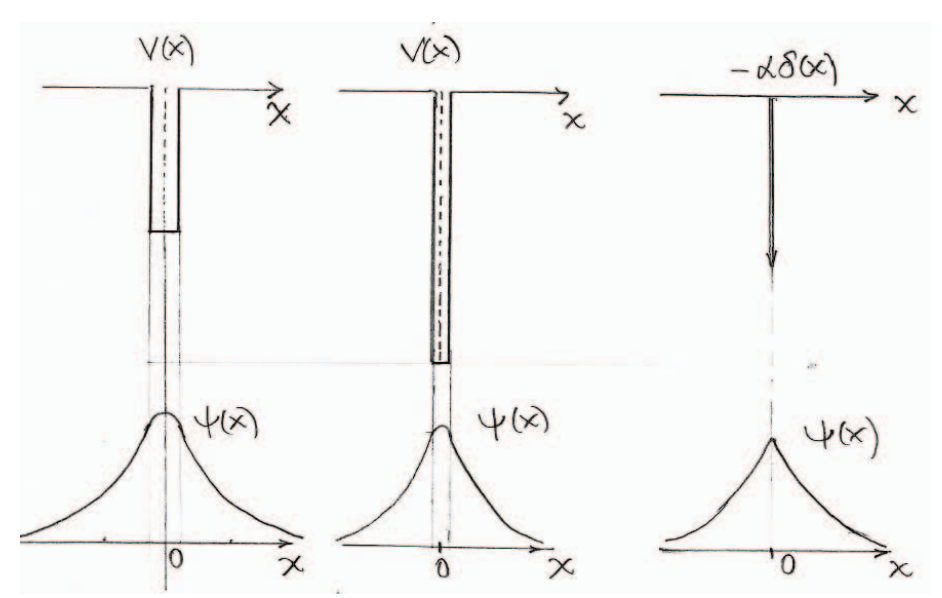
\includegraphics[width=0.5\linewidth]{resources/images/limit_finite_square_wells.png}
    \caption{The delta function potential can be thought of as a finite square well in the limit of width going to $0$ and depth going to $\infty$.}
    \label{finite_square_well_limit}
\end{figure}

Note that the potential is even, so the ground state must be even and have no nodes. The first excited state must then be odd and have a node at $x=0$. However, the only odd solution we can build with the above exponentials is proportional to $$\sinh(\kappa x)\sim e^{\kappa x}-e^{-\kappa x}.$$However, a wavefunction $\psi\sim\sinh(\kappa x)$ certainly cannot be normalized, since it diverges at $x=\pm\infty$. Therefore, there cannot be an excited state in the delta function potential. Without solving anything, we know that if there are bound states, there is just one!

\subsection{Solving the Delta Function Potential}\label{solving_the_delta_potential}

For $\psi$ to be normalizable and continuous, we must have $\psi(x)=Ae^{-\kappa x}$ for $x>0$, and $\psi(x)=Ae^{\kappa x}$ for $x<0$. Thus, the solution must be of the form $$\psi(x)=Ae^{-\kappa|x|}.$$To constrain the possible values of $\kappa$, we rewrite the Schrödinger equation: $$-\frac{\hbar^2}{2m}\psi''+V(x)\psi=E\psi.$$We integrate this equation from $-\epsilon$ to $\epsilon$, with $0<\epsilon\ll 1$, a range that includes the entirety of the delta function. This gives $$-\frac{\hbar^2}{2m}(\frac{d\psi}{dx}\bigg|_\epsilon-\frac{d\psi}{dx}\bigg|_{-\epsilon})+\int_{-\epsilon}^\epsilon dx\,(-\alpha\delta(x))\psi(x)=E\int_{-\epsilon}^\epsilon \psi(x)\,dx.$$In the limit as $\epsilon$ goes to $0$, the integral on the right-hand side vanishes because $\psi(x)$ is finite for all $x$. Meanwhile, the integral of the delta function times $\psi(x)$ simply evaluates $\psi$ at $x=0$, so we have $$-\frac{\hbar^2}{2m}\lim_{\epsilon\to 0}\,(\frac{d\psi}{dx}\bigg|_\epsilon-\frac{d\psi}{dx}\bigg|_{-\epsilon})-\alpha\psi(0)=0.$$We define the \textbf{discontinuity} of $\psi'$ as follows.

\begin{frameddefn}[Discontinuity]
    The \textbf{discontinuity} $\Delta_0$ of $\psi'$ at $x=0$ is $$\Delta_0(\psi')=\lim_{\epsilon\to 0}\,(\frac{d\psi}{dx}\bigg|_\epsilon-\frac{d\psi}{dx}\bigg|_{-\epsilon}).$$As its name suggests, it represents the difference between the slope of the wavefunction just to the right of $x=0$ and just to the left of $x=0$.
\end{frameddefn}

We have now learned that $$\Delta_0(\psi')=-\frac{2m\alpha}{\hbar^2}\psi(0).$$Applying this relation to our solution $\psi(x)=Ae^{-\kappa|x|}$, we have $$\lim_{\epsilon\to 0}(-\kappa Ae^{-\kappa\epsilon}-\kappa Ae^{-\kappa\epsilon})=-2\kappa A=-\frac{2m\alpha}{\hbar^2}A.$$This relation fixes the value of $\kappa$: $$\kappa=\frac{m\alpha}{\hbar^2}.$$Therefore, the bound state energy is $$\boxed{E_b=-\frac{\hbar^2\kappa^2}{2m}=-\frac{1}{2}\frac{m\alpha^2}{\hbar^2}}.$$As we anticipated by dimensional analysis, the answer is proportional to $\frac{m\alpha^2}{\hbar^2}$. The proportionality constant $u$ turns out to be $\frac{1}{2}$.

    \chapter{The Quantum Harmonic Oscillator} 
    \section{Power Series Solution}\label{power_series_solution}
\subsection{Differential Equation}\label{diff_eq_harmonic_oscillator}

The simple harmonic oscillator is an interesting system that allows us to model many complex systems. Classically, the total energy $E$ of a particle of mass $m$ moving in one dimension with a restoring force $F=-kx$ is given by $$E=\frac{p^2}{2m}+\frac{1}{2}m\omega^2x^2,$$where $\omega=\sqrt{\frac{k}{m}}$ is the angular frequency of the oscillations.

\begin{framedrmk*}[Ubiquitousness of the harmonic oscillator]
    Simple harmonic oscillations occur in quadratic potentials. However, \textit{any} potential is approximated as such to first order around a minimum. For example, consider an arbitrary $V(x)$ with a minimum at $x_0$. For $x\approx x_0$, the Taylor expansion of $V(x)$ gives $$V(x)=V(x_0)+(x-x_0)V'(x_0)+\frac{1}{2}(x-x_0)^2V''(x_0)+\mathcal{O}((x-x_0)^3).$$Since $x_0$ is a minimum, $V'(x_0)=0$. Thus, the potential is approximately quadratic for $x\approx x_0$, and small-amplitude oscillations about this point can be approximated with a harmonic oscillator.
\end{framedrmk*}

To define an analogous \textit{quantum} harmonic oscillator, we define the Hamiltonian as $$\hat{H}=\frac{\hat{p}^2}{2m}+\frac{1}{2}m\omega^2\hat{x}^2.$$The harmonic oscillator potential is $$V(x)=\frac{1}{2}m\omega^2x^2.$$We wish to find the energy eigenstates, which will all be bound states since the potential diverges in both directions. There are two methods to solving this system. The first, which we will discuss presently, is a power series solution to the Schrödinger equation. It has the virtue of being applicable to a vast range of potentials. The second, which will be covered in Part \ref{algebraic_solution}, is an ingenious algebraic solution that contains more intuition.

We begin with the analytical method by writing the Schrödinger equation for a state $\phi$: $$-\frac{\hbar^2}{2m}\frac{d^2\phi}{dx^2}+\frac{1}{2}m\omega^2x^2\phi=E\phi.$$As a first step, we change all the constants to be dimensionless. We begin by introducing a unit-free coordinate $u$ to replace the position $x$. We set $x=au$, where $a$ is a constant with units of length. By dimensional analysis, the only combination of $\hbar$, $m$, and $\omega$ with the correct dimensions is $$a=\sqrt{\frac{\hbar}{m\omega}}.$$Substituting $x=au$ into the Schrödinger equation yields $$-\frac{\hbar^2}{2ma^2}\frac{d^2\phi}{du^2}+\frac{1}{2}m\omega^2a^2u^2\phi=E\phi.$$Here, we note that since $\phi$ appears in every term, its units cancel out. Furthermore, since $u$ is dimensionless, we must have $$[\frac{\hbar^2}{ma^2}]=[m\omega^2a^2]=[E].$$Indeed, substituting the value of $a$, we see that both of these quantities equal $\hbar\omega$, which correctly has units of energy. Thus, we have $$-\frac{1}{2}\hbar\omega\frac{d^2\phi}{du^2}+\frac{1}{2}\hbar\omega u^2\phi=E\phi.$$We can even cancel the remaining units by multiplying both sides by $\frac{2}{\hbar\omega}$, which gives $$-\frac{d^2\phi}{du^2}+u^2\phi=\mathcal{E}\phi,$$where we defined the unit-free energy $\mathcal{E}=\frac{E}{\hbar\omega}$. Rearranging, we arrive at a very nice dimensionless form of the Schrödinger equation: $$\boxed{\frac{d^2\phi}{du^2}=(u^2-\mathcal{E})\phi}.$$

\subsection{Recursion Relation}\label{recursion_relation_harmonic_oscillator}

This differential equation surely has solutions for all values of $\mathcal{E}$. Quantization arises because these solutions are not normalizable except for specific values of $\mathcal{E}$. To understand this intuitively, we examine the equation in the limit as $u$ goes to infinity. Then we have $$\lim_{u\to\infty}\phi''(u)= u^2\phi(u).$$Since we want a $u^2$ factor to appear through twice differentiation, we can try an exponential in $u^2$: $$\phi(u)\sim u^ke^{\alpha u^2/2}.$$Then to leading term in $u$, we have $\phi'(u)\approx\alpha u\phi$, and $$\lim_{u\to\infty}\phi''=(\alpha u)^2\phi.$$from which we conclude $\alpha=\pm 1$. Thus, our general solutions for very large $u$ are $$\phi\approx Au^ke^{-u^2/2}+Bu^ke^{u^2/2}.$$The second term diverges as $u\rightarrow\pm\infty$, so we only want the first term. Also, note that the $u^k$ term played no role in the analysis, so we can replace it with an arbitrary polynomial $h(u)$: $$\phi(u)=h(u)e^{-u^2/2}.$$Effectively, we've captured the tendency of the solutions to the Schrödinger equation to diverge in the $e^{-u^2/2}$ term. 

Substituting $\phi(u)$ into the differential equation, we obtain yet another differential equation, this time in $h$: $$\frac{d^2h}{du^2}-2u\frac{dh}{du}+(\mathcal{E}-1)h=0.$$

We can express $h(u)$ as its Taylor series expansion: $$h(u)=\sum_{k=0}^\infty a_ku^k.$$We consider the $u^j$ terms in the differential equation and declare that their coefficient must vanish. The double derivative produces a $(j+2)(j+1)a_{j+2}u^j$ term. Similarly, the second term produces a $-2ja_j$ component, and the last term produces a component of $(\mathcal{E}-1)a_j$. Since the $u^j$ terms must sum to $0$, we have $$(j+2)(j+1)a_{j+2}=(2j+1-\mathcal{E})a_j.$$This is a two-step recursion relation for the Taylor series coefficients $a_k$: $$\boxed{a_{j+2}=\frac{2j+1-\mathcal{E}}{(j+2)(j+1)}a_j}.$$Since this relation skips a step, the value of $a_0$ uniquely defines the even coefficients and thus the even solutions, and $a_1$ defines the odd solutions.
\newpage
\begin{framedrmk*}[Two independent variables]
    Note that $a_0=h(u)$ and $a_1=h'(u)$. It makes sense that we need both $a_0$ and $a_1$ to define $h(u)$, since a specific solution to a second-order differential equation is specified by both the value and derivative of the function at a point.
\end{framedrmk*}

\subsection{Energy Levels and Eigenstates}\label{energy_levels_eigenstates_harmonic_oscillator}

We now show that the Taylor series expansion of $h(u)$ must terminate. Consider the ratio of $a_{j+2}$ to $a_j$ for very large $j$: $$\lim_{j\to\infty}\frac{a_{j+2}}{a_j}\approx\frac{2}{j}.$$Note that $$e^{u^2}=\sum_{n=0}^\infty\frac{1}{n!}u^{2n}=\sum_{j\text{ even}}\frac{1}{(j/2)!}u^j.$$This series has coefficients $c_j=\frac{1}{(j/2)!}$ for even $j$, and we see that as $j$ goes to $\infty$, we have $$\frac{c_{j+2}}{c_j}=\frac{(j/2)!}{(j+2)/2!}=\frac{2}{j+2}\approx\frac{2}{j}.$$ Thus, if $h(u)$ does not terminate, the wavefunction $\phi$ behaves like $$\phi(u)=h(u)e^{-u^2/2}\sim e^{u^2}e^{-u^2/2}= e^{u^2/2},$$which is the diverging solution from before. We conclude that $h(u)$ has some finite degree $j$.

However, recall that we identified a recursion relation for the $a_j$ (boxed on the previous page). For this relation to give $a_j=0$, we must choose $\mathcal{E}$ such that $$2j+1-\mathcal{E}=0.$$This equation quantizes the energy as $$\mathcal{E}=2n+1,\quad n\in\mathbb{N}_0.$$We have $$h(u)=a_nu^n+a_{n-2}u^{n-2}+\ldots$$Since we only have bound states for the harmonic oscillator, Corollary \ref{even_potential_cor} tells us that all solutions are even or odd. If $n$ is odd, we have an odd solution. If $n$ is even, we have an even solution. 

The energy levels are given by $$\boxed{E_n=\hbar\omega(n+\frac{1}{2}).}$$Note that for the harmonic oscillator, the energy levels are evenly spaced with common differences $\hbar\omega$. The corresponding polynomials $h_n(u)$ are called the \textbf{Hermite polynomials}. 

\begin{frameddefn}[Hermite polynomials]
    The Hermite polynomial $H_n(u)$ has leading term $2^nu^n$ by convention and satisfies the differential equation $$\frac{d^2}{du^2}H_n-2u\frac{d}{du}H_n+2nH_n.$$The first few Hermite polynomials are \begin{align*}H_0(u)&=1,\\H_1(u)&=2u,\\H_2(u)&=4u^2-2,\\H_3(u)&=8u^3-12u.\end{align*}The generating function for the Hermite polynomials is an exponential with formal parameter $z$: $$e^{-z^2+2zu}=\sum_{u=0}^\infty\frac{z^n}{n!}H_n(u).$$
\end{frameddefn}

For completeness, we write the energy eigenstates in terms of $x$. Recall that $u^2=\frac{x^2}{a^2}$, where $a^2=\frac{\hbar}{m\omega}$. Thus, we have $$\boxed{\phi_n(x)=N_nH_n\bigg(x\sqrt{\frac{m\omega}{\hbar}}\bigg)e^{-\frac{m\omega}{2\hbar}x^2},}$$where $N_n$ is a normalization constant.

\section{Algebraic Solution}\label{algebraic_solution}
\subsection{Factoring the Hamiltonian}\label{factoring_hamiltonian}

In Part \ref{power_series_solution}, we showed a general analytical solution to the quantum harmonic oscillator that can be applied to a wide variety of potentials. Here, we demonstrate a more elegant approach to the problem. Specifically, we begin by trying to \textit{factor} the Hamiltonian, which we rewrite below: $$\hat{H}=\frac{\hat{p}^2}{2m}+\frac{1}{2}m\omega^2\hat{x}^2=\frac{1}{2}m\omega^2(\hat{x}^2+\frac{\hat{p}^2}{m^2\omega^2}).$$What do we mean by ``factor''? We want to find an operator $\hat{V}$ such that $$H=V^\dagger V+\#.$$Note that $V^\dagger V$ is Hermitian, since $(V^\dagger V)^\dagger=V^\dagger V^{\dagger\dagger}=V^\dagger V$.  The arbitrary constant at the end does not change the properties of the Hamiltonian.

Note that $a^2+b^2=(a-ib)(a+ib)$. Therefore, we consider \begin{align*}(\hat{x}-\frac{i\hat{p}}{m\omega})(\hat{x}+\frac{i\hat{p}}{m\omega})&=\hat{x}^2+\frac{\hat{p}^2}{m^2\omega^2}+\frac{i}{m\omega}(\hat{x}\hat{p}-\hat{p}\hat{x})\\&=\hat{x}^2+\frac{\hat{p}^2}{m^2\omega^2}+\frac{i}{m\omega}[\hat{x},\hat{p}]\\&=\hat{x}^2+\frac{\hat{p}^2}{m^2\omega^2}-\frac{\hbar}{m\omega}.\end{align*}We define $\hat{V}=\hat{x}+\frac{i\hat{p}}{m\omega}$, and since $\hat{x}$ and $\hat{p}$ are Hermitian, we have $\hat{V}^\dagger=\hat{x}-\frac{i\hat{p}}{m\omega}$. We can thus write \begin{align*}\hat{H}&=\frac{1}{2}m\omega^2(V^\dagger V+\frac{\hbar}{m\omega})\\&=\frac{1}{2}m\omega^2V^\dagger V+\frac{1}{2}\hbar\omega.\end{align*}Also note that the commutator of $V$ and $V^\dagger$ is simple: \begin{align*}[V,V^\dagger]&=[\hat{x}+\frac{i\hat{p}}{m\omega},\hat{x}-\frac{i\hat{p}}{m\omega}]=-\frac{i}{m\omega}[\hat{x},\hat{p}]+\frac{i}{m\omega}[\hat{p},\hat{x}].\end{align*}Substituting $[\hat{x},\hat{p}]=i\hbar$, we have $$[V,V^\dagger]=\frac{2\hbar}{m\omega}.$$This implies that $$\bigg[\sqrt{\frac{m\omega}{2\hbar}}V,\sqrt{\frac{m\omega}{2\hbar}}V^\dagger\bigg]=1.$$We now define the unit-free operators $$\hat{a}=\sqrt{\frac{m\omega}{2\hbar}}V,\quad\hat{a}^\dagger=\sqrt{\frac{m\omega}{2\hbar}}V^\dagger.$$For reasons that will become clear later, we call $\hat{a}$ the \textbf{annihilation operator} and $\hat{a}^\dagger$ the \textbf{creation operator}. From the definitions of $V$ and $V^\dagger$ above, we can express $\hat{a}$ and $\hat{a}^\dagger$ in terms of $\hat{x}$ and $\hat{p}$, 
$$\boxed{\hat{a}=\sqrt{\frac{m\omega}{2\hbar}}(\hat{x}+\frac{i\hat{p}}{m\omega}),\quad\hat{a}^\dagger=\sqrt{\frac{m\omega}{2\hbar}}(\hat{x}-\frac{i\hat{p}}{m\omega}),}$$and vice versa:$$\boxed{\hat{x}=\sqrt{\frac{\hbar}{2m\omega}}(\hat{a}+\hat{a}^\dagger),\quad\hat{p}=i\sqrt{\frac{m\omega\hbar}{2}}(\hat{a}^\dagger-\hat{a}).}$$

We now have $$V^\dagger V=\frac{2\hbar}{m\omega}\hat{a}^\dagger\hat{a}.$$Substituting into the Hamiltonian, we get $$\boxed{\hat{H}=\hbar\omega(\hat{a}^\dagger\hat{a}+\frac{1}{2}).}$$We call $\hat{a}^\dagger\hat{a}$ the \textbf{number operator} $\hat{N}$. Since it effectively encodes for the Hamiltonian, it's probably a good idea to figure out how $\hat{N}$ interacts with other operators. We can quickly see that \begin{align*} [\hat{N},\hat{a}]=[\hat{a}^\dagger\hat{a},\hat{a}]=[\hat{a}^\dagger,\hat{a}]\hat{a}=-\hat{a},\\ [\hat{N},\hat{a}^\dagger]=[\hat{a}^\dagger\hat{a},\hat{a}^\dagger]=\hat{a}^\dagger[\hat{a},\hat{a}^\dagger]=\hat{a}^\dagger. \end{align*}Notice that the annihilation operator $\hat{a}$ is accompanied by a negative sign, while the creation operator $\hat{a}^\dagger$ has a positive sign. By induction, we can show that \begin{align*}[\hat{N},(\hat{a})^k]=-k(\hat{a})^k,\\ [\hat{N},(\hat{a}^\dagger)^k]=k(\hat{a}^\dagger)^k.\end{align*}This suggests the reason why $\hat{N}$ is called the number operator: its commutator with some number of creation or annihilation operators is the same operator multiplied by ($\pm$) the number of operators. It almost seems like an eigenvalue equation, where $k$ would be the eigenvalue.

Finally, we note the commutation relations \begin{align*}[\hat{a}^\dagger,(\hat{a})^k]=-k(\hat{a})^{k-1},\\ [\hat{a},(\hat{a}^\dagger)^k]=k(\hat{a}^\dagger)^{k-1}.\end{align*}

\begin{framedrmk*}[Supersymmetric quantum mechanics]
    The process of factorizing the Hamiltonian can be applied to many problems. In fact, there are entire books describing these types of problems, which are grouped together under the field of \textbf{supersymmetric quantum mechanics}.
\end{framedrmk*}

\subsection{Ground State Wavefunction}\label{ground_state_harmonic}

Consider some arbitrary normalized wavefunction $\psi$. We compute the expectation value of $\hat{H}$ on $\psi$: $$\langle\hat{H}\rangle_\psi=(\psi,\hat{H}\psi)=(\psi,\hbar\omega\hat{a}^\dagger\hat{a}\psi+\frac{1}{2}\hbar\omega\psi).$$Splitting the sum, $$\langle\hat{H}\rangle_\psi=\hbar\omega(\psi,\hat{a}^\dagger\hat{a}\psi)+\frac{1}{2}\hbar\omega(\psi,\psi).$$Since $\psi$ is normalized, $(\psi,\psi)=1$. Also, by the definition of the Hermitian conjugate, $(\psi,\hat{a}^\dagger\hat{a}\psi)=(\hat{a}\psi,\hat{a}\psi)$. Thus, we have $$\langle\hat{H}\rangle_\psi=\hbar\omega(\hat{a}\psi,\hat{a}\psi)+\frac{1}{2}\hbar\omega\geq\frac{1}{2}\hbar\omega.$$Here we see the great benefit of the factorized Hamiltonian: since the inner product of any function with itself is nonnegative, we can immediately conclude that every energy eigenstate has energy at least $\frac{1}{2}\hbar\omega$! The minimum energy will be realized for the ground state $\psi_0$ if $(\hat{a}\psi_0,\hat{a}\psi_0)=0$, which implies $$\hat{a}\psi_0=0.$$In other words, the operator $\hat{a}$ \textit{annihilates} the ground state, and is thus called the annihilation operator. From the definition of $\hat{a}$, $$\bigg(x+\frac{i}{m\omega}\frac{\hbar}{i}\frac{d}{dx}\bigg)\psi_0(x)=\bigg(x+\frac{\hbar}{m\omega}\frac{d}{dx}\bigg)\psi_0(x)=0.$$Note that through this process, we have turned a second-order differential equation into a first-order one. Rearranging, $$\frac{d\psi_0}{dx}=-\frac{m\omega}{\hbar}x\psi_0.$$Solving, $$\boxed{\psi_0(x)=\bigg(\frac{m\omega}{\pi\hbar}\bigg)^{\frac{1}{4}}e^{-\frac{m\omega}{2\hbar}x^2}.}$$We can check that $\psi_0$ is an energy eigenstate with energy $E_0=\frac{1}{2}\hbar\omega$: $$\hat{H}\psi_0=\hbar\omega(\hat{a}^\dagger\hat{a}+\frac{1}{2})\psi_0=\frac{1}{2}\hbar\omega\psi_0.$$

\subsection{Excited State Wavefunctions} \label{excited_states_harmonic_oscillator}

We now define the state $\psi_1=\hat{a}^\dagger\psi_0$. This state is an energy eigenstate if it is a number eigenstate, so we consider $$\hat{N}\psi_1=\hat{N}\hat{a}^\dagger\psi_0=[\hat{N},\hat{a}^\dagger]\psi_0,$$because $\hat{a}^\dagger\hat{N}\psi_0=\hat{a}^\dagger\hat{a}^\dagger\hat{a}\psi_0=0$. We have a formula for this commutator: $$\hat{N}\psi_1=[\hat{N},\hat{a}^\dagger]\psi_0=\hat{a}^\dagger\psi_0=\psi_1.$$Thus, $\psi_1$ is a number eigenstate with eigenvalue $1$. It is thus also an energy eigenstate with eigenvalue $E=\hbar\omega(N+\frac{1}{2})=\frac{3}{2}\hbar\omega$.  

We also ask if $\psi_1$ is normalized. We see that$$(\psi_1,\psi_1)=(\hat{a}^\dagger\psi_0,\hat{a}^\dagger\psi_0)=(\psi_0,\hat{a}\hat{a}^\dagger\psi_0)=(\psi_0,[\hat{a},\hat{a}^\dagger]\psi_0)=(\psi_0,\psi_0)=1.$$Thus, $\psi_1$ is automatically normalized as long as $\psi_0$ is. Next consider the state $\psi_2'=\hat{a}^\dagger\hat{a}^\dagger\psi_0=(\hat{a}^\dagger)^2\psi_0$. Again, we operate $\hat{N}$ on $\psi_2'$: $$\hat{N}\psi_2'=\hat{N}(\hat{a}^\dagger)^2\psi_0=[\hat{N},(\hat{a}^\dagger)^2]\psi_0=2(\hat{a}^\dagger)^2=2\psi_2'.$$Thus, $\psi_2'$ is a number eigenstate and also an energy eigenstate, with energy eigenvalue $\frac{5}{2}\hbar\omega$. Again, we try normalizing $\psi_2'$: \begin{align*}(\psi_2'\psi_2') &= (\hat{a}^\dagger\hat{a}^\dagger\,\psi_0,\hat{a}^\dagger\hat{a}^\dagger\,\psi_0)\\ &=(\psi_0,\hat{a}\hat{a}\hat{a}^\dagger\hat{a}^\dagger\,\psi_0) \\ &=(\psi_0,\hat{a}\,[\hat{a},(\hat{a}^\dagger)^2]\,\psi_0) \\ &=(\psi_0,2\hat{a}\hat{a}^\dagger\,\psi_0) \\ &=2(\psi_0,[\hat{a},\hat{a}^\dagger]\,\psi_0)=2.\end{align*}The normalization constant is $\frac{1}{\sqrt{2}}$, so the proper definition of the second excited state is $$\psi_2=\frac{1}{\sqrt{2}}\hat{a}^\dagger\hat{a}^\dagger\psi_0.$$In general, it turns out that $$\boxed{\psi_n=\frac{1}{\sqrt{n!}}(\hat{a}^\dagger)^n\psi_0.}$$The operator $\hat{a}^\dagger$ creates excited states out of the ground state, and is thus called the creation operator. Since they are energy eigenstates with different eigenvalues, the $\psi_n$ are orthonormal: $(\psi_m,\psi_n)=\delta_{mn}$.

Applying the number operator, $$\hat{N}\psi_n=\frac{1}{\sqrt{n!}}\hat{N}(\hat{a}^\dagger)^n\psi_0=\frac{1}{\sqrt{n!}}[\hat{N},(\hat{a}^\dagger)^n]\psi_0=\frac{1}{\sqrt{n!}}n(\hat{a}^\dagger)^n\psi_0=n\psi_n.$$Thus, the $n$th excited state has energy $E=\hbar\omega(n+\frac{1}{2})$. We can also check normalization: $$(\psi_n,\psi_n)=\frac{1}{n!}((\hat{a}^\dagger)^n\psi_0,(\hat{a}^\dagger)^n\psi_0)=\frac{1}{n!}(\psi_0,(\hat{a})^n(\hat{a}^\dagger)^n\psi_0).$$Now consider replacing the last $\hat{a}(\hat{a}^\dagger)^n$ by the commutator $[\hat{a},(\hat{a}^\dagger)^n]=n(\hat{a}^\dagger)^{n-1}$, which we can do because $(\hat{a}^\dagger)^n\hat{a}\psi_0=0$. This brings out a factor of $n$ and gets rid of one factor of $\hat{a}$ and one factor of $\hat{a}^\dagger$. Thus, repeating this process gives us an overall factor of $n!$, making $\psi_n$ normalized.

\subsection{Creation and Annihilation Operators on Energy Eigenstates}\label{creation_annihilation_operators}

We now formalize the effect of $\hat{a}$ and $\hat{a}^\dagger$ on the energy eigenstates. Consider $$\hat{a}\psi_n=\frac{1}{\sqrt{n!}}\hat{a}(\hat{a}^\dagger)^n\psi_0=\frac{1}{\sqrt{n!}}[\hat{a},(\hat{a}^\dagger)^n]\psi_0=\frac{1}{\sqrt{n!}}n(\hat{a}^\dagger)^{n-1}\psi_0.$$By definition, $(\hat{a}^\dagger)^{n-1}\psi_0=\sqrt{(n-1)!}\psi_{n-1}$, so $$\hat{a}\psi_n=\frac{n}{\sqrt{n!}}\sqrt{(n-1)!}\,\psi_{n-1}=\sqrt{n}\,\psi_{n-1}.$$Similarly, we have $$\hat{a}^\dagger\psi_n=\frac{1}{\sqrt{n!}}(\hat{a}^\dagger)^{n+1}\psi_0=\frac{1}{\sqrt{n!}}\sqrt{(n+1)!}\,\psi_{n+1}=\sqrt{n+1}\,\psi_{n+1}.$$Collecting the results, we have We now formalize the effect of $\hat{a}$ and $\hat{a}^\dagger$ on the energy eigenstates. Consider $$\hat{a}\psi_n=\frac{1}{\sqrt{n!}}\hat{a}(\hat{a}^\dagger)^n\psi_0=\frac{1}{\sqrt{n!}}[\hat{a},(\hat{a}^\dagger)^n]\psi_0=\frac{1}{\sqrt{n!}}n(\hat{a}^\dagger)^{n-1}\psi_0.$$By definition, $(\hat{a}^\dagger)^{n-1}\psi_0=\sqrt{(n-1)!}\psi_{n-1}$, so $$\hat{a}\psi_n=\frac{n}{\sqrt{n!}}\sqrt{(n-1)!}\,\psi_{n-1}=\sqrt{n}\,\psi_{n-1}.$$Similarly, we have $$\hat{a}^\dagger\psi_n=\frac{1}{\sqrt{n!}}(\hat{a}^\dagger)^{n+1}\psi_0=\frac{1}{\sqrt{n!}}\sqrt{(n+1)!}\,\psi_{n+1}=\sqrt{n+1}\,\psi_{n+1}.$$Collecting the results, we have
\begin{align*}
\hat{a}\psi_n&=\sqrt{n}\,\psi_{n-1},\\ \hat{a}^\dagger\psi_n &= \sqrt{n+1}\,\psi_{n+1}.
\end{align*}
These relations make it clear that the annihilation operator decreases the number of an energy eigenstate, while the creation operator increases the number.

\begin{framedexpl}[Expectation values in a harmonic oscillator]
    Find the expectation values of $\hat{x}$ and $\hat{p}$ in the state $\psi_n$.
\end{framedexpl}

\begin{framedansw*}
    Consider the value $\langle\hat{x}\rangle_{\psi_n}=\int x\psi_n(x)^2 dx$. Since the potential is even, $\psi_n$ is either even or odd. Either way, $\psi_n^2$ is even. However, $x$ is odd, so the integral cancels out and we have $\langle\hat{x}\rangle_{\psi_n}=0$.

    It's also worth it to consider this expectation value using the creation and annihilation operators. By definition, we have $\hat{x}=\sqrt{\frac{\hbar}{2m\omega}}(\hat{a}+\hat{a}^\dagger)$. Thus, we have $$\langle\hat{x}\rangle=(\psi_n,\hat{x}\psi_n)=\sqrt{\frac{\hbar}{2m\omega}}(\psi_n,(\hat{a}+\hat{a}^\dagger)\psi_n).$$As we found above, the second term is $\sqrt{n}\,\psi_{n-1}+\sqrt{n+1}\,\psi_{n+1}$. Thus, $\langle\hat{x}\rangle\sim(\psi_n,\psi_{n-1})+(\psi_n,\psi_{n+1})=0$.

    Furthermore, note that $\psi_n$ is a stationary state. Thus, the expectation value of $x$ must be time-independent, so there can be no expected momentum. We conclude that $\langle\hat{p}\rangle_{\psi_n}=0$ also.
\end{framedansw*}

\begin{framedexpl}[Uncertainty in a harmonic oscillator]
    Find the position uncertainty $\Delta x$ in $\psi_n$.
\end{framedexpl}

\begin{framedansw*}
    We have $(\Delta x)^2=\langle\hat{x}^2\rangle-\langle\hat{x}\rangle^2=\langle\hat{x}^2\rangle$, since the second term goes to $0$.

    Expanding, we see that \begin{align*}\langle\hat{x}^2\rangle&=(\psi_n,(\hat{x})^2\psi_n)\\ &=\frac{\hbar}{2m\omega}(\psi_n,(\hat{a}+\hat{a}^\dagger)^2\psi_n)\\ &=\frac{\hbar}{2m\omega}(\psi_n,(\hat{a}\hat{a}^\dagger+\hat{a}^\dagger\hat{a}^\dagger+\hat{a}\hat{a}^\dagger+\hat{a}^\dagger\hat{a})\psi_n).\end{align*}Note that the $\hat{a}\hat{a}$ and $\hat{a}^\dagger\hat{a}^\dagger$ terms result in the wrong number eigenstate, so the inner product of these states with $\psi_n$ is $0$. This leaves $$\langle\hat{x}^2\rangle=\frac{\hbar}{2m\omega}(\psi_n,(\hat{a}\hat{a}^\dagger+\hat{a}^\dagger\hat{a})\psi_n]).$$Furthermore, note that $\hat{a}^\dagger\hat{a}=\hat{N}$. The other order, $\hat{a}\hat{a}^\dagger$, can be written as $[\hat{a},\hat{a}^\dagger]+\hat{a}^\dagger\hat{a}=1+\hat{N}$. Therefore, we have $$\langle\hat{x}^2\rangle=\frac{\hbar}{2m\omega}(\psi_n,(1+2\hat{N})\psi_n)=\frac{\hbar}{2m\omega}(\psi_n,\psi_n)(1+2n).$$Our final result is $$\boxed{(\Delta x)^2=\langle\hat{x}^2\rangle_{\psi_n}=\frac{\hbar}{m\omega}(n+\frac{1}{2}).}$$
\end{framedansw*}

    \chapter{Scattering States}
    \section{The Step Potential}
\subsection{Energy Above the Barrier}\label{energy_above_barrier}

We now begin our study of \textbf{scattering states}. These are energy eigenstates that cannot be normalized:

\begin{frameddefn}[Scattering states]
    A scattering state is an energy eigenstate that cannot be normalized.
\end{frameddefn}

Similarly to the plane waves we considered earlier, these do not represent physical states of a particle. Instead, we must consider superpositions of these states for them to have physical meaning.

We begin by considering the \textbf{step potential} $$V(x)=\begin{cases}0 & x<0 \\ V_0 & x\geq 0\end{cases}$$There are two cases: $E>V_0$ and $E<V_0$. In both cases, the wavefunction extends infinitely to the left and is non-normalizable. In this section, we consider the case $E>V_0$, as depicted in Figure \ref{step_e_bigger}.

\begin{figure}
    \centering
    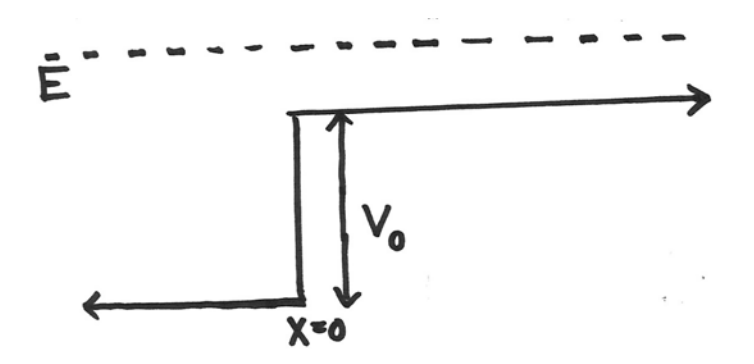
\includegraphics[width=0.5\linewidth]{resources/images/step_e_bigger.png}
    \caption{A sketch of the step potential for $E>V_0$.}
    \label{step_e_bigger}
\end{figure}

To find $\psi(x)$, we imagine a physical process in which a wave $Ae^{ikx}$ is incident on the step from the left. We would expect a reflected wave $Be^{-ikx}$ moving to the left from the step and a transmitted wave $Ce^{i\bar{k}x}$ moving to the right: $$\psi(x)=\begin{cases}Ae^{ikx}+Be^{-ikx}&x<0 \\ Ce^{i\bar{k}x}&x>0\end{cases}$$We can obtain the wavenumbers $k$ and $\bar{k}$ via the Schrödinger equation: $$k^2=\frac{2mE}{\hbar^2},\quad\bar{k}^2=\frac{2m(E-V_0)}{\hbar^2}.$$Furthermore, both $\psi$ and $\psi'$ must be continuous at $x=0$; these boundary conditions constrain the values of $A$, $B$, and $C$. Continuity of $\psi$ gives $A+B=C$, and continuity of $\psi'$ gives $ikA-ikB=i\bar{k}C$. Rearranging, $A-B=\frac{\bar{k}}{k}C$. Solving for $B$ and $C$ in terms of $A$, we get $$\frac{B}{A}=\frac{k-\bar{k}}{k+\bar{k}},\quad\frac{C}{A}=\frac{2k}{k+\bar{k}}.$$This is the best we can do; the value of the independent variable $A$ can be thought of as the \textit{input}, since it defines the amplitude of the incoming wave. Mathematically, it represents a normalization factor.

In the limit as $E\to V_0$, we have $\bar{k}\to 0$, so $B=A$ and $C=2A$. Then the solution is $$\psi(x)=\begin{cases}2A\cos(kx)&x<0 \\ 2A&x>0\end{cases}$$This wavefunction is shown in Figure \ref{e_bigger_v_wavefunction}.

\begin{figure}[H]
    \centering
    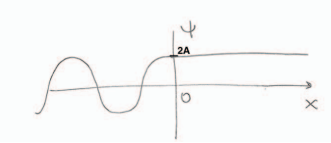
\includegraphics[width=0.5\linewidth]{resources/images/e_bigger_v_wavefunction.png}
    \caption{A sketch of the wavefunction in the limit as $E\to V_0$.}
    \label{e_bigger_v_wavefunction}
\end{figure}

We can obtain further insight by evaluating the probability current just to the left and the right of the step. Recall from Theorem \ref{current_conservation_thm} that the probability current $J$ for a wavefunction $\psi$ is $$J=\frac{\hbar}{m}\operatorname{Im}(\psi^*\frac{\partial\psi}{\partial x}).$$A short calculation shows that the current $J_L$ to the left of the step is $$J_L=\frac{\hbar k}{m}(|A|^2-|B|^2)=J_A-J_B,$$where $J_A=\frac{\hbar k}{m}|A|^2$ and $J_B=\frac{\hbar k}{m}|B|^2$. Note that there is no interference between the incident and reflected waves; the total current to the left of the step is simply the incident wave current minus the reflected wave current. Similarly, the current $J_R$ to the right of the step is $$J_R=\frac{\hbar \bar{k}}{m}|C|^2=J_C.$$Note that both $J_L$ and $J_R$ are time-independent. Thus, current conservation requires $J_L=J_R$ -- the current must be independent of position. We check that \begin{align*}J_L &=\frac{\hbar k}{m}(|A|^2-|B|^2) \\ &=\frac{\hbar k}{m}(1-(\frac{k-\bar{k}}{k+\bar{k}})^2)|A|^2 \\ &= \frac{\hbar k}{m}(\frac{4k\bar{k}}{(k+\bar{k})^2})|A|^2 \\ &=\frac{\hbar \bar{k}}{m}\frac{4k^2}{(k+\bar{k})^2}|A|^2=\frac{\hbar k}{m}|C|^2=J_R.\end{align*}

\subsection{Reflection and Transmission Coefficients}\label{reflection_transmission_coefficients}

However, since the incident and reflected waves do not interfere, current conservation gives us $J_A-J_B=J_C$. Rearranging, $$1=\frac{J_B}{J_A}+\frac{J_C}{J_A}.$$We define the \textbf{reflection coefficient} $R$ as the ratio of the probability flux due to the reflected wave to that of the incident wave: $$R=\frac{J_B}{J_A}=\frac{|B|^2}{|A|^2}=(\frac{k-\bar{k}}{k+\bar{k}})^2\leq 1.$$Similarly, we define the \textbf{transmission coefficient} $T$ as the ratio of the probability flux due to the transmitted wave to that of the incident wave: $$T=\frac{J_C}{J_A}=\frac{\bar{k}}{k}\frac{|C|^2}{|A|^2}=\frac{\bar{k}}{k}\frac{4k^2}{(k+\bar{k})^2}=\frac{4k\bar{k}}{(k+k^2)}.$$We therefore have $$R+T=1.$$Note that the wavelengths to the left and right of the step are different, so $T\neq \frac{|C|^2}{|A|^2}$.

Recall that for $E=V_0$ we have $\bar{k}=0$. Then we have full reflection: $R=1$ and $T=0$. Indeed, the probability current associated with the constant wavefunction that exists for positive $x$ is zero.

\subsection{Energy Below the Barrier}\label{e_less_v_step}

We now consider the case when $E<V_0$, as depicted in Figure \ref{step_e_smaller}.

\begin{figure}
    \centering
    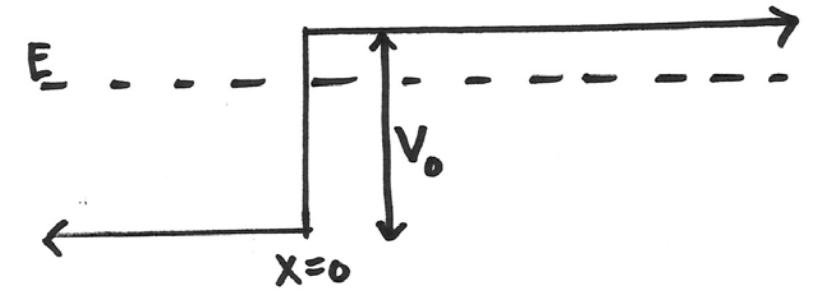
\includegraphics[width=0.5\linewidth]{resources/images/step_e_smaller.png}
    \caption{A sketch of the step potential for $E<V_0$.}
    \label{step_e_smaller}
\end{figure}

Now the region $x>0$ is classically forbidden. Let us try to solve for the energy eigenstate without redoing all the work we have already done in finding $B$ and $C$ in terms of $A$. Note that for $x<0$, the solution is unchanged and we still have $$\psi(x)=Ae^{ikx}+Be^{-ikx},\quad x<0$$ for $k^2=\frac{2mE}{\hbar^2}$. On the other hand, for $x>0$, the earlier solution $\psi(x)=C e^{i\bar{k}x}$ should become a decaying exponential $\psi(x)=C e^{-\kappa x}$ for $\kappa^2=\frac{2m(V_0-E)}{\hbar^2}$. Note that the former becomes the latter upon replacing $\bar{k}$ with $i\kappa$.

Therefore, we can simply perform this replacement in our earlier expressions for $B/A$ and $C/A$. In particular, we have $$\frac{B}{A}=\frac{k-i\kappa}{k+i\kappa}=\frac{i(k-i\kappa)}{i(k+i\kappa)}=-\frac{\kappa+ik}{\kappa-ik}=-e^{2i\delta(E)}$$with $$\delta(E)=\tan^{-1}(\frac{k}{\kappa})=\tan^{-1}(\sqrt{\frac{E}{V_0-E}}).$$Since the magnitude of $A$ is equal to the magnitude of $B$, we have $J_A=J_B$ and $J_C=0$. Thus, $T=0$ and $R=1$. As noted above, the ratio $\frac{B}{A}$ is a pure phase, and $\delta(E)\to 0$ as $E\to 0$. Note that $\delta(E)$ is positive and does not exceed $\pi/2$. A sketch of $\delta(E)$ is shown in Figure \ref{delta_step}.

\begin{figure}
    \centering
    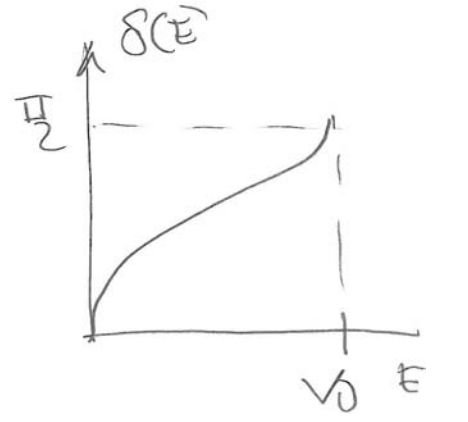
\includegraphics[width=0.5\linewidth]{resources/images/delta_step.png}
    \caption{A graph of $\delta(E)=\tan^{-1}(\sqrt{\frac{E}{V_0-E}})$.}
    \label{delta_step}
\end{figure}

The total wavefunction is $$\psi(x)=\begin{cases}Ae^{ikx}-Ae^{2i\delta(E)}e^{-ikx}&x<0 \\ Ce^{-\kappa x} & x>0\end{cases}$$For $x<0$, the wavefunction takes an interesting form: \begin{align*}\psi(x)&=Ae^{i\delta(E)}(e^{kx-\delta(E)}-e^{-i(kx-\delta(E))})\\ &= 2iAe^{i\delta(E)}\sin(kx-\delta(E)).\end{align*}Thus, the probability density is $$|\psi|^2=4A^2\sin^2(kx-\delta(E)).$$The point $x_0=\frac{\delta(E)}{k}>0$ in Figure \ref{step_e_smaller_wavefunction} is the point in the classically forbidden region where the extrapolation of the allowed-region solution would vanish. Of course, the probability density in the forbidden region is actually a decaying exponential. 

\begin{figure}[H]
    \centering
    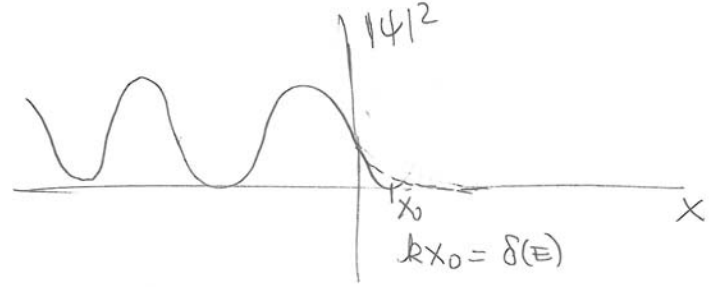
\includegraphics[width=0.5\linewidth]{resources/images/step_e_smaller_wavefunction.png}
    \caption{A sketch of the probability amplitude in the allowed and forbidden regions. At $x_0$, the forbidden region wavefunction is $0$, but the actual wavefunction is nonzero.}
    \label{step_e_smaller_wavefunction}
\end{figure}
For future use, we write the derivative of the phase $\delta(E)$: $$\delta'(E)=\frac{1}{2}\sqrt{\frac{1}{E(V_0-E)}}.$$This derivative becomes infinite for both $E\to 0$ and $E\to V_0$.

\subsection{Particle in the Forbidden Region}\label{particle_in_forbidden_region}

The fact that the wavefunction is nonzero in the forbidden region seems like it could lead to problems. Note that it would be contradictory if the observer could make both of the following two statements.

\begin{enumerate}
    \item The particle is located in the forbidden region.
    \item The particle has energy less than $V_0$. 
\end{enumerate}

If both statements were to hold simultaneously, the particle would have to have negative kinetic energy, which is impossible. How can we resolve this apparent contradiction? By invoking the uncertainty principle from Section \ref{widths_uncertainties}.

First note that in the forbidden region, the particle is governed by an exponentially decaying wavefunction of order $e^{-\kappa x}$. This implies that the particle penetrates a distance of approximately $\frac{1}{\kappa}$, where $$\kappa^2=\frac{2m(V_0-E)}{\hbar^2}.$$To be sure the particle is in the forbidden region, its position uncertainty $\Delta x$ must be smaller than the penetration depth: $$\Delta x\leq \frac{1}{\kappa}.$$By the uncertainty principle, the particle must have some momentum uncertainty $$\Delta p\geq \frac{\hbar}{\Delta x}\geq\hbar\kappa.$$Now there must be some uncertainty in kinetic energy $$\Delta KE=\frac{(\Delta p)^2}{2m}\geq \frac{\hbar^2\kappa^2}{2m}=V_0-E.$$Thus, given the first statement above, the second statement cannot be made! The very act of observing the particle in the forbidden region creates just enough uncertainty in the kinetic energy to make the total energy $V_0$. 

\section{Wavepackets on the Step Potential}

\subsection{Wavepackets with Energy Above the Barrier}\label{wavepackets_energy_above_barrier}

We now consider the physical states. As we've seen with the free particle in Section \ref{free_particle}, the stationary states are not normalizable. Instead, physical states are represented by wavepackets built from an infinite superposition of eigenstates. In this section, we will consider wavepackets built from energy eigenstates with $E>V_0$, or equivalently, $k^2>\hat{k}^2$, where $$k^2=\frac{2mE}{\hbar^2}>\frac{2mV_0}{\hbar^2}=\hat{k}^2.$$To begin with, we write the energy eigenstates including the time dependence. Let the wave be incident on the barrier at $t=0$. Setting $A=1$, we have $$\Psi(x,t)=\begin{cases}(e^{ikx}+\frac{k-\bar{k}}{k+\bar{k}}e^{-ikx})e^{-iE(k)t/\hbar} & x<0 \\ \frac{2k}{k+\bar{k}}e^{i\bar{k}x}e^{-iE(k)t/\hbar} & x>0\end{cases}$$We can form a superposition of these solutions by multiplying by a function $f(k)$ and integrating over $k$: 
$$\Psi(x,t)=\begin{cases}\int_{\hat{k}}^\infty dk\,f(k)(e^{ikx}+\frac{k-\bar{k}}{k+\bar{k}}e^{-ikx})e^{-iE(k)t/\hbar} & x<0 \\ \int_{\hat{k}}^\infty dk\,f(k)\frac{2k}{k+\bar{k}}e^{i\bar{k}x}e^{-iE(k)t/\hbar} & x>0\end{cases}$$
Here $f(k)$ is a real function of $k$ that is essentially zero except for a narrow peak at $k=k_0$. Note that we have only included momentum components with energy greater than $V_0$ by setting the lower bound of the integral to $\hat{k}$. The integral only ranges over positive $k$ because only in that case are the incident $e^{ikx}$ waves moving to the right. Since $\Psi$ is the superposition of eigenstates multiplied by a number $f(k)$, it is guaranteed to be a solution of the Schrödinger equation.

We can split the solution into incident, reflected, and transmitted waves: $$\Psi(x,t)=\begin{cases}\Psi_{inc}(x,t)+\Psi_{ref}(x,t) & x<0 \\ \Psi_{trans}(x,t) & x>0\end{cases}$$Of course, both $\Psi_{inc}$ and $\Psi_{ref}$ exist only for negative $x$, while $\Psi_{trans}$ exists only for positive $x$. We then have \begin{align*}\Psi_{inc}(x<0,t)&=\int_{\hat{k}}^\infty dk\,f(k)e^{ikx}e^{-iE(k)t/\hbar}, \\ \Psi_{ref}(x<0,t)&=\int_{\hat{k}}^\infty dk\,f(k)\frac{k-\bar{k}}{k+\bar{k}}e^{-ikx}e^{-iE(k)t/\hbar}, \\ \Psi_{trans}(x>0,t)&=\int_{\hat{k}}^\infty dk\,f(k)\frac{2k}{k+\bar{k}}e^{i\bar{k}x}e^{-iE(k)t/\hbar}.\end{align*}How does the peak of $\Psi_{inc}(x,t)$ move? To answer this question, we use the stationary phase approximation. Recall from Theorem \ref{principle_stationary_phase} that the main contribution to the integral occurs when the total phase in the integrand is stationary for $k\approx k_0$: $$\frac{d}{dk}(kx-\frac{\hbar^2k^2}{2m}\frac{t}{\hbar})\bigg|_{k_0}=0\implies x-\frac{\hbar k_0}{m}t=0.$$This is the relation between $t$ and $x$ satisfied by the peak of $\Psi_{inc}$. It describes a peak moving with constant positive velocity $\frac{\hbar k_0}{m}>0$. Since $\Psi_{inc}(x,t)$ requires that $x<0$, we only get a peak for $t<0$. For positive $t$, the stationary phase condition cannot be satisfied for any $x<0$, so $\Psi_{inc}(x,t)$ becomes negligible.

Now consider $\Psi_{ref}(x,t)$. This time, the stationary phase condition gives $$\frac{d}{dk}(-kx-\frac{\hbar^2 k^2}{2m}\frac{t}{\hbar})\bigg|_{k_0}=0\implies x+\frac{\hbar k_0}{m}t=0.$$This relation represents a peak moving with constant negative velocity $\frac{-\hbar k_0}{m}$. Since $\Psi_{ref}(x,t)$ requires that $x<0$, we only get a peak for $t>0$. This is intuitive, since the wave only reflects at $t=0$. For negative $t$, the stationary phase condition cannot be satisfied for any $x>0$, so $\Psi_{ref}(x,t)$ is negligible.

Finally, we consider $\Psi_{trans}(x,t)$. We have $$\frac{d}{dk}(\bar{k}x-\frac{\hbar^2k^2}{2m}\frac{t}{\hbar})\bigg|_{k_0}=0\implies \frac{d\bar{k}}{dk}\bigg|_{k_0}x-\frac{\hbar k_0}{m}t=0.$$From implicit differentiation using $\bar{k}^2=k^2-\frac{2mV_0}{\hbar^2}$, we know that $\frac{d\bar{k}}{dk}=\frac{k}{\bar{k}}$. Thus, we have $$\frac{k_0}{\bar{k}}x-\frac{\hbar k_0}{m}t=0\implies x=\frac{\hbar\bar{k}}{m}t.$$This relation represents a peak moving with constant positive velocity $\frac{\hbar\bar{k}}{m}$. Since $\Psi_{trans}(x,t)$ requires that $x>0$, we only get a peak for $t>0$. Again, this is intuitive, since the wave is only transmitted at $t=0$. For negative $t$, the stationary phase condition cannot be satisfied for any $x>0$, so $\Psi_{trans}(x,t)$ is negligible. 

\begin{framedrmk*}[Summary]
    For large negative times, $\Psi_{inc}$ dominates and both $\Psi_{ref}$ and $\Psi_{trans}$ are very small. For large positive times, both $\Psi_{ref}$ and $\Psi_{trans}$ dominate and $\Psi_{inc}$ is very small. These solutions are shown in Figure \ref{step_potential_solution_sketch}. For times close to $t=0$, all three waves exist and together describe the complex collision process.
\end{framedrmk*}

\begin{figure}[H]
    \centering
    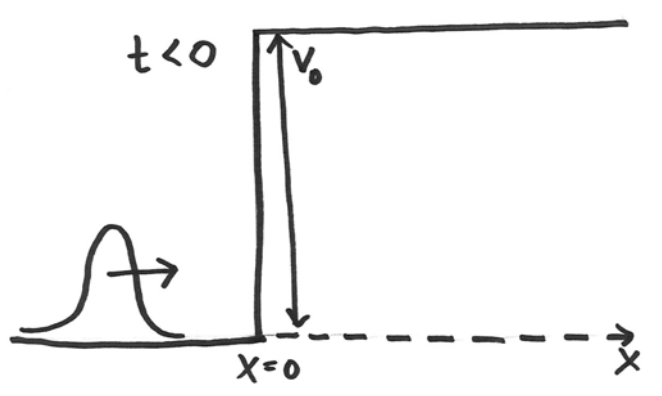
\includegraphics[width=0.4\linewidth]{resources/images/negative_t_step.png}
    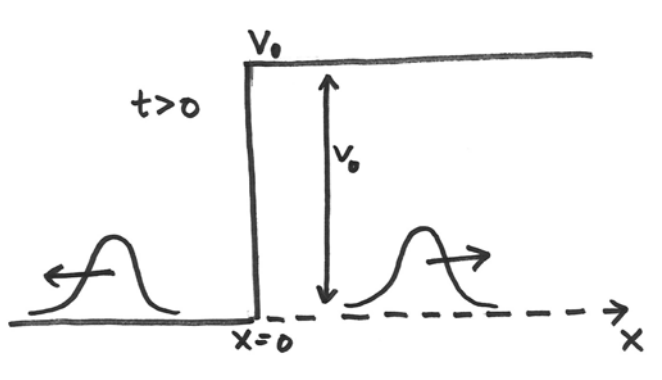
\includegraphics[width=0.45\linewidth]{resources/images/positive_t_step.png}
    \caption{A sketch of the behavior of the wavefunction for negative $t$ (left) and positive $t$ (right). Notice the incident, reflected, and transmitted wavepackets.}
    \label{step_potential_solution_sketch}
\end{figure}

\subsection{Wavepackets with Energy Below the Barrier}\label{wavepackets_energy_below_barrier}

We now consider a wavepacket built from eigenstates with energies $E<V_0$. Recall that in this situation $B/A=B=-e^{2i\delta(E)}$. Therefore, we have \begin{align*}\Psi_{inc}(x<0,t)&=\int_0^{\hat{k}} dk\,f(k)e^{ikx}e^{-iE(k)t/\hbar}, \\ \Psi_{ref}(x<0,t)&=-\int_0^{\hat{k}}dk\,f(k)e^{-ikx}e^{2i\delta(E)}e^{-iE(k)t/\hbar}.\end{align*}Note that the transmitted wave simply decays exponentially. However, the reflected wave is quite interesting. Using Theorem \ref{principle_stationary_phase} again, we have $$\frac{d}{dk}(2\delta(E)-kx-\frac{Et}{\hbar})\bigg|_{k_0}=0\implies2\delta'(E(k_0))\frac{\hbar^2k_0}{m}-x-\frac{\hbar k_0 t}{m}=0.$$Rearranging, we see that $$x=-\frac{\hbar k_0}{m}(t-2\hbar\delta'(E(k_0))).$$This represents a peak moving with constant negative velocity $-\frac{\hbar k_0}{m}<0$. However, there is also a \textbf{time delay} $\Delta t=2\hbar\delta'(E(k_0))$. Since the reflected wave is only defined for $x<0$, the peak does not begin to move until $t>2\hbar\delta'(E(k_0))$. We plotted $\delta(E)$ in Figure \ref{delta_step} and saw that its derivative diverges as $E$ approaches $0$ or $V_0$. Thus, the time delay is largest for wavepackets with very little energy or those with energy close to $V_0$.

\begin{framedrmk*}[Scattering theory]
    In scattering theory, physicists use this property of time delay to learn about unknown potentials by measuring the amount of time it takes for the reflected wave to begin moving. We will explore scattering theory in the next chapter.
\end{framedrmk*}

\section{Waves on the Finite Square Well}

\subsection{Reflection and Transmission Coefficients}\label{reflection_transmission_coefficients}

In Section \ref{finite_square_well}, we found the bound states of the finite square well potential $$V(x)=\begin{cases}0 & |x|>a \\ -V_0 & |x|<a\end{cases}$$

We now consider a scattering eigenstate with $E>0$ that represents an incoming wavefunction $Ae^{ikx}$ approaching the well from the left. Then the eigenstate will be of the form $$\psi(x)=\begin{cases}Ae^{ikx}+Be^{-ikx} & x<-a \\ Ce^{ik_2x}+De^{-ik_2x} & |x|<a \\ Fe^{ikx} & x>a\end{cases}$$The individual waves are depicted in Figure \ref{finite_square_well_scattering}.

\begin{figure}
    \centering
    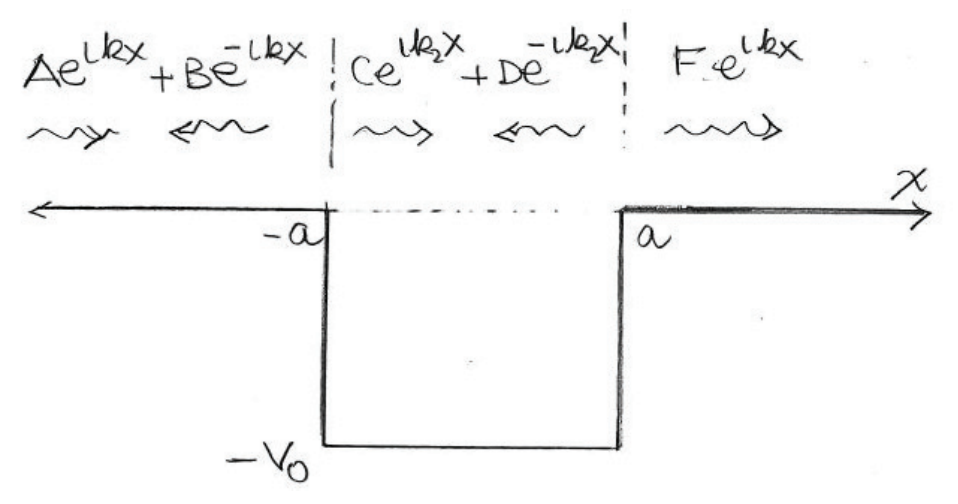
\includegraphics[width=0.5\linewidth]{resources/images/finite_square_well_scattering.png}
    \caption{Waves inside a finite square well.}
    \label{finite_square_well_scattering}
\end{figure}

Here $A$ is the coefficient of the incoming wave and $B$ is the coefficient of the reflected wave. Both of these waves have wavenumber $k$. In the well, there is a well moving to the right with coefficient $C$ and a wave moving to the left with coefficient $D$; both of these waves have wavenumber $k_2$. To the right of the well we have just one wave with coefficient $F$ moving to the right with wavenumber $k$. 

\begin{framedrmk*}[Symmetry breaking]
    Note that even though the potential is even, Corollary \ref{even_potential_cor} applies only to \textit{bound} states. Notably, the scattering states do not have to be even or odd. The symmetry is broken by the condition that the wave is incident from the left.
\end{framedrmk*}

\begin{framedrmk*}[Reflecting on a potential dip]
    In quantum mechanics, \textit{any} change in the potential can cause a reflection. This is the cause of the $B$ wave in Figure \ref{finite_square_well_scattering}; the incoming wave reflects off the potential dip at $x=-a$. This is similar to a string wave that encounters a change in the density of the string --- in general, there will always be a reflected and a transmitted component.
\end{framedrmk*}

The values of $k$ and $k_2$ are determined by the Schrödinger equation: $$k^2=\frac{2mE}{\hbar^2},\quad k_2^2=\frac{2m(E+V_0)}{\hbar^2}.$$There are four boundary conditions, given by continuity of $\psi$ and $\psi'$ at $x=-a$ and $x=a$. These four equations can be used to fix the coefficients $B$, $C$, $D$, and $F$ in terms of $A$. Since the outgoing waves to the left and right have the same wavenumber as the incoming wave, we define reflection and transmission coefficients $R$ and $T$ as $$R=\frac{|B|^2}{|A|^2},\quad T=\frac{|F|^2}{|A|^2}.$$From Theorem \ref{current_conservation_thm}, we know that the probability currents to the left and right of the well must be equal: $$|A|^2-|B|^2=|F|^2.$$Rearranging, $$\frac{|B|^2}{|A|^2}+\frac{|F|^2}{|A|^2}=R+T=1.$$

\subsection{Resonant Transmission}\label{resonant_transmission}

Solving for $R$ and $T$ is straightforward but a little tedious, so we will just quote the answer. The transmission coefficient is given by the following relation: $$\frac{1}{T}=1+\frac{1}{4}\frac{V_0^2}{E(E+V_0)}\sin^2(2k_2a).$$Since the second term is always positive, we have $T\leq 1$. As $E\to 0$, we have $\frac{1}{T}\to\infty$, so $T\to 0$. Also, as $E\to\infty$, we have $T\to 0$. Additionally, there is the possibility that $T=1$ if $\sin(2k_2a)=0$. This is called \textbf{resonant transmission}.

We can remove all units from this result by defining $$e=\frac{E}{V_0},\quad z_0^2=\frac{2ma^2V_0}{\hbar^2}.$$Then $$(k_2a)^2=\frac{2ma^2(E+V_0)}{\hbar^2}=\frac{2ma^2V_0}{\hbar^2}(1+e),$$so $$2k_2a=2z_0\sqrt{1+e}.$$We can similarly rewrite the $\frac{V_0^2}{E(E+V_0)}$ factor in terms of $e$. We get $$\boxed{\frac{1}{T}=1+\frac{1}{4e(1+e)}\sin^2(2z_0\sqrt{1+e}).}$$We now see that $T=1$ if $$2z_0\sqrt{1+e}=n\pi,\quad n\in\mathbb{Z}.$$Not all integers are allowed! Note that $e>0$ since the energy is positive. Thus, the left-hand side is at least $2z_0$, so $$n\geq \frac{2z_0}{\pi}.$$Let the associated energies be $E_n=e_nV_0$. Then $$e_n+1=\frac{n^2\pi^2}{4z_0^2}=\frac{n^2\pi^2\hbar^2}{2m(2a)^2V_0}.$$Multiplying both sides by $V_0$, we have $$E_n+V_0=\frac{n^2\pi^2\hbar^2}{2m(2a)^2}.$$Note that $E_n+V_0$ is the energy of the scattering state measured from the bottom of the finite square well. The right-hand side is the energy of the $n$th bound state of the \textit{infinite} square well of width $2a$, as shown in Figure \ref{resonant_transmission_well}. We thus have the following (rather surprising) result.

\begin{framedthm}[Resonant transmission in the finite square well]
    Resonant transmission in a finite square well occurs for those energies $E_n>0$ that are in the spectrum of the infinite square with the same width as our finite square well.
\end{framedthm}

\begin{figure}
    \centering
    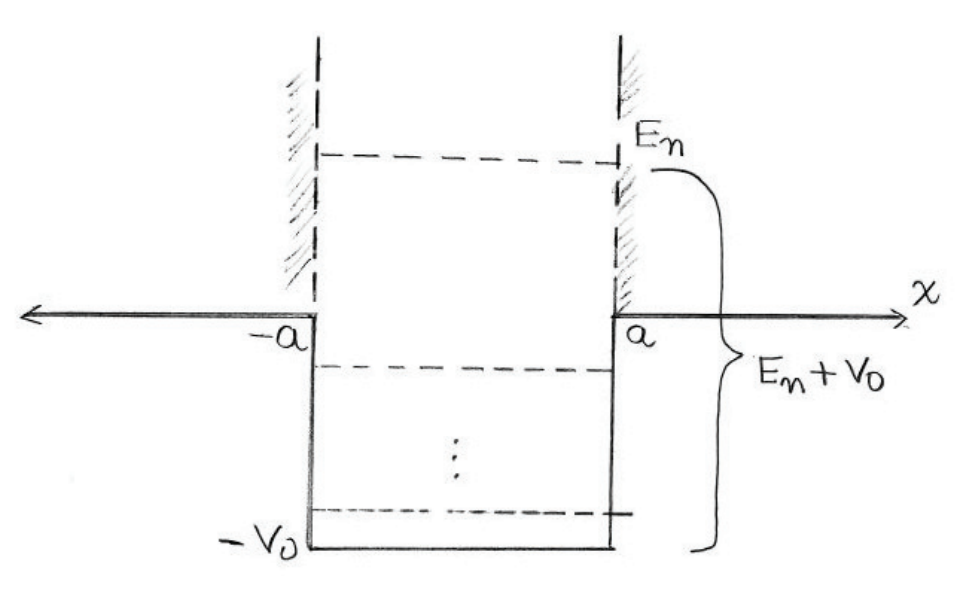
\includegraphics[width=0.5\linewidth]{resources/images/resonant_transmission_well.png}
    \caption{The energy levels for which resonant transmission occurs in the finite square well are precisely the energy levels of an equally-wide infinite square well.}
    \label{resonant_transmission_well}
\end{figure}

Since infinite square well bound states are characterized by fitting an integer number of half wavelengths inside the well, we have resonant transmission when the scattering waves fit perfectly inside the finite square well. This can also be seen directly from the vanishing of $\sin (k_2(2a))$ in the expression for $\frac{1}{T}$.

\begin{framedexpl}[Transmission coefficient for a given well]
    Figure \ref{resonant_transmission_example} depicts the transmission coefficient as a function of $e=E/V_0$ for a finite square well with $z_0=13\pi/4$. In this case, we must have $n\geq 7$. Notice that $T$ broadly approaches $1$ but only ever reaches it for discrete energy values.
\end{framedexpl}

\begin{figure}
    \centering
    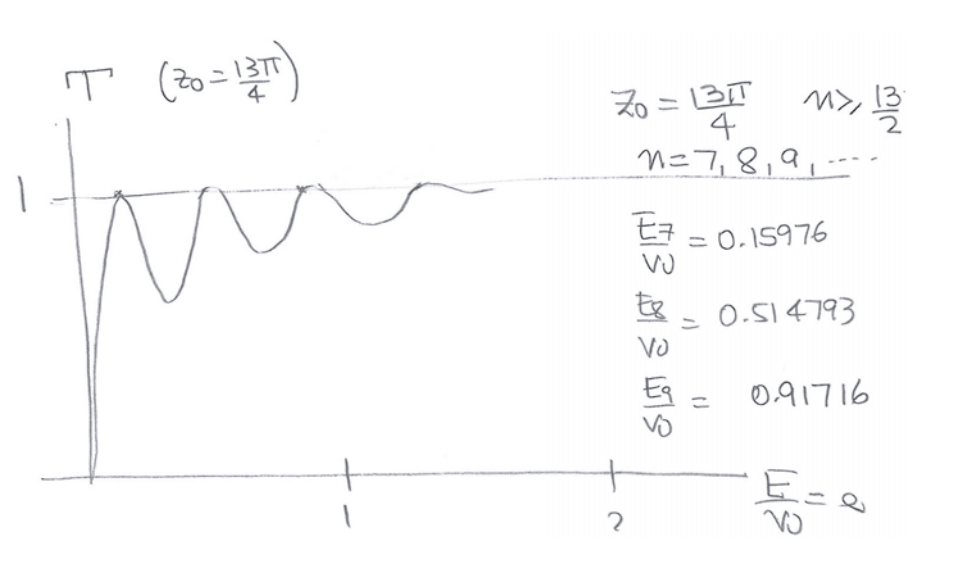
\includegraphics[width=0.65\linewidth]{resources/images/resonant_transmission_example.png}
    \caption{A graph of the transmission coefficient as a function of energy in a finite square well.}
    \label{resonant_transmission_example}
\end{figure}

\subsection{The Ramsauer-Townsend Effect}\label{ramsauer_townsend}

In 1921, Carl Ramsauer and John Sealy Townsend were studying the elastic scattering of low-energy electrons off of noble gas atoms. These gases have their electron shells fully filled and are both very un-reactive and have high ionization energies. 

Since the atom is electrically neutral, there is no potential far away from the atom. However, as the incident electron passes through the outer electron shell the potential due to this shell becomes $0$ by the Shell Theorem. The incident electron then experiences a spherically-symmetric attractive potential due to the nucleus-- some kind of finite spherical well. In the experiment, some electrons collided with the nuclei of the atoms and scattered, most bouncing back. Thus, we can view the reflection coefficient $R$ as a proxy for the scattering cross-section. 

Ramsauer and Townsend reported a very strange phenomenon. At very low energies, the scattering cross section was high. But as the energy was increased, the scattering went to $0$, and for it to go up again, the energy had to increase further. This behavior had no sensible classical explanation. 

In fact, this was an early example of quantum-mechanical resonant transmission. The reflection coefficient approaching $0$ meant the transmission coefficient going to $1$, which we know occurs for discrete values of $E$. Figure \ref{reflection_transmission_coefficients} displays both $R$ and $T$ as a function of energy. At the arrow, we have $R=0$, so there is no scattering. All of the electrons go straight through the atoms!

\begin{figure}
    \centering
    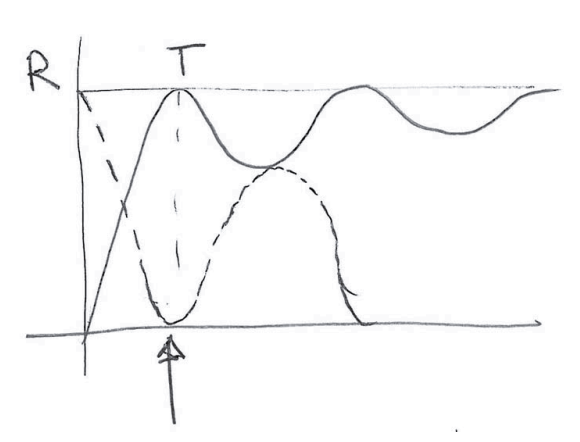
\includegraphics[width=0.5\linewidth]{resources/images/reflection_transmission_coeffs.png}
    \caption{A graph of the reflection coefficient $R$ and the transmission coefficient $T$ with respect to energy.}
  \label{reflection_transmission_coeffs}
\end{figure}
    
    \chapter{Scattering Theory}
    \section{Phase Shift}
\subsection{Finite Range Potentials}\label{finite_range_potentials}

Physicists learn a lot from scattering experiments. In fact, Rutherford first learned about the structure of the atom by scattering alpha particles (helium nuclei) off thin layers of gold. We have \textbf{elastic scattering} if particles do not change type; this typically exists for low energies. At high energies, scattering becomes quite complicated due to the creation of new particles.

The scattering of a particle off a fixed target is studied by working with a particle moving in a potential $V(x)$ created by the target. Even in the case of collisions, it is generally possible to study the problem using center of mass coordinates and considering scattering in a potential.

We consider elastic scattering in the general potential in Figure \ref{general_potential}.

\begin{figure}
    \centering
    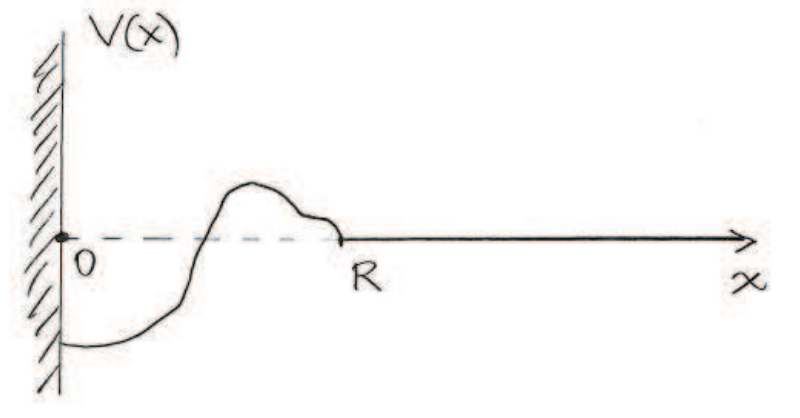
\includegraphics[width=0.5\linewidth]{resources/images/general_potential.png}
    \caption{A general potential $V(x)$.}
    \label{general_potential}
\end{figure}

This potential is given by $$V(x)=\begin{cases}\infty & x<0 \\V'(x) & 0<x<R \\ 0 & x>R\end{cases}$$We call this a \textbf{finite range potential}, because the nontrivial part of the potential $V'(x)$ exists only for a finite range $R$ from the origin. Furthermore, everything happens in $x>0$ because of an infinite wall at $x=0$. We imagine sending in incident waves from the right and analyzing the reflected waves. 

Consider first the case where $V'(x)=0$, so that $$V(x)=\begin{cases} 0 & x>0 \\ \infty & x\leq 0 \end{cases}$$ We have a free particle constrained to the positive real line. The solutions can be constructed using a linear combination of momentum eigenstates $e^{\pm ikx}$ where $$k^2=\frac{2mE}{\hbar^2}.$$Even better, we can divide this solution by $2i$ to find $$\boxed{\phi(x)=-\frac{e^{-ikx}}{2i}+\frac{e^{ikx}}{2i}=\sin kx.}$$The incoming wave is $-\frac{e^{-ikx}}{2i}$ and the reflected wave is $\frac{e^{ikx}}{2i}$. Both carry the same amount of probability current, so current conservation is satisfied. 

We now consider the more interesting case when $V'(x)\neq 0$. This potential still acts over a finite range $0<x<R$, and we will eventually be interested in computing the energy eigenstate wavefunction $\psi(x)$ in this region. However, we can first consider $\psi(x)$ *outside* the range of the potential. We will take the incoming wave to be the same as before: $$\text{Incoming wave:}\quad -\frac{e^{-ikx}}{2i}.$$The outgoing wave must have the same energy as the incident wave, so it must also have an $e^{ikx}$ factor: $$\psi(x)=-\frac{e^{-ikx}}{2i}+A\frac{e^{ikx}}{2i}.$$Note that $A$ cannot depend on $x$, since that would change the momentum of the outgoing wave. Furthermore, we found in Section \ref{energy_above_barrier} that the probability current of $Ae^{-ikx}+Be^{ikx}$ is proportional to $|A|^2-|B|^2$, so the only constant that we can attach to the outgoing wave is a pure phase $$A=e^{2i\delta(k)}.$$A natural range of $\delta$ would be from $0$ to $2\pi$, but it will turn out to be easier to let it range through all of $\mathbb{R}$ in order to get a \textit{continuous} function of $k$. 

Adding the incident and reflected waves, we get $$\psi(x)=\frac{1}{2i}(-e^{-ikx}+e^{ikx+2i\delta})=e^{i\delta}\frac{1}{2i}(-e^{-ikx-i\delta}+e^{ikx+i\delta}).$$Notably, this is equivalent to $$\boxed{\psi(x)=e^{i\delta}\sin (kx+\delta),\quad x>R.}$$

\subsection{Scattered Waves}\label{scattered_waves}

We consider the probability amplitudes of the solutions in the cases when $V'(x)=0$ and when $V'(x)\neq 0$. We have \begin{align*}|\phi(x)|^2&=\sin^2(kx),\\|\psi(x)|^2&=\sin^2(kx+\delta)\end{align*}Notice, therefore, that for any feature of $\phi(x)$ that we might find at some position $x_0$, we will find the same feature in $\psi(x)$ at $x=x_0-\frac{\delta}{k}$. This is depicted in Figure \ref{phase_shift_scattered_wave}. For $\delta>0$, the wave is ``pulled in'' by an amount $\delta/k$, and the potential is attractive. For $\delta<0$, the wave is ``pushed out'' by the same amount, and the potential is repulsive.

\begin{figure}
    \centering
    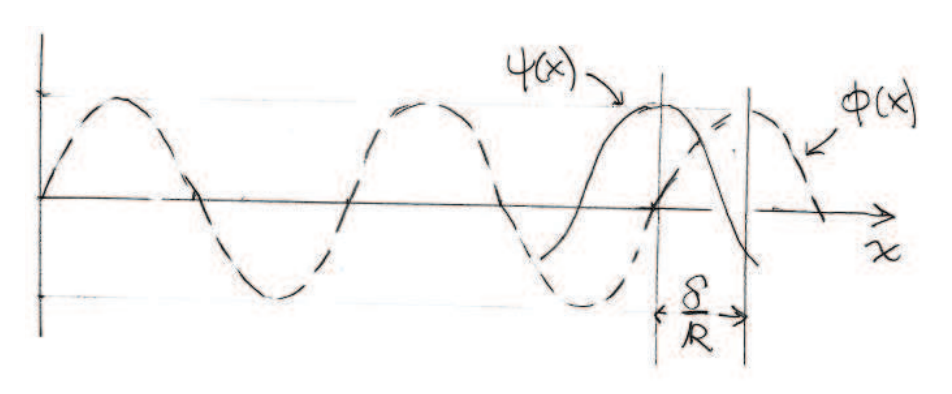
\includegraphics[width=0.5\linewidth]{resources/images/phase_shift_scattered_wave.png}
    \caption{The wave in the case of a nonzero potential is shifted by a distance $\frac{\delta}{k}$.}
    \label{phase_shift_scattered_wave}
\end{figure}

We define the \textbf{scattered wave} $\psi_s(x)$ as the extra wave in the solution $\psi(x)$ that would vanish for the case of zero potential. That is, we define $\psi_s(x)$ such that $$\psi(x)=\phi(x)+\psi_s(x).$$Recall that $\phi$ and $\psi$ have the same incident wave, so $\psi_s$ must be an outgoing wave. Indeed, we find $$\psi_s(x)=\psi(x)-\phi(x)=\frac{1}{2i}(-e^{-ikx}+e^{ikx+2i\delta}+e^{-ikx}-e^{ikx})=\frac{1}{2i}(e^{ikx+2\delta}-e^{ikx}).$$Factoring, we get $$\psi_s(x)=e^{i\delta}e^{ikx}\frac{1}{2i}(e^{i\delta}-e^{-i\delta})=e^{i\delta}\sin(\delta)e^{ikx}=A_se^{ikx},$$with $A_s=e^{i\delta}\sin\delta$. We call $A_s$ the \textbf{scattering amplitude}, since it is the amplitude of the scattered wave $\psi_s$. While these states cannot be normalized, the probability to scatter will be given by $$|A_s|^2=\sin^2\delta.$$

\subsection{Time Delay}\label{time_delay}

Consider an incident wavepacket given for $x>R$ by $$\psi_{inc}(x>R,t)=\int_0^\infty dk\,f(k)e^{-ikx}e^{-iE(k)t/\hbar},$$where $f(k)$ is a real function peaked around $k=k_0$. We find the reflected wavepacket by noting that $\psi_{inc}$ is a superposition of incident waves, so the reflection must be the associated superposition of reflected waves. We see that $$\psi_{ref}(x>R,t)=-\int_0^\infty dk\,f(k)e^{ikx}e^{2i\delta(k)}e^{-iE(k)t/\hbar}.$$We now use the stationary phase approximation to find the motion of the peak of the wavepacket. Recall that we must have a stationary phase when $k=k_0$. For the incident wave, we get that $$x=-\frac{\hbar k_0}{m}t=-v_gt,$$where $v_g$ is the group velocity. This makes sense; the peak of the incident wavepacket simply moves to the left with constant velocity. 

On the other hand, for the reflected wave, we get $$x=v_g\bigg(t-2\hbar\delta'(E(k_0))\bigg).$$Here we see the time delay $\Delta t=2\hbar\delta'(E)$, as stated in Section \ref{wavepackets_energy_below_barrier}. We can compare this delay to a natural time in the problem. We first write $$\Delta t=2\hbar\frac{dk}{dE}\frac{d\delta}{dk}=\frac{2}{(\frac{1}{\hbar}\frac{dE}{dk})}\frac{d\delta}{dk}=\frac{2}{(\frac{d\omega}{dk})}\frac{d\delta}{dk}=\frac{2}{v_g}\frac{d\delta}{dk}.$$Multiplying by $\frac{1}{R}$, we get that $$\frac{1}{R}\frac{d\delta}{dk}=\frac{\Delta t}{(\frac{2R}{v_g})}=\frac{\text{delay}}{\text{free transit time}}.$$Note that the right-hand side is the ratio of the time delay to the time it would take a free particle to travel in and out of the range of the potential.

\begin{framedexpl}[Phase shift for a potential well]
    Find the energy eigenstates of the potential in Figure \ref{phase_shift_potential_well} given by $$V(x)=\begin{cases} -V_0 & 0<x<a \\ 0 & x>a \\ \infty & x<0 \end{cases}$$
\end{framedexpl}

\begin{figure}[H]
    \centering
    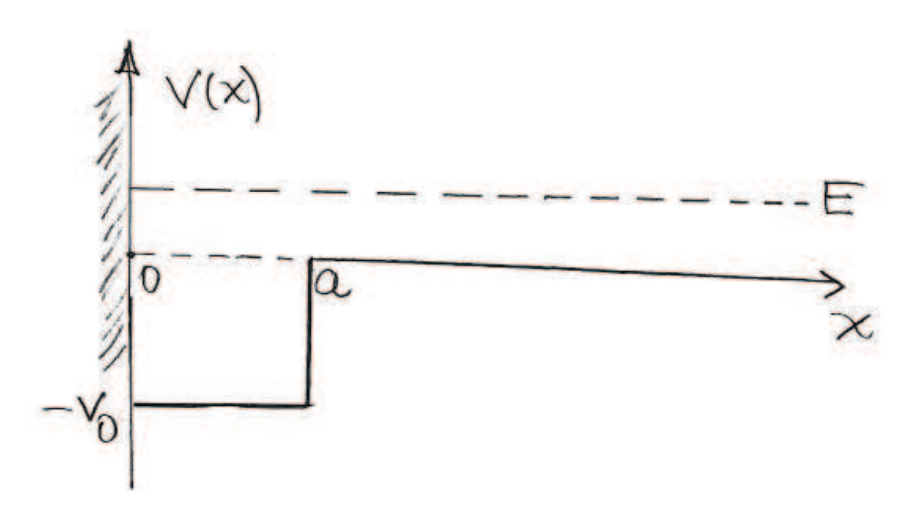
\includegraphics[width=0.5\linewidth]{resources/images/phase_shift_potential_well.png}
    \caption{A potential well with width $a$ and depth $V_0$.}
    \label{phase_shift_potential_well}
\end{figure}

\begin{framedansw}
    We found in Section \ref{finite_range_potentials} that the solution outside the well is of the form $e^{i\delta}\sin(kx+\delta)$. Inside the well, the boundary condition $\psi(0)=0$ forces the solution to be a sine, giving us $$\psi(x)=\begin{cases}e^{i\delta}\sin(kx+\delta) & x>a \\ A\sin(k'x) & 0<x<a\end{cases}$$where $$k^2=\frac{2mE}{\hbar^2},\quad k'^2=\frac{2m(E+V_0)}{\hbar^2}.$$The boundary conditions at $x=a$ give \begin{align*}A\sin(k'a)&=e^{i\delta}\sin(ka+\delta), \\ k'A\cos(k'a) &= ke^{i\delta}\cos(ka+\delta).\end{align*}Dividing the second equation by the first, we have $$k\cot(ka+\delta)=k'\cot(k'a).$$We now use the identity $$\cot(A+B)=\frac{\cot A\cot B-1}{\cot A+\cot B},$$which gives us $$\frac{k'}{k}\cot(k'a)=\cot(ka+\delta)=\frac{\cot(ka)\cot(\delta)-1}{\cot(ka)+\cot(\delta)}.$$Solving this equation for $\delta$ yields $$\boxed{\cot\delta=\frac{\tan(ka)+\frac{k'}{k}\cot(k'a)}{1-\frac{k'}{k}\cot(k'a)\tan(ka)}}.$$
    As usual, we characterize the well by the unit-free constant $$z_0=\frac{2mV_0a^2}{\hbar^2}.$$We also have$$(k'a)^2=z_0^2+(ka)^2.$$Using this relation, and letting $ka=u$, we can solve for $\delta$ solely in terms of the unit-free constants $u$ and $z_0$: $$\tan\delta=\frac{1-\sqrt{1+(z_0/u)^2}\cot(\sqrt{z_0^2+u^2})\tan u}{\tan u+\sqrt{1+(z_0/u)^2}\cot(\sqrt{z_0^2+u^2})}.$$

\end{framedansw}

\begin{framedrmk*}[Messy formulas]
    When dealing with phase shifts, many of the resulting formulas will seem forbiddingly complicated, even when simplified as far as possible. Remember that it is always possible to plot such a formula with a computer for various values of $V_0$.
\end{framedrmk*}

\subsection{Excursion of the Phase Shift}

Figure \ref{phase_shift_plots} shows the phase shift $\delta$, the scattering probability $\sin^2\delta$, the time delay $\frac{1}{a}\frac{d\delta}{dk}$, and the wavefunction amplitude $A$ inside the well as functions of $u=ka$, a unit-free proxy for the energy, for $z_0=0.59\pi$.

\begin{figure}
    \centering
    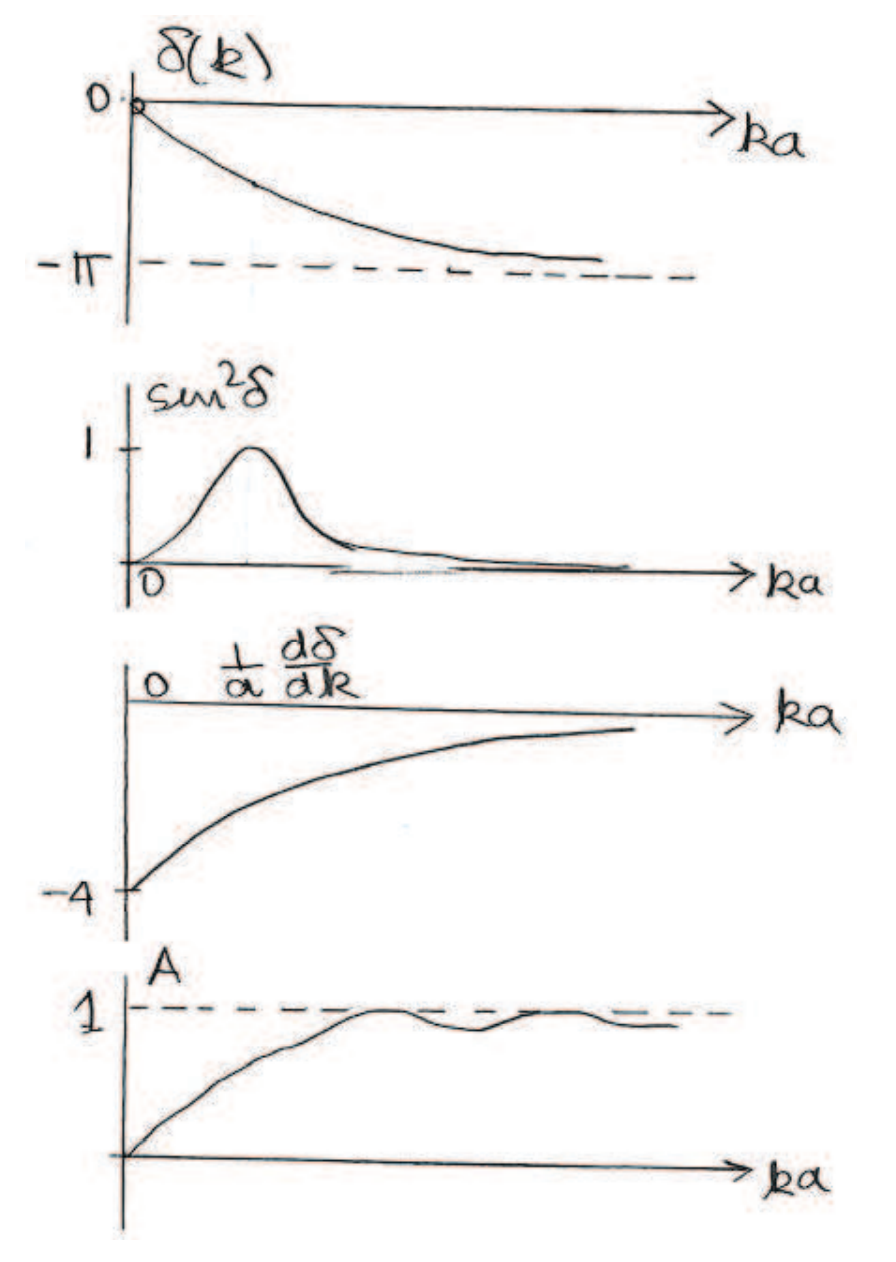
\includegraphics[width=0.45\linewidth]{resources/images/phase_shift_plots.png}
    \caption{Four plots for the potential well with $z_0=0.59\pi$.}
    \label{phase_shift_plots}
\end{figure}

Note that the phase $\delta$ begins at $0$ for $0$ energy and approaches $-\pi$ for infinite energy. The \textbf{phase excursion} is thus $\pi$. In the next section, we will prove a relationship between the phase excursion and the number of bound states of the potential. Since $z_0$ is in the range $(\frac{\pi}{2},\pi)$, the half-square well with this value of $z_0$ has one bound state.

The value of $|A_s|^2=\sin^2\delta$ represents the probability of scattering and peaks for the value of $ka$ for which $|\delta|=\pi/2$.

Next we have the unit-free time delay $\frac{1}{a}\frac{d\delta}{dk}$. Note that the delay is always negative. This is because as the particle moves over the well, its kinetic energy increases by $V_0$, so it speeds up.

Finally, the last plot shows the magnitude $A$ of the constant that gives the amplitude of the wavefunction within the well. This is identical to Figure \ref{resonant_transmission_example}.

At very large energy, the particle barely notices the potential; the phase shift approaches $-\pi$, which is equivalent to approaching $0$ and having no phase shift. Accordingly, $|A_s|^2$ approaches $0$, so no scattering occurs, and the time delay also approaches $0$. Finally, $A\to 1$, so the amplitude of the wavefunction is unaffected by the well.

\subsection{Levinson's Theorem}

We now reach one of the most challenging and counterintuitive results in this course. \textbf{Levinson's theorem} relates the number of bound states of a potential to the excursion of the phase shift as energy ranges from $0$ to $\infty$.

\begin{framedthm}[Levinson's theorem]
    The number $N_b$ of bound states of a potential is related to the excursion of the phase shift $\delta(E)$ by the relation $$\boxed{N_b=\frac{1}{\pi}\bigg(\delta(0)-\delta(\infty)\bigg).}$$
\end{framedthm}

\begin{proof}
    Consider an arbitrary potential $V(x)$ of range $R$, with an infinite wall at $x=0$ (shown to the left in Figure \ref{regulator}). This potential has a finite number of bound states. However, the scattering states belong to a continuum and are uncountable. To be able to count all the states, we place another infinite wall at $x=L$, thus discretizing the scattering states and making them countable. We call this second wall the \textbf{regulator}, and the new potential (shown to the right) the \textbf{regulated potential}. Of course, the spectrum will be different for the regulated potential, but these changes become negligible as $L$ goes to infinity.

    The key of the proof will be to compare counting the states in the regulated potential to those in the $V=0$ potential, also regulated with a wall at $x=L$. Consider the positive energy eigenstates of the regulated $V=0$ potential. These correspond to the wavefunctions $\phi(x)=\sin kx$, with the second wall requiring $\phi(L)=0$. We thus have $$kL=n\pi,\quad n\in\mathbb{N}.$$The values of $k$ have been quantized. Let $dk$ be an infinitesimal interval in wavenumber with $dn$ the number of states within in the interval when $V=0$. We have $$dn=\frac{L}{\pi}dk.$$
    
    Recall that when $V(x)$ is an arbitrary finite-range potential, the solutions for $x>R$ -- all of which are positive-energy solutions -- have the form $$\psi(x)=e^{i\delta}\sin(kx+\delta).$$The boundary condition $\psi(L)=0$ due to the regulator implies the quantization $$kL+\delta(k)=n'\pi,\quad n'\in\mathbb{Z}.$$We again differentiate to determine the number of positive-energy states $dn'$ within the infinitesimal interval $dk$ in wavenumber: $$dn'=\frac{L}{k}dk+\frac{1}{\pi}(\frac{d\delta}{dk})dk.$$Imagine slowly deforming the initial $V=0$ potential to get to the potential $V$. Notice that in this process, we lose some number of positive-energy solutions in the interval $dk$, given by $$dn-dn'=-\frac{1}{\pi}(\frac{d\delta}{dk}dk).$$The total number of positive energy solutions lost as the potential $V$ is turned on given by integrating the above result over the full range of $k$: $$\text{lost positive-energy solutions}=-\int_0^\infty\frac{1}{\pi}\frac{d\delta}{dk}dk=-\frac{1}{\pi}(\delta(\infty)-\delta(0)).$$However, in the process of slowly deforming the potential, states do not disappear. Therefore, the lost positive-energy states must now appear as \textit{negative-energy states}, or bound states! This process is depicted in Figure \ref{levinson_diagram}. Letting $N_b$ denote the number of bound states in the new potential $V$, we arrive at our intended result $$N_b=\frac{1}{\pi}(\delta(0)-\delta(\infty)).$$
\end{proof}

\begin{figure}
    \centering
    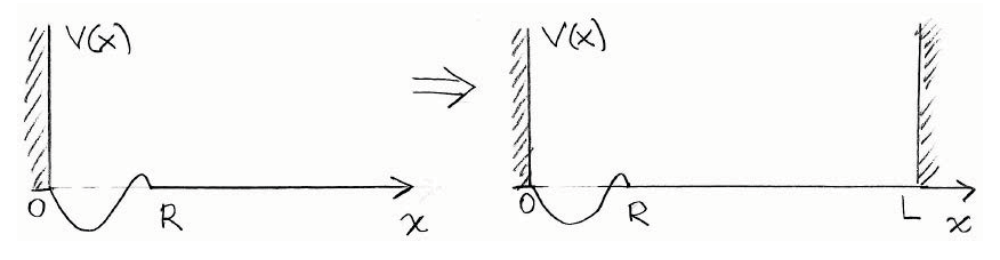
\includegraphics[width=0.5\linewidth]{resources/images/regulator.png}
    \caption{An arbitrary potential $V(x)$ (left) and the regulated potential (right).}
    \label{regulator}
\end{figure}

\begin{figure}
    \centering
    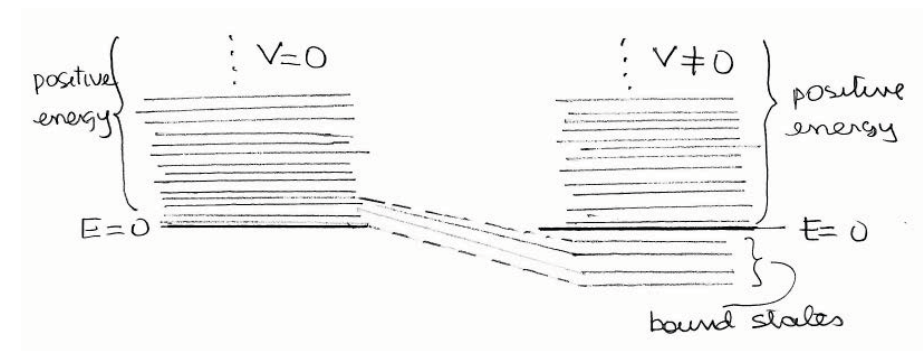
\includegraphics[width=0.5\linewidth]{resources/images/levinson_diagram.png}
    \caption{As $V$ is turned on, some positive-energy states are lost, instead becoming negative-energy bound states.}
    \label{levinson_diagram}
\end{figure}

\section{Resonance}
\subsection{Arbitrary Time Delay}

We have previously found the time delay $\Delta t=2\hbar\delta'(E)$ associated with the reflected wavepacket that emerges from a finite-range potential. If the time delay is negative, the reflected wave emerges ahead of time, and if the time delay is positive, the reflected wave emerges late. We introduce the subject of resonances by asking the following question.

\begin{framedquest*}
    Can we get an arbitrarily large negative time decay?
\end{framedquest*}

The answer is no. If the time delay was sufficiently large, it would violate causality: the incoming packet would be reflected even before it reached the potential, which is impossible. In fact, the largest possible negative time delay should be as if we had perfect reflection when the incoming packet hit $x=R$.\footnote{This argument seems solid, but there are actually some subtle quantum corrections for the largest possible negative time delay. Luckily, these vanish for packets with large energy, and our final constraint is quite accurate.} In this case, the time delay would be $-\frac{2R}{v_0}$, where the packet has velocity $v_0$. Thus, we expect $$\Delta t=2\hbar\frac{d\delta}{dE}\geq -\frac{2R}{v_0}.$$This can be simplified a bit: $$2\hbar\frac{1}{\frac{dE}{dk}}\frac{d\delta}{dk}=2\hbar\frac{1}{\hbar v_0}\frac{d\delta}{dk}\geq -\frac{2R}{v_0},$$which produces the constraint $$\frac{d\delta}{dk}\geq -R.$$  

We can also ask the opposite question.

\begin{framedquest*}
    Can we get an arbitrarily large positive time delay?
\end{framedquest*}

The answer is yes! This can happen if the wavepacket gets temporarily trapped in the potential, in which case we expect the probability amplitude to become extremely large in the $0<x<R$ region. If the wavepacket is trapped for a long time, we have a \textbf{resonance}. The state is a bit like a bound state in that it gets localized in the potential, at least for a while. We can achieve this with the potential $$V(x)=\begin{cases}\infty & x\leq 0 \\ -V_0 & 0<x<a \\ V_1 & a<x<2a \\ 0 & x>2a\end{cases}$$This potential is shown in Figure \ref{resonant_potential}. The particle gets trapped for a long time in the well from $x=0$ to $x=a$, but it has some small probability of leaking through the $V_1$ barrier. 

\begin{figure}
    \centering
    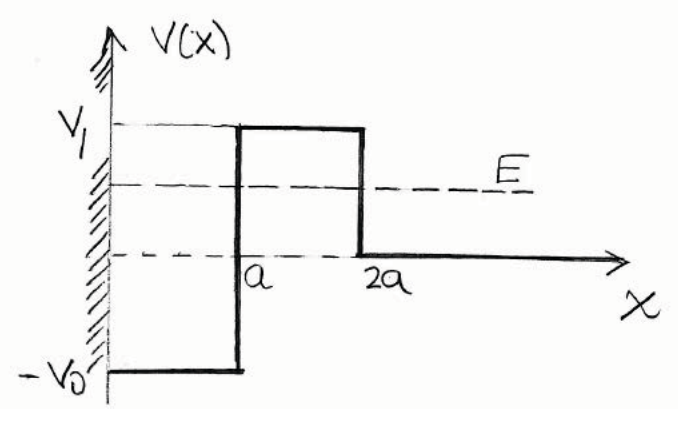
\includegraphics[width=0.5\linewidth]{resources/images/resonant_potential.png}
    \caption{A potential well with a barrier.}
    \label{resonant_potential}
\end{figure}

We search for resonances with energies in the range $0<E<V_1$; this is the range for which we may have an incoming wave in the $x>2a$ region but not in the $a<x<2a$ region. 

We define $$k^2=\frac{2mE}{\hbar^2},\quad k'^2=\frac{2m(E+V_0)}{\hbar^2},\quad \kappa^2=\frac{2m(V_1-E)}{\hbar^2}.$$In the region $0<x<a$ we use trigonometric functions of $k'x$. In the region $a<x<2a$ we use hyperbolic functions of $\kappa a$. Finally, in the region $x>2a$ we use the canonical solution $\psi(x)=e^{i\delta}\sin(kx+\delta)$.

Since $\psi(0)=0$, we must have a sine function in the first region. The solution in the second region can be written as a linear combination of $\cosh\kappa(x-a)$ and $\sinh\kappa(x-a)$, which we choose in order to force continuity at $x=a$: $$\psi(x)=\begin{cases}A\sin(k'x) & 0<x<a \\ A\sin(k'a)\cosh\kappa(x-a)+B\sinh\kappa(x-a) & a<x<2a\\ e^{i\delta}\sin(kx+\delta) & x>2a\end{cases}$$

After implementing the remaining boundary conditions, we can solve for the phase shift $\delta$. The final answer is $$\tan(2ka+\delta)=\frac{ka}{\kappa a}\frac{\sin(k'a)\cosh(\kappa a)+\frac{k'}{k}\cos(k'a)\sinh(\kappa a)}{\sin(k'a)\sinh(\kappa a)+\frac{k'}{\kappa}\cos(k'a)\cosh(\kappa a)}.$$

This expression is very complicated, so it's best to use a computer to do numerical work. For this we define $$z_0^2=\frac{2mV_0a^2}{\hbar^2},\quad z_1^2=\frac{2mV_1a^2}{\hbar^2},\quad u=ka.$$Then we can express both $k'a$ and $\kappa a$ as functions of these unit-free constants: $$(k'a)^2=z_0^2+u^2,\quad (\kappa a)^2=z_1^2-u^2.$$We also let $e=\frac{E}{V_1}$ be a unit-free proxy for the energy, so that $$e=\frac{E}{V_1}=\frac{\hbar^2k^2a^2}{2mV_1a^2}=\frac{u^2}{z_1^2}.$$

\subsection{Example of a Resonance}\label{resonance_example}

We are now ready to make some plots. In Figure \ref{resonance_plots}, we show results for $z_0^2=1$ and $z_1^2=5$ (since $e<1$, this constrains $u<\sqrt{5}$).

\begin{figure}
    \centering
    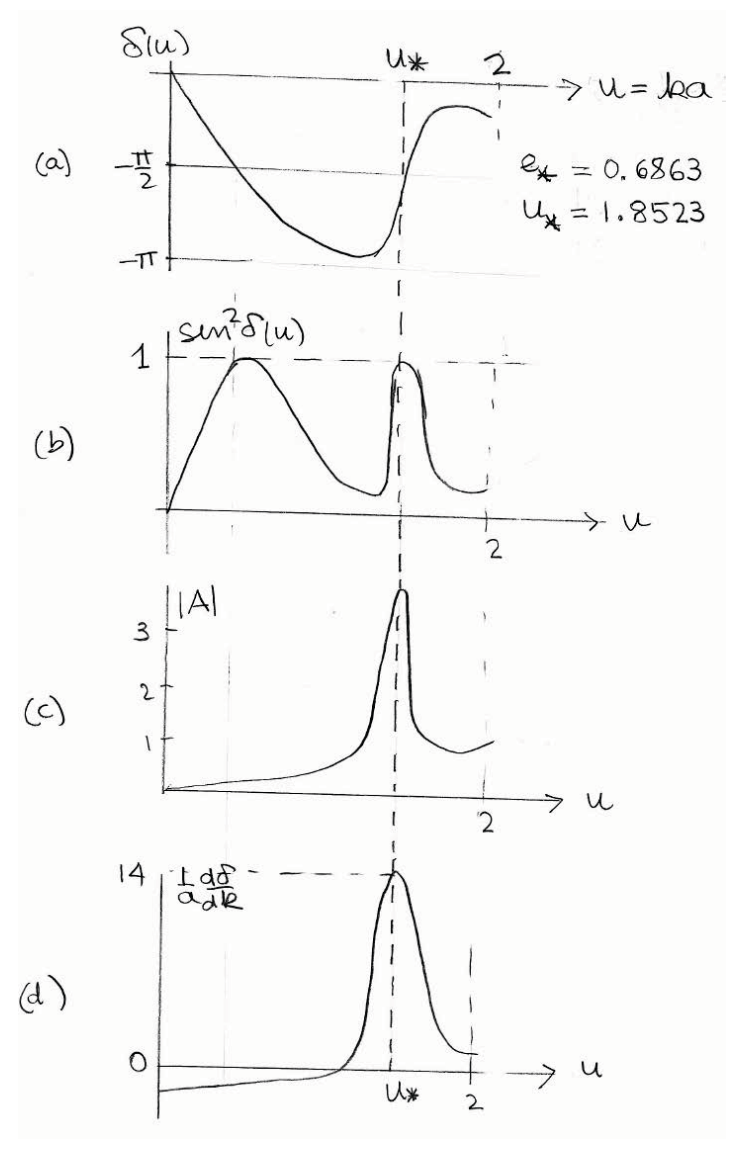
\includegraphics[width=0.4\linewidth]{resources/images/resonance_plots.png}
    \caption{Four plots for the potential with $z_0^2=1$ and $z_1^2=5$.}
    \label{resonance_plots}
\end{figure}

In part (a) of the figure, we see that $\delta(ka)$ begins by decreasing linearly, indicating a negative time delay. This is due to the low-energy waves reflecting at $x=2a$ off the $V_1$ barrier. However, as $u$ approaches $u_* \approx 1.8523$, $\delta$ increases rapidly from $\approx -\pi$ to $\approx 0$. In fact, we get a resonance at $u_*$, indicated by the peaks in the amplitude within the well in part (c) and the unit-free time delay in part (d). At $u_*$, this time delay reaches a value of about 14, meaning the delay is 14 times the free transit time $4a/v_0$!

\subsection{Modeling a Resonance}\label{modeling_a_resonance}

We've now seen an example of a resonance, but how do we find resonances formulaically? Suppose there exists a resonance at $k=\alpha$. We claim that this can be achieved by the function $$\tan\delta=\frac{\beta}{\alpha-k}.$$The plots of $\frac{\beta}{\alpha-k}$ and the arctangent of this quantity are shown in Figure \ref{resonance_modeling}. Note that the argument varies quickly in the region $(\alpha-\beta,\alpha+\beta)$. To have a resonance, we must have a sharp increase in $\delta$. Thus, the width of this region must be small, i.e. we must have $\beta\ll\alpha$.

\begin{figure}
    \centering
    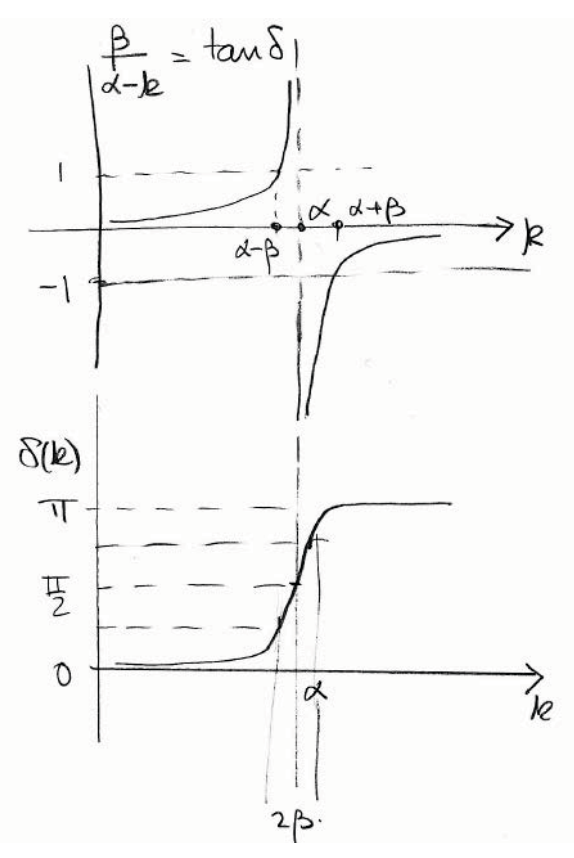
\includegraphics[width=0.4\linewidth]{resources/images/resonance_modeling.png}
    \caption{Plots of $\tan\delta$ and $\delta(k)$.}
    \label{resonance_modeling}
\end{figure}

We can also calculate $$\frac{d\delta}{dk}\bigg|_{k=\alpha}=\frac{1}{\beta},\quad|\psi_s|^2=\sin^2\delta=\frac{\beta^2}{\beta^2+(\alpha-k)^2}.$$The first result indicates that the time delay is inversely proportional to $\beta$ -- thus, resonance does indeed require small $\beta$, as reasoned above. The second gives the scattering amplitude as a function of $k$, with a peak at $k=\alpha$. This equation is most famously expressed in terms of *energy*, not momentum. Note that $$E-E_\alpha=\frac{\hbar^2}{2m}(k^2-\alpha^2)=\frac{\hbar^2}{2m}(k+\alpha)(k-\alpha).$$For $k\approx\alpha$, this is roughly equal to $\frac{\hbar^2}{2m}(2\alpha)(k-\alpha)$. It follows that $$(k-\alpha)^2\approx\frac{m^2}{\hbar^4\alpha^2}(E-E_\alpha)^2,$$and therefore $$|\psi_s|^2\approx\frac{\beta^2}{\beta^2+\frac{m^2}{\hbar^4\alpha^2}(E-E_\alpha)^2}=\frac{\frac{1}{4}\Gamma^2}{(E-E_\alpha)^2+\frac{1}{4}\Gamma^2},$$where $\Gamma$ is a constant with units of energy given by $$\Gamma=\frac{2\alpha\beta\hbar^2}{m}.$$The energy dependence of $|\psi_s|^2$ is called the \textbf{Breit-Wigner distribution}.

\begin{frameddefn}[Breit-Wigner Distribution]
    For resonance near $k=\alpha$, the probability amplitude of the scattered wave follows the distribution $$\boxed{|\psi_s|^2\approx\frac{\frac{1}{4}\Gamma^2}{(E-E_\alpha)^2+\frac{1}{4}\Gamma^2}.}$$
\end{frameddefn}

This distribution is shown in Figure \ref{breit_wigner_distribution}. The peak value $|\psi_s|^2=1$ is obtained for $E=E_\alpha$. We call $\Gamma$ the width at half maximum because the value of $|\psi_s|^2$ at $E=E_\alpha\pm\frac{1}{2}\Gamma$ is $\frac{1}{2}$. Small $\Gamma$ corresponds to a narrow width, or a narrow resonance.

\begin{figure}
    \centering
    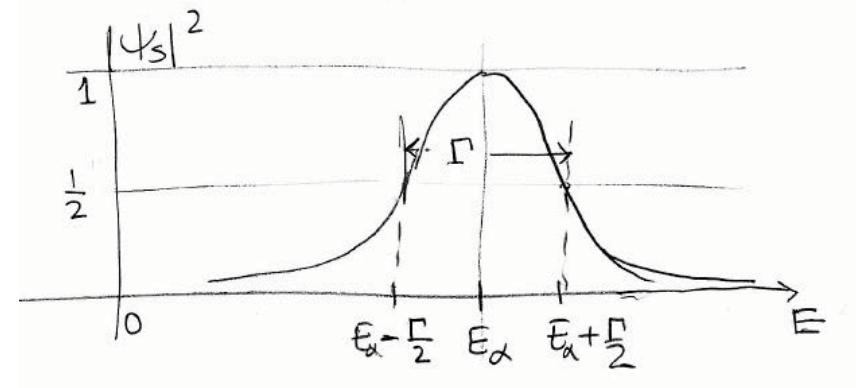
\includegraphics[width=0.5\linewidth]{resources/images/breit_wigner_distribution.png}
    \caption{A graph of the Breit-Wigner distribution. As shown, $\Gamma$ is the width at half maximum.}
    \label{breit_wigner_distribution}
\end{figure}

\subsection{Half-Width and Time Delay}\label{half_width_time_delay}

To better understand the significance of $\Gamma$, we define the associated time $\tau$, called the \textbf{lifetime} of the resonance: $$\tau=\frac{\hbar}{\Gamma}=\frac{m}{2\alpha\beta\hbar}.$$As you would expect, the lifetime is closely related to the time delay associated with a wavepacket at the resonant value $\alpha$ of $k$. We can evaluate this time delay: \begin{align*}\Delta t&=2\hbar\frac{d\delta}{dE}\\&=2\hbar\frac{dk}{dE}\frac{d\delta}{dk}\bigg|_{k=\alpha}\\&=\frac{2\hbar}{(\frac{\hbar^2k}{m})}(\frac{1}{\beta})\\&=\frac{2\hbar}{(\frac{\hbar^2\alpha\beta}{m})}\\&=\frac{2m}{\alpha\beta\hbar}=4\tau.\end{align*}Thus, the lifetime is simply one-fourth of the time delay.

\begin{framedrmk*}
    Unstable particles can be thought of as resonances. The Higgs boson, discovered in 2012, is an unstable particle with mass $E_\alpha=125$ GeV. It can decay into two photons, or into two taus, or into a $b\bar{b}$ pair, among others. The width $\Gamma$ associated with the Higgs is $4.07$ MeV $(\pm4\%)$. Its lifetime $\tau$ is about $1.62\times 10^{-22}$ seconds!
\end{framedrmk*}

\subsection{Resonances in the Complex $k$-Plane}\label{resonances_complex_plane}

We now try to understand resonances more mathematically. We saw that, at resonance, the norm of $A_s$ reaches a maximum value of $1$. Let's see what happens when $A_s$ is large. We have $$A_s=\sin\delta e^{i\delta}=\frac{\sin\delta}{e^{-i\delta}}=\frac{\sin\delta}{\cos\delta-i\sin\delta}=\frac{\tan\delta}{1-i\tan\delta}.$$At resonance, $\delta=\pi/2$ and $A_s=i$. On the other hand, if we \textit{really} want $A_s$ to be large, notice that $A_s$ becomes \textit{infinite} for $$\tan\delta=-i.$$This seems nonsensical! For the tangent of the phase shift to be complex, $\delta$  must also be complex, whatever that means. But let's think this through a bit more. Recall that near a resonance, $\tan\delta=\frac{\beta}{\alpha-k}.$ Then we have $$A_s=\frac{\frac{\beta}{\alpha-k}}{1-i\frac{\beta}{\alpha-k}}=\frac{\beta}{(\alpha-i\beta)-k}.$$At the resonant energy, $k=\alpha$, which gives $A_s=i$, as expected. If we instead think of the wavenumber $k$ as a \textit{complex} variable, we see that $A_s$ becomes infinite at $k=k_*=\alpha-i\beta$. (In complex analysis, this point is called a \textbf{pole}). This is the true location of the resonance! The real part is the resonant energy, and the imaginary part encodes the lifetime.

For small $\beta$, the resonance occurs near the real axis, as shown in Figure \ref{resonance_complex_plane}. As mentioned in Section \ref{modeling_a_resonance}, a smaller $\beta$ means a sharper resonance. As we can see, the value of $|A_s|$ on the real line becomes large for $k=\alpha$ because of its proximity to $k=k_*$. 

The lesson here is that we can search for resonances mathematically by solving for the complex $k$ values for which $$\boxed{\tan\delta(k)=-i.}$$The real parts of these $k$'s will be the resonant energies, and the imaginary parts will be the lifetimes.

The idea of a complex $k$ plane is very powerful. Suppose we consider purely imaginary values $k=i\kappa$, with $\kappa\in\mathbb{R}_+$. Then the energy takes the form $$E=-\frac{\hbar^2\kappa^2}{2m}<0,$$which can represent bound states. Indeed, one can plot the bound states in the complex $k$ plane along the positive imaginary axis, as shown in Figure \ref{resonance_complex_plane}. The complex $k$ plane has room to fit scattering states, resonances, and bound states!

\begin{figure}
    \centering
    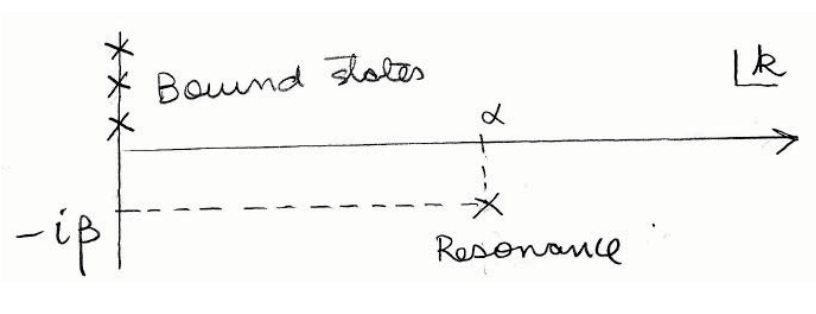
\includegraphics[width=0.5\linewidth]{resources/images/resonance_complex_plane.png}
    \caption{Resonances can be thought of as occurring for complex values of $k$, where the real part is the resonant energy and the imaginary part is the lifetime.}
    \label{resonance_complex_plane}
\end{figure}

\begin{framedrmk*}[Anti-bound states]
    Some physicists even include \textit{anti-bound states} on the \textit{negative} imaginary axis of the complex $k$ plane. While normal bound states are characterized by exponential decay in the classically forbidden region, anti-bound states are characterized by exponential \textit{increase} in this region. This may seem strange, but these states can actually be observed in nuclear physics, when a neutron is captured by some light nucleus.
\end{framedrmk*}


    \chapter{Central Potentials}
    \section{Angular Momentum Operators}
\subsection{Generators}\label{generators}

So far, we've considered several Hermitian operators: the position operator $\hat{x}$, the momentum operator $\hat{p}$, and the energy operator, or Hamiltonian, $\hat{H}$. As we begin our work in $3$ dimensions, we now discuss yet another operator: angular momentum. Like momentum, it is a vector operator. It will have three components, each of which is Hermitian and thus represents a measurable quantity. Although the definition of the angular momentum operator will be motivated by its classical counterpart, we will see unexpected quantum properties.

It turns out that the momentum operator has something to do with translations; specifically, consider the operator $$e^{\frac{i\hat{p}a}{\hbar}},$$where $a$ is a constant with units of length, acting on a wavefunction $\psi$: $$e^{\frac{i\hat{p}a}{\hbar}}\psi(x)=e^{a\frac{d}{dx}}\psi(x)=\sum_{n=0}^\infty\frac{1}{n!}\bigg(a\frac{d}{dx}\bigg)^n\psi(x).$$Expanding the sum gives $\psi(x)+a\frac{d\psi}{dx}+\frac{a^2}{2!}\frac{d^2\psi}{dx^2}+\frac{a^3}{3!}\frac{d^3\psi}{dx^3}+\ldots$ Note that this is simply the Taylor series expansion of $\psi(x+a)$. This means that the operator $e^{\frac{i\hat{p}a}{\hbar}}$ moves the wavefunction a displacement of $-a$. We say that the momentum operator \textbf{generates} translations. Similarly, we will show that the \textit{angular} momentum operator generates \textit{rotations}.

\begin{framedrmk*}[Types of angular momentum]
    There are two types of angular momentum: \textbf{orbital} and \textbf{spin}. Orbital angular momentum is the familiar kind that occurs when a particle rotates around some fixed point. But there is also spin angular momentum, which is carried by point particles that somehow possess angular momentum despite having no apparent size. Much of the mathematics of angular momentum is valid for both orbital and spin angular momentum.
\end{framedrmk*}

\subsection{Schrödinger Equation for a Central Potential}\label{schrodinger_central_potential}

Let's begin our analysis of angular momentum by recalling that in three dimensions the usual position and momentum operators are vector operators: \begin{align*}\hat{\mathbf{p}}&= (\hat{p}_x,\hat{p}_y,\hat{p}_z)=\frac{\hbar}{i}\nabla=\frac{\hbar}{i}\bigg(\frac{\partial}{\partial x},\frac{\partial}{\partial y},\frac{\partial}{\partial z}\bigg),\\\hat{\mathbf{x}}&=(\hat{x},\hat{y},\hat{z}).\end{align*}The commutation relations are $$[\hat{x},\hat{p}_x]= [\hat{y},\hat{p}_y]=[\hat{z},\hat{p}_z]=i\hbar.$$All other commutators involving the position and momentum operators are zero.

Consider a particle represented by a three-dimensional wavefunction $\psi(x,y,z)$ moving in a potential $V(\mathbf{r})$. The three-dimensional Schrödinger equation takes the form $$-\frac{\hbar^2}{2m}\nabla^2\psi(\mathbf{r})+V(\mathbf{r})\psi(\mathbf{r})=E\psi(\mathbf{r}).$$We have a \textbf{central potential} if $V$ is spherically symmetric -- that is, if $V(\mathbf{r})=V(r)$. Then the equipotential surfaces are spheres centered at the origin. For a central potential, the above equation is $$-\frac{\hbar^2}{2m}\nabla^2\psi(\mathbf{r})+V(r)\psi(\mathbf{r})=E\psi(\mathbf{r}).$$Note that the wavefunction is *not* necessarily spherically symmetric; in fact, it will only be for the simplest kinds of solutions. Given the rotational symmetry of the potential, however, we express the following equations in spherical coordinates. The Laplacian is given by $$\nabla^2\psi=(\nabla\cdot\nabla)\psi=\frac{1}{r}\frac{\partial^2}{\partial r^2}(r\psi)+\frac{1}{r^2}\bigg(\frac{1}{\sin\theta}\frac{\partial}{\partial\theta}\sin\theta\frac{\partial}{\partial\theta}+\frac{1}{\sin^2\theta}\frac{\partial^2}{\partial\phi^2}\bigg)\psi.$$Therefore the Schrödinger equation for a particle in a central potential becomes $$-\frac{\hbar^2}{2m}\bigg[\frac{1}{r}\frac{\partial^2}{\partial r^2}(r\psi)+\frac{1}{r^2}\bigg(\frac{1}{\sin\theta}\frac{\partial}{\partial\theta}\sin\theta\frac{\partial}{\partial\theta}+\frac{1}{\sin^2\theta}\frac{\partial^2}{\partial\phi^2}\bigg)\bigg]\psi+V(r)\psi=E\psi.$$In the work that follows, we will seek to establish the following two statements.
\begin{framedprop}\label{12.1}
    The angular dependent piece of the Laplacian operator $\nabla^2$ is proportional to the magnitude squared of the angular momentum operator: $$\frac{1}{\sin\theta}\frac{\partial}{\partial\theta}\bigg(\sin\theta\frac{\partial}{\partial\theta}\bigg)+\frac{1}{\sin^2\theta}\frac{\partial^2}{\partial\phi^2}=-\frac{\hat{\mathbf{L}}^2}{\hbar^2},$$where $$\hat{\mathbf{L}}^2=\hat{L}_x\hat{L}_x+\hat{L}_y\hat{L}_y+\hat{L}_z\hat{L}_z.$$This will imply that the Schrödinger equation becomes $$-\frac{\hbar^2}{2m}\frac{1}{r}\frac{\partial}{\partial r^2}(r\psi)+\frac{\mathbf{L}^2}{2mr^2}+V(r)\psi=E\psi.$$
\end{framedprop}
\begin{framedprop}\label{12.2}
    The Schrödinger equation for a central potential is valid for the \textit{two-body} problem when the potential $V(\mathbf{r}_1,\mathbf{r}_2)$ is only a function of the distance between the objects -- that is, when $$V(\mathbf{r}_1,\mathbf{r}_2)=V(|r_1-r_2|).$$This is true for the electrostatic potential energy between the proton and the electron of a hydrogen atom. Thus, we will be able to treat the hydrogen atom as a central potential problem.
\end{framedprop}

\subsection{Angular Momentum Algebra}\label{angular_momentum_algebra}

Classically, we are familiar with the definition of the angular momentum as the cross product of $\mathbf{r}$ and $\mathbf{p}$. We have \begin{align*}\mathbf{L}&=(L_x,L_y,L_z)=\mathbf{r}\times\mathbf{p},\\ L_x&=yp_z-zp_y,\\ L_y&=zp_x-xp_z, \\ L_z &= xp_y-yp_x. \end{align*}We use these relations to define the quantum angular momentum operator $\hat{\mathbf{L}}$ and its components: \begin{align*}\hat{\mathbf{L}}&=(\hat{L}_x,\hat{L}_y,\hat{L}_z),\\ \hat{L}_x&=\hat{y}\hat{p}_z-\hat{z}\hat{p}_y,\\ \hat{L}_y&=\hat{z}\hat{p}_x-\hat{x}\hat{p}_z, \\ \hat{L}_z &= \hat{x}\hat{p}_y-\hat{y}\hat{p}_x. \end{align*}Note that the order of the terms in each product doesn't matter, since a coordinate and a momentum along different axes commute. It follows that these operators are Hermitian. For example, recalling that $(AB)^\dagger=B^\dagger A^\dagger$, we have $$(\hat{L}_x)^\dagger=(\hat{y}\hat{p}_z-\hat{z}\hat{p}_y)^\dagger=(\hat{y}\hat{p}_z)^\dagger-(\hat{z}\hat{p}_y)^\dagger=\hat{p}_z^\dagger\hat{y}^\dagger-\hat{p}_y^\dagger\hat{z}^\dagger.$$Since coordinates and momenta are Hermitian operators, we have $$(\hat{L}_x)^\dagger=\hat{p}_z\hat{y}-\hat{p}_y\hat{z}=\hat{y}\hat{p}_z-\hat{z}\hat{p}_y=\hat{L}_x.$$Therefore, all the angular momentum operators represent are Hermitian and observables, as they should.

Given a set of Hermitian operators, a natural question is that of their commutators. This computation enables us to see if we can measure them simultaneously. Let us compute the commutator of $\hat{L}_x$ with $\hat{L}_y$: $$[\hat{L}_x,\hat{L}_y]=[\hat{y}\hat{p}_z-\hat{z}\hat{p}_y,\hat{z}\hat{p}_x-\hat{x}\hat{p}_z].$$We now see that only the $\hat{z}$ and $\hat{p}_z$ terms fail to commute. Therefore, \begin{align*}[\hat{L}_x,\hat{L}_y]&=[\hat{y}\hat{p}_z,\hat{z}\hat{p}_x]+[\hat{z}\hat{p}_y,\hat{x}\hat{p}_z]\\ &=[\hat{y}\hat{p}_z,\hat{z}]\hat{p}_x+\hat{x}[\hat{z}\hat{p}_y,\hat{p}_z] \\ &=\hat{y}[\hat{p}_z,\hat{z}]\hat{p}_x+\hat{x}[\hat{z},\hat{p_z}]\hat{p}_y \\ &=\hat{y}(-i\hbar)\hat{p}_x+\hat{x}(i\hbar)\hat{p}_y \\ &=i\hbar(\hat{x}\hat{p}_y-\hat{y}\hat{p}_x),\end{align*}which we recognize as $i\hbar\hat{L}_z$! Therefore, $$[\hat{L}_x,\hat{L}_y]=i\hbar\hat{L}_z.$$The basic commutation relations are completely cyclic, so we have \begin{align*}[\hat{L}_x,\hat{L}_y]&=i\hbar\hat{L}_z,\\ [\hat{L}_y,\hat{L}_z] &= i\hbar\hat{L}_x, \\ [\hat{L}_z,\hat{L}_x] &= i\hbar\hat{L}_y.\end{align*}
The set of angular momentum operators obeying these commutation relations is known as the \textbf{quantum algebra of angular momentum}. 

\begin{framedrmk*}[Lie algebras]
    The angular momentum algebra is so important that it appears in all fields of physics and mathematics. It is \href{https://www.sjsu.edu/faculty/watkins/SU2.htm}{related to the algebra of generators of the group $SU(2)$}, the orthogonal group in 3 dimensions, and quaternions. In fact, the subject of Lie algebras seeks to classify all possible consistent commutation relations, and this is the first non-trivial example.
\end{framedrmk*}

The $\hat{L}$ operators are sometimes referred to as \textit{orbital} angular momentum operators, to distinguish them from \textit{spin} angular momentum operators $\hat{S}_x$, $\hat{S}_y$, and $\hat{S}_z$. These latter operators cannot be written in terms of coordinates and momenta. However, they still satisfy exactly the same algebra as the $\hat{L}$ operators: \begin{align*}[\hat{S}_x,\hat{S}_y]&=i\hbar\hat{S}_z,\\ [\hat{S}_y,\hat{S}_z] &= i\hbar\hat{S}_x, \\ [\hat{S}_z,\hat{S}_x] &= i\hbar\hat{S}_y.\end{align*}

\subsection{Commuting Observables}\label{commuting_observables}

We have now defined the angular momentum operators $\hat{L}_x$, $\hat{L}_y$, and $\hat{L}_z$, and seen that they are all Hermitian. We now ask the following question.

\begin{framedquest*}
    Can we have simultaneous eigenstates of $\hat{L}_x,\,\hat{L}_y$, and $\hat{L}_z?$
\end{framedquest*}

It turns out that similarly to the way we cannot have a simultaneous eigenstate of $\hat{x}$ and $\hat{p}$, we also cannot have a simultaneous eigenstate of two distinct angular momentum operators. We demonstrate this as follows.

Suppose there exists a wavefunction $\phi_0$ which is simultaneously an eigenstate of $\hat{L}_x$ and $\hat{L}_y$: \begin{align*}\hat{L}_x\phi_0&=\lambda_x\phi_0,\\ \hat{L}_y\phi_0&=\lambda_y\phi_0.\end{align*}However, by the commutator relations, we have $$i\hbar\hat{L}_z\phi_0=[\hat{L}_x,\hat{L}_y]\phi_0=\hat{L}_x\hat{L}_y\phi_0-\hat{L}_y\hat{L}_x\phi_0=(\lambda_x\lambda_y-\lambda_y\lambda_x)\phi_0=0.$$Therefore, $\hat{L}_z\phi_0=0$. However, we also must have that \begin{align*}[\hat{L}_y,\hat{L}_z]\phi_0&=0=i\hbar\hat{L}_x\phi_0=i\hbar\lambda_x\phi_0\implies\lambda_x=0,\\ [\hat{L}_z,\hat{L}_x]\phi_0&=0=i\hbar\hat{L}_y\phi_0=i\hbar\lambda_y\phi_0\implies\lambda_y=0.\end{align*}Therefore, if $\phi_0$ is a simultaneous eigenstate of two distinct angular momentum operators, it is annihilated by all of them. It is impossible to find states that are nontrivial simultaneous eigenstates of two angular momentum operators.

We still wish to find some operator that commutes with $\hat{L}_x$. Since $\hat{L}_x$ represents some rotation in 3 dimensions, we can intuitively expect any operator that commutes with it to be rotationally symmetric. It turns out that $\hat{\mathbf{L}}^2$, as defined in Proposition \ref{12.1}, works! We can quickly check this: \begin{align*}[\hat{L}_x,\hat{\mathbf{L}}^2]&=[\hat{L}_x,\hat{L}_x\hat{L}_x+\hat{L}_y\hat{L}_y+\hat{L}_z\hat{L}_z] \\ &=[\hat{L}_x,\hat{L}_y\hat{L}_y+\hat{L}_z\hat{L}_z]\\ &=[\hat{L}_x,\hat{L}_y]\hat{L}_y+\hat{L}_y[\hat{L}_x,\hat{L}_y]+[\hat{L}_x,\hat{L}_z]\hat{L}_z+\hat{L}_z[\hat{L}_x,\hat{L}_z]\\ &=i\hbar\hat{L}_z\hat{L}_y+i\hbar\hat{L}_y\hat{L}_z-i\hbar\hat{L}_y\hat{L}_z-i\hbar\hat{L}_z\hat{L}_y\\ &=0.\end{align*}Thus, we can find simultaneous eigenstates of both $\hat{L}_x$ and $\hat{\mathbf{L}}^2$. And there's nothing special about $\hat{L}_x$ --- the operator $\hat{\mathbf{L}}^2$ commutes with all three angular momentum operators. Such an operator is called a \textbf{Casimir operator}.

\begin{framedrmk*}[Simultaneous eigenstates]
    It is a general theorem of linear algebra that given any two operators that commute, it is possible to find simultaneous eigenstates of both operators.
\end{framedrmk*}

\begin{framedrmk*}[Why do we care?]
    You might wonder why we even care about simultaneous eigenstates. In any physical context, we want to know the most we can about the system we are given. A state that is a simultaneous eigenstate of energy and momentum, for example, is more helpful for us to study, since we will know two different quantities about our system. In general, physicists search for the maximal set of commuting observables to study.
\end{framedrmk*}

\subsection{Spherical Coordinates}\label{spherical_coordinates}

To better understand the angular momentum operators, we write them in spherical coordinates. For this, we need the relations between $(r,\theta,\phi)$ and the Cartesian coordinates $(x,y,z)$: \begin{align*}x&= r\sin\theta\cos\phi  &r= \sqrt{x^2+y^2+z^2}\\ y&=r\sin\theta\sin\phi &\theta=\cos^{-1}(\frac{z}{r}) \\ z&=r\cos\theta &\phi=\tan^{-1}(\frac{y}{x})\end{align*}We mentioned in Section \ref{generators} that angular momentum operators generate rotations. In spherical coordinates, rotations about the $z$ axis are the simplest: they change $\phi$ but leave $\theta$ invariant. (Rotations about the $x$ and $y$ axes change both $\theta$ and $\phi$.) We therefore express $\hat{L}_z$ in spherical coordinates: $$\hat{L}_z=\hat{x}\hat{p}_y-\hat{y}\hat{p}_x=\frac{\hbar}{i}\bigg(x\frac{\partial}{\partial y}-y\frac{\partial}{\partial x}\bigg).$$Also, note that applying the chain rule to $\frac{\partial}{\partial \phi}$ gives $$\frac{\partial}{\partial\phi}=\frac{\partial x}{\partial\phi}\frac{\partial}{\partial x}+\frac{\partial y}{\partial\phi}\frac{\partial}{\partial y}+\frac{\partial z}{\partial\phi}\frac{\partial}{\partial z}=x\frac{\partial}{\partial y}-y\frac{\partial}{\partial x}$$using the relations above. We conclude that $$\boxed{\hat{L}_z=\frac{\hbar}{i}\frac{\partial}{\partial\phi}.}$$The similarity between this expression and $\hat{p}=\frac{\hbar}{i}\frac{\partial}{\partial x}$ confirms the interpretation that $\hat{L}_z$ generates changes in $\phi$, which are rotations about the $z$-axis. A lengthier calculation for the other angular momentum operators proves Proposition \ref{12.1}: $$-\frac{\hat{\mathbf{L}}^2}{\hbar^2}=\frac{1}{\sin\theta}\frac{\partial}{\partial\theta}\bigg(\sin\theta\frac{\partial}{\partial\theta}\bigg)+\frac{1}{\sin^2\theta}\frac{\partial^2}{\partial\phi^2}.$$

\section{Eigenstates of Angular Momentum}
\subsection{Quantization of Angular Momentum}\label{quantization_angular_momentum}

We demonstrated above that $\hat{\mathbf{L}}^2$ commutes with all three angular momentum operators. Considering the simplicity of $\hat{L}_z$, we now aim to construct the simultaneous eigenstates of these two operators. They will be functions of $\theta$ and $\phi$, and we will call them $\psi_{lm}(\theta,\phi)$. The conditions for $\psi_{lm}$ to be an eigenstate of both operators are \begin{align*}\hat{L}_z\psi_{lm}&=\hbar m\,\psi_{lm},&m\in\mathbb{R}\\ \hat{\mathbf{L}}^2\psi_{lm}&=\hbar^2l(l+1)\psi_{lm},& l\in\mathbb{R}.\end{align*}

Both operators are Hermitian, so the eigenvalues are real. We also add $\hbar$ factors to make $m$ and $l$ dimensionless. Furthermore, the eigenvalues of $\hat{\mathbf{L}}^2$ can't be negative. For this, we first claim that $$(\psi,\hat{\mathbf{L}}^2\psi)\geq0$$for all $\psi$, which we can prove by simply expanding: $$(\psi,\hat{\mathbf{L}}^2)=(\psi,\hat{L}_x^2\psi)+(\psi,\hat{L}_y^2\psi)+(\psi,\hat{L}_z^2\psi).$$By Hermiticity, $$(\psi,\hat{\mathbf{L}}^2)=(\hat{L}_x\psi,\hat{L}_x\psi)+(\hat{L}_y\psi,\hat{L}_y\psi)+(\hat{L}_z\psi,\hat{L}_z\psi)\geq 0,$$since each of the three terms is non-negative. Now taking $\psi$ to be a normalized eigenfunction with eigenvalue $\lambda$ gives $(\psi,\lambda\psi)=\lambda\geq 0$, as desired. This allows us to express $\lambda=l(l+1)\geq-\frac{1}{4}$ for $l\in\mathbb{R}$.

Let's now solve the first eigenvalue equation using the spherical representation of the $\hat{L}_z$ operator: $$\frac{\hbar}{i}\frac{\partial}{\partial \phi}\psi_{lm}=\hbar m\,\psi_{lm}\rightarrow \frac{\partial}{\partial \phi}\psi_{lm}=im\,\psi_{lm}.$$This determines the $\phi$ dependence of the solution, and we write $$\boxed{\psi_{lm}(\theta,\phi)=e^{im\phi}P_l^m(\theta),}$$where the function $P_l^m(\theta)$ captures the still undetermined $\theta$ dependence of the eigenfunction $\psi_{lm}$. We will also require that $\psi_{lm}$ is periodic in $\phi$: $$\psi_{lm}(\theta,\phi+2\pi)=\psi_{lm}(\theta,\phi),$$which requires that $$e^{im(\phi+2\pi)}=e^{im\phi}\rightarrow e^{2\pi im}=1.$$Thus, $m$ is an integer, and we've reached our first quantization: $$\boxed{m\in\mathbb{Z}.}$$The second eigenvalue equation is more complicated. Using the expression for $\hat{\mathbf{L}}^2$, we have $$-\hbar^2\bigg(\frac{1}{\sin\theta}\frac{\partial}{\partial\theta}\bigg(\sin\theta\frac{\partial}{\partial\theta}\bigg)+\frac{1}{\sin^2\theta}\frac{\partial^2}{\partial\phi^2}\bigg)\psi_{lm}=\hbar^2l(l+1)\psi_{lm}.$$Multiplying through by $\sin^2\theta$ and cancelling the $\hbar^2$ factors, $$\bigg(\sin\theta\frac{\partial}{\partial\theta}\bigg(\sin\theta\frac{\partial}{\partial\theta}\bigg)+\frac{\partial^2}{\partial\phi^2}\bigg)\psi_{lm}=-l(l+1)\sin^2\theta\psi_{lm}.$$Using $\psi_{lm}(\theta,\phi)=e^{im\phi}P_l^m(\theta)$, $$\sin\theta\frac{d}{d\theta}\bigg(\sin\theta\frac{dP_l^m}{d\theta}\bigg)-m^2P_l^m=-l(l+1)P_l^m\sin^2\theta.$$Equivalently, $$\sin\theta\frac{d}{d\theta}\bigg(\sin\theta\frac{dP_l^m}{d\theta}\bigg)+[l(l+1)\sin^2\theta-m^2]P_l^m=0.$$Since $\theta$ ranges from $0$ to $\pi$ in spherical coordinates, we parameterize it using $x\equiv\cos\theta$. This gives $$\frac{d}{d\theta}=\frac{dx}{d\theta}\frac{d}{dx}=-\sin\theta\frac{d}{dx}\rightarrow \sin\theta\frac{d}{dx}=-(1-x^2)\frac{d}{dx}.$$With this substitution, the differential equation becomes $$(1-x^2)\frac{d}{dx}\bigg[(1-x^2)\frac{dP_l^m}{dx}\bigg]+[l(l+1)(1-x^2)-m^2]P_l^m(x)=0.$$Dividing by $(1-x^2)$, we finally arrive at the final form: $$\boxed{\frac{d}{dx}\bigg[(1-x^2)\frac{dP_l^m}{dx}\bigg]+\bigg[l(l+1)-\frac{m^2}{1-x^2}\bigg]P_l^m(x)=0.}$$The $P_l^m(x)$ given by this equation are called the \textbf{associated Legendre functions}. We know almost nothing about them at this point; only that $m$ is an integer. To find out about $l$, we begin by considering the case when $m=0$. For brevity, we write $P_l(x)\equiv P_l^0(x)$. We must have $$\frac{d}{dx}\bigg[(1-x^2)\frac{dP_l}{dx}\bigg]+l(l+1)P_l(x)=0.$$This is the \textbf{Legendre differential equation}. We find a series solution by writing $$P_l(x)=\sum_{k=0}^\infty a_kx^k.$$Substituting this into the differential equation, we find that the vanishing of the coefficient of $x^k$ requires $$(k+1)(k+2)a_{k+2}+[(l(l+1)-k(k+1)]a_k=0.$$Equivalently, we have $$\frac{a_{k+2}}{a_k}=-\frac{l(l+1)-k(k+1)}{(k+1)(k+2)}.$$As $k\to\infty$, $P_l$ diverges at $x=\pm1$. Therefore, the series must terminate, and so $l(l+1)$ must equal $k(k+1)$ for some integer $k\geq 0$. We can simply pick $l=k$ so that $a_{k+2}=0$, making $P_k(x)$ a degree-$k$ polynomial. Thus, $l$ can be any natural number, which gives us our second quantization: $$\boxed{l\in\mathbb{N}_0.}$$

\begin{frameddefn}[Legendre polynomials]\label{legendre_poly}
    The \textbf{Legendre polynomials} $P_l(x)$ are given by the \textbf{Rodriguez formula}: $$P_l(x)=\frac{1}{2^ll!}\big(\frac{d}{dx}\big)^l(x^2-1)^l,$$and have a nice generating function $$\sum_{l=j}^\infty P_l(x)s^l=\frac{1}{\sqrt{1-2xs+s^2}}.$$The first few Legendre polynomials are \begin{align*}P_0(x)&=1,\\ P_1(x) &=x,\\ P_2(x) &= \frac{1}{2}(3x^2-1).\end{align*}
\end{frameddefn}

\subsection{Spherical Harmonics}\label{spherical_harmonics}

Let's rewrite the differential equation for the associated Legendre functions: $$\frac{d}{dx}\bigg[(1-x^2)\frac{dP_l^m}{dx}\bigg]+\bigg[l(l+1)-\frac{m^2}{1-x^2}\bigg]P_l^m(x)=0.$$Notice that this equation depends only on $m^2$, so we can define the solutions for $m$ and $-m$ to be the same. In fact, it turns out that the solutions to this equation are $$P_l^m(x)=(1-x^2)^{\frac{|m|}{x}}\bigg(\frac{d}{dx}\bigg)^{|m|}P_l(x)$$Recall that the Legendre polynomials $P_l(x)$ are of the form $$P_l(x)=\frac{1}{2^ll!}\big(\frac{d}{dx}\big)^l(x^2-1)^l,$$which is a polynomial of degree $l$. Therefore, the above solutions are non-zero only for $|m|\leq l$. We thus have solutions for $$\boxed{-l\leq m\leq l}$$It is possible to prove that there are no solutions to the above differential equation other than the $P_l^m(x)$ given above. 

Recall that $P_l^m(\theta)$ gives the angular dependence of the angular momentum eigenstates. One can think of the $\psi_{lm}$ eigenfunctions as first determined by the whole number $l$, and for a fixed $l$, the integer $m$.

What \textit{are} the $\psi_{lm}$ eigenfunctions? With suitable normalization, they are called the \textbf{spherical harmonics} $Y_{l,m}(\theta,\phi)$. For $m\geq 0$, we define them as follows.

\begin{frameddefn}[Spherical harmonics]
    For $m\geq 0$ and $m\leq l$, we define the \textbf{spherical harmonic} $$Y_{l,m}(\theta,\phi)=\sqrt{\frac{2l+1}{4\pi}\frac{(l-m)!}{(l+m)!}}(-1)^me^{im\phi]}P_l^m(\cos\theta).$$For $m<0$ and $m>-l$, we take $$Y_{l,m}=(-1)^m[Y_{l,-m}(\theta,\phi)]^*.$$The first few spherical harmonics are \begin{align*}Y_{0,0}(\theta,\phi)&=\frac{1}{\sqrt{4\pi}},\\ Y_{1,\pm1}(\theta,\phi)&=\mp\sqrt{\frac{3}{8\pi}}e^{\pm i\phi}\sin\theta,\\ Y_{1,0}(\theta,\phi)&=\sqrt{\frac{3}{4\pi}}\cos\theta.\end{align*}
\end{frameddefn}

Since they are eigenstates of Hermitian operators with different eigenvalues, spherical harmonics with different subscripts are automatically orthogonal. Furthermore, they form an orthonormal set with respect to integration over solid angle.

\begin{framedrmk*}[Integration over solid angle]
    Integrating over solid angle $\Omega$ is like integrating over the surface of a sphere of radius 1. It can be written in many forms: $$\int d\Omega=\int_0^{2\pi}d\phi\int_0^\pi d\theta\sin\theta=\int_0^{2\pi}d\phi\int_{-1}^1d(\cos\theta).$$
\end{framedrmk*}

The statement that the spherical harmonics form an orthonormal set with respect to this integration means that $$\int d\Omega\, Y^*_{l',m'}(\theta,\phi)Y_{l,m}(\theta,\phi)=\delta_{l,l'}\delta_{m,m'}.$$In other words, all the spherical harmonics are normalized, and the inner product of two different spherical harmonics is $0$.

\subsection{The Radial Equation}\label{radial_equation}

We now return to the Schrödinger equation $$-\frac{\hbar^2}{2m}\nabla^2\psi+V(r)\psi=E\psi.$$By the definition of the Laplacian, we have $$-\frac{\hbar^2}{2m}\bigg[\frac{1}{r}\frac{d^2}{dr^2}r\psi-\frac{1}{\hbar^2r^2}L^2\psi\bigg]+V(r)\psi=E\psi$$We want to consider the radial component of our solutions, so we try factorizing $\psi$. Specifically, we let $$\psi(\mathbf{r})=R_{E}(r)Y_{l,m}(\theta,\phi).$$Recall that  $$\hat{\mathbf{L}}^2Y_{lm}=\hbar^2l(l+1)Y_{lm}. $$Substituting, we have $$-\frac{\hbar^2}{2m}\bigg[\frac{1}{r}\frac{d^2}{dr^2}(rR_E)-\frac{l(l+1)}{r^2}R_E\bigg]+V(r)R_E=ER_E$$Multiplying both sides by $r$, $$-\frac{\hbar^2}{2m}\bigg[\frac{d^2}{dr^2}(rR_E)-\frac{l(l+1)}{r^2}(rR_E)\bigg]+V(r)(rR_E)=E(rR_E)$$Let $u_E(r)=rR_E(r)$. Then the above equation becomes $$\boxed{-\frac{\hbar^2}{2m}\frac{d^2u_E}{dr^2}+\bigg[\frac{\hbar^2l(l+1)}{2mr^2}+V(r)\bigg]u_E=Eu_E.}$$This is called the \textbf{radial equation}, and expresses the radial component of the Schrödinger equation. It is such an important formulation of the Schrödinger equation that I will rewrite it in a box.

\begin{framedthm}[Radial equation]
    $$-\frac{\hbar^2}{2m}\frac{d^2u_E}{dr^2}+\bigg[\frac{\hbar^2l(l+1)}{2mr^2}+V(r)\bigg]u_E=Eu_E.$$
\end{framedthm}

\subsection{Effective Potential}\label{effective_potential}

The radial equation looks like the familiar time-independent Schrödinger equation in one dimension, but with an \textit{effective potential} $$V_{eff}(r)=V(r)+\frac{\hbar^2l(l+1)}{2mr^2}.$$In the case when $l=0$, that is when the particle has no angular momentum, the effective potential is simply $V(r)$. Note that $V_{eff}(r)$ is independent of $m$. Intuitively, $l$ encodes the total angular momentum of a particle, while $m$ encodes the $z$-component of the angular momentum.

Recall our decomposition of the wavefunction $$\psi(r,\theta,\phi)=\frac{u_{E,l}(r)}{r}Y_{l,m}(\theta,\phi).$$We have added a subscript $l$ to $u_E(r)$, since $u_E(r)$ depends on the effective potential, which depends on $l$.

The normalization condition for $\psi$ gives $$\int|\psi|^2d^3x=\int_0^\infty r^2dr\int d\Omega\, \frac{|u|^2}{r^2}Y_{lm}^*Y_{lm}=\int_0^\infty dr\,|u(r)|^2=1.$$We can see that the three-dimensional wavefunctions $\psi$ are normalized if and only if the one-dimensional wavefunctions $u$ are. Notice that only $r>0$ is allowed, so we should also consider the possible behavior of the wavefunction when $r$ approaches $0$.

We can learn about this behavior under the reasonable assumption that the centrifugal barrier dominates the potential as $r\to 0$. In this case, the centrifugal term must be roughly canceled out by the differential term: $$-\frac{\hbar^2}{2m}\frac{d^2u}{dr^2}+\frac{\hbar^2l(l+1)}{2mr^2}u\approx 0.$$Simplifying, $$\frac{d^2u}{dr^2}\approx\frac{l(l+1)}{r^2}u.$$The solutions are of the form $u=r^{l+1}$ and $u=r^{-l}$. Since we are considering the regime as $r\to0$, the second expression diverges and cannot be normalized. Therefore, we have that $$u_{E,l}(r)\sim r^{l+1} \text{ as }r\to0.$$Regardless of the value of $l$, $u_{E,l}$ vanishes at $r=0$. Effectively, there is an infinite wall at $r=0$, which represents the impossibility of extending $r$ to negative values. On the other hand, the radial dependence of the wavefunction $\psi$ then goes like $\frac{r^{l+1}}{r}=r^l$ for $r\approx 0$. This allows for a constant non-zero wavefunction at $r=0$ if $l=0$. For $l\neq 0$, an angular momentum barrier prevents the particle from reaching the origin.

    \chapter{The Hydrogen Atom}
    \section{Setup}
\subsection{Two-Body Problem}\label{two_body_problem}

The \textbf{hydrogen atom} is one of the most important problems in quantum mechanics. As the simplest of the atoms, it is the easiest to model, and the solutions can be used to consider larger atoms. In addition, it can be approached again and again at different levels. We conclude this course by solving the hydrogen atom using the methods we have learned so far.

The hydrogen atom consists of a \textbf{proton} with position $\mathbf{x}_p$ and momentum $\mathbf{p}_p$, and an \textbf{electron} with position $\mathbf{x}_e$ and momentum $\mathbf{p}_e$. These are \textit{canonical variables}, meaning they obey the commutation relations \begin{align*}[\mathbf{x}_{p_i},\mathbf{p}_{p_j}]&=i\hbar\delta_{ij}\\ [\mathbf{x}_{e_i},\mathbf{p}_{e_j}]&=i\hbar\delta_{ij}\end{align*}Here the subscripts $i,j=1,2,3$ denote the various components of the vector operators. Furthermore, the proton variables commute with the electron variables. That is, we have two pairs of \textit{independent} canonical variables.

The wavefunction for the system is a function $\Psi(\mathbf{x}_p,\mathbf{x_e})$ of the positions of both particles. The quantity $|\Psi(\mathbf{x}_p,\mathbf{x}_e)|^2\,d^3\mathbf{x}_p\,d^3\mathbf{x}_e$ represents the probability of finding the proton in a certain location \textit{and} the electron within a certain location. Then to find the probability of only finding the proton in a certain location, we simply integrate over all the possible locations of the electron.

\begin{framedrmk*}[Many-body systems]
    The ability of quantum mechanics to represent a system of many objects in a single wavefunction has led some physicists to speculate about a grand wavefunction of the entire universe.
\end{framedrmk*}

The Hamiltonian for the hydrogen atom is $$\hat{H}=\frac{(\mathbf{p}_p)^2}{2m_p}+\frac{(\mathbf{p}_e)^2}{2m_e}+V(|\mathbf{x}_e-\mathbf{x}_p|).$$Note that the kinetic energy is simply the sum of the kinetic energies of the two particles, and that the potential depends only on the magnitude of the separation between the particles.

In order to simplify the problem, we introduce two new pairs of independent canonical variables. The first pair is associated with the motion of the \textit{center of mass} of the system. Specifically, we introduce the total momentum operator $\hat{\mathbf{P}}$ and the center of mass position operator $\hat{\mathbf{X}}$, given by $$\hat{\mathbf{P}}=\hat{\mathbf{p}_p}+\hat{\mathbf{p}_e},\quad\quad\hat{\mathbf{X}}=\frac{m_e\hat{\mathbf{x}_e}+m_p\hat{\mathbf{x}}_p}{m_e+m_p}.$$Using the commutation relations above, we can show that $\hat{\mathbf{X}}$ and $\hat{\mathbf{P}}$ are canonical conjugates: $$[\hat{\mathbf{X}}_i,\hat{\mathbf{P}}_j]=i\hbar\delta_{ij}.$$For the second pair of canonical variables, we will define the \textit{relative} position and momentum operators. The relative position operator is defined naturally as $$\hat{\mathbf{x}}=\hat{\mathbf{x}}_e-\hat{\mathbf{x}}_p.$$We can check that $\hat{\mathbf{x}}$ commutes with both $\hat{\mathbf{X}}$ and $\hat{\mathbf{P}}$. We now construct a relative momentum operator that is a canonical conjugate of $\hat{\mathbf{x}}$. We write $$\hat{\mathbf{p}}=\alpha\hat{\mathbf{p}}_e-\beta\hat{\mathbf{p}}_p,$$where $\alpha$ and $\beta$ are constants to be determined. We must have $[\hat{\mathbf{x}}_i,\hat{\mathbf{p}}_j]=i\hbar\delta_{ij}$, which implies that $\alpha+\beta=1$. Additionally, the relative momentum must commute with the center of mass position, which implies that $m_e\alpha-m_p\beta=0$. These equations yield $$\alpha=\frac{m_p}{m_e+m_p},\qquad \beta=\frac{m_e}{m_e+m_p}.$$We also define the total mass $M=m_e+m_p$ and the **reduced mass** $\mu=\frac{m_em_p}{m_e+m_p}$. Then we have $\alpha=\frac{\mu}{m_e}$ and $\beta=\frac{\mu}{m_p}$. Thus, we can rewrite the relative momentum operator as $$\hat{\mathbf{p}}=\mu\bigg(\frac{\hat{\mathbf{p}}_e}{m_e}-\frac{\hat{\mathbf{p}}_p}{m_p}\bigg).$$Therefore, the relative momentum vanishes if the velocities of the two particles are the same.

We can now rewrite the Hamiltonian in terms of the new variables. Solving for the original momentum operators in terms of $\hat{\mathbf{P}}$ and $\hat{\mathbf{p}}$, we find $$\hat{\mathbf{p}}_p=\frac{m_p}{M}\hat{\mathbf{P}}-\hat{\mathbf{p}},\qquad\hat{\mathbf{p}}_e=\frac{m_e}{M}\hat{\mathbf{P}}+\hat{\mathbf{p}}.$$We can then rewrite the kinetic energy terms of the Hamiltonian in the form $$\frac{\hat{\mathbf{p}}_p^2}{2m_p}+\frac{\hat{\mathbf{p}}_e^2}{2m_e}=\frac{\hat{\mathbf{P}}^2}{2M}+\frac{\hat{\mathbf{p}}^2}{2\mu}.$$We see that the center of mass motion and the relative motion give independent contributions to the kinetic energy. The Hamiltonian can then be written as $$\hat{H}=\frac{\hat{\mathbf{P}}^2}{2M}+\frac{\hat{\mathbf{p}}^2}{2\mu}+V(\hat{\mathbf{x}}).$$

\subsection{Center of Mass and Relative Motion Wavefunctions}\label{com_relative_wavefunctions}

In position space, the total and relative momentum operators can be expressed as gradients: $$\hat{\mathbf{P}}=\frac{\hbar}{i}\nabla_X, \qquad\hat{\mathbf{p}}=\frac{\hbar}{i}\nabla_x.$$The subscripts indicate the system of coordinates with respect to which the gradient is taken. 

We solve the time-independent Schrödinger equation using separation of variables: $$\Psi(\mathbf{X},\mathbf{x})=\Psi_{CM}(\mathbf{X})\Psi_{rel}(\mathbf{x}).$$Plugging into the Schrödinger equation $\hat{H}\Psi=E\Psi$, $$\bigg[(\frac{\hat{\mathbf{P}}^2}{2M})\Psi_{CM}(\mathbf{X})\bigg]\Psi_{rel}(\mathbf{x})+\bigg[(\frac{\hat{\mathbf{p}}^2}{2\mu})\Psi_{rel}(\mathbf{x})+V(|\mathbf{x}|)\Psi_{rel}(\mathbf{x})\bigg]\Psi_{CM}(\mathbf{X})=E\Psi_{CM}(\mathbf{X})\Psi_{rel}(\mathbf{x}).$$This is very similar to the work we did in two dimensions, when we split the wavefunction into its dependence on $x$ and $y$. Dividing by the total wavefunction, $$\frac{1}{\Psi_{CM}(\mathbf{X})}(\frac{\hat{\mathbf{P}}^2}{2M})\Psi_{CM}(\mathbf{X})+\frac{1}{\Psi_{rel}(\mathbf{x})}\bigg[(\frac{\hat{\mathbf{p}}^2}{2\mu})\Psi_{rel}(\mathbf{x})+V(|\mathbf{x}|)\Psi_{rel}(\mathbf{x})\bigg]=E.$$The right-hand side is a constant. The left-hand side is the sum of two functions, the first of which depends only on the center-of-mass position $\mathbf{X}$ and the second of which depends only on the relative position $\mathbf{x}$. Therefore, both terms on the left-hand side must be equal to constants $E_{CM}$ and $E_{rel}$, respectively. This yields \begin{align*}(\frac{\hat{\mathbf{P}}^2}{2M})\Psi_{CM}(\mathbf{X}) =E_{CM}\Psi_{CM}(\mathbf{X}), \\  (\frac{\hat{\mathbf{p}}^2}{2\mu})\Psi_{rel}(\mathbf{x})+V(|\mathbf{x}|)\Psi_{rel}(\mathbf{x}) = E_{rel}\Psi_{rel}(\mathbf{x}), \\ E = E_{CM}+E_{rel}.\end{align*}We now have two Schrödinger equations. The first equation tells us that the center of mass moves as a free particle of mass $M$. Thus, the center of mass energy is not quantized and we get plane wave solutions. The second equation is for the relative motion of the electron and proton. It is described as motion in a central potential $V(|\mathbf{x}|)$. The third equation tells us that the total energy is the sum of the center of mass energy and the energy from relative motion. 

\subsection{Hydrogen Atom Potential}

We now have the tools to study the hydrogen atom, which has a central potential given by $$\boxed{V(r)=-\frac{Ze^2}{r},}$$where $Z$ is the number of protons in the nucleus. For hydrogen, we of course have $Z=1$, but we build in the flexibility to consider an electron orbiting the nucleus of some other atom. We first define a couple physical constants.

\begin{itemize}
    \item The \textbf{fine structure constant} $\alpha=\frac{e^2}{\hbar c}\approx\frac{1}{137}$.
    \item The \textbf{Bohr radius} $a_0$: the characteristic length scale in the problem, $a_0=\frac{\hbar^2}{me^2}\approx 53\,pm$.
\end{itemize}

There are some other characteristic quantities that are useful:

\begin{itemize}
    \item The energy scale estimate is $\frac{e^2}{a_0}\approx 27.2\,eV$.
    \item The Compton wavelength of the electron is $\alpha a_0\approx 390\,fm$.
    \item The classical electron radius is $\alpha^2 a_0\approx 2.8\,fm$.
\end{itemize}

\section{Energy Eigenstates of Hydrogen}
\subsection{Solving the Hydrogen Atom}\label{solving_hydrogen_atom}

We now solve for the bound states ($E<0$) of the hydrogen atom. Using the expression for the central potential, we can write the radial equation for hydrogen as $$\bigg(-\frac{\hbar^2}{2m}\frac{d^2}{dr^2}+\frac{\hbar^2l(l+1)}{2mr^2}-\frac{Ze^2}{r}\bigg)u(r)=Eu(r).$$Recall that the radial equation is derived from the Schrödinger equation by setting $\psi(r,\theta,\phi)=\frac{u(r)}{r}Y_{lm}(\theta,\phi)$. We wish to eliminate units, so we set $r=\frac{a_0}{2Z}x$, where $x$ is a unit-free proxy for radius. The factor of $Z$ serves to also cancel $Z$ in the radial equation.

The Schrödinger equation then becomes \begin{align*}\bigg(-\frac{\hbar^2}{2m}\frac{4Z^2}{a_0^2}\frac{d^2}{dx^2}+\frac{4Z^2}{a_0^2}\frac{\hbar^2l(l+1)}{2mx^2}-\frac{2Z^2e^2}{a_0}\frac{1}{x}\bigg)u&=Eu\\ \bigg(\frac{2\hbar^2Z^2}{ma_0^2}\bigg(-\frac{d^2}{dx^2}+\frac{l(l+1)}{x^2}\bigg)-\frac{2Z^2e^2}{a_0}\frac{1}{x}\bigg)u&=Eu. \end{align*}Note that $$\frac{2\hbar^2Z^2}{ma_0^2}=\frac{2\hbar^2Z^2}{ma_0}\frac{me^2}{\hbar^2}=\frac{2Z^2e^2}{a_0}.$$This reduces our equation to $$\bigg(-\frac{d^2}{dx^2}+\frac{l(l+1)}{x^2}-\frac{1}{x}\bigg)u=\frac{E}{(\frac{2Z^2e^2}{a_0^2})}u.$$We now define the unit-free parameter $\kappa$ that encodes the energy: $$\kappa^2=-\frac{E}{{(\frac{2Z^2e^2}{a_0})}}>0.$$The differential equation is then $$\bigg(-\frac{d^2}{dx^2}+\frac{l(l+1)}{x^2}-\frac{1}{x}\bigg)u=-\kappa^2 u.$$We can further simplify this equation by examining the limiting cases. As $x\to\infty$, the dominant term on the left is the second derivative, which gives $$\frac{d^2u}{dx^2}=\kappa^2 u\quad\implies\quad u\sim e^{\pm\kappa x}.$$Since $\kappa$ and $x$ are both dimensionless, we can introduce yet another unit-free parameter $\rho$ equal to the exponent above: $$\rho=\kappa x=\frac{2\kappa Z}{a_0}r.$$This time we get $$\boxed{\bigg(-\frac{d^2}{d\rho^2}+\frac{l(l+1)}{\rho^2}-\frac{1}{\kappa\rho}\bigg)u=-u.}$$Note that $\kappa$ has not completely disappeared. This is good news --- the equation should end up fixing the possible values of $\kappa$, which will correspond to the allowed values of $E$.

As $\rho\to\infty$, we now have that $u\sim e^{\pm\rho}$, and we of course hope for $u\sim e^{-\rho}$ for normalizability. In Section \ref{effective_potential}, we saw that as $\rho\to0$, $u\sim p^{l+1}$. This information suggests the following ansatz for $u(\rho)$: $$u(\rho)=\rho^{l+1}W(\rho)e^{-\rho},$$where $W(\rho)$ is a yet-to-be-determined function that we hope satisfies a simpler differential equation. Plugging this into the boxed equation and doing some messy algebra, we get $$\boxed{\rho\frac{d^2W}{d\rho^2}+2(l+1-\rho)\frac{dW}{d\rho}+[\frac{1}{\kappa}-2(l+1)]W=0.}$$Here we feel upset; the equation appears to be worse than the one we started with! However, it all leads to a very nice recursion relation.

As usual, we express $W(\rho)$ as a power series $W=\sum_{k=0}^\infty a_k\rho^k$ to find $a_{k+1}$ in terms of $a_k$. Some simple algebra yields $$\boxed{\frac{a_{k+1}}{a_k}=\frac{2(k+l+1)-\frac{1}{\kappa}}{(k+1)(k+2l+2)}.}$$Now for very large $k$, we have $$\lim_{k\to\infty}\frac{a_{k+1}}{a_k}=\frac{2}{k}>\frac{2}{k+1}.$$Therefore, if the series with common ratio $\frac{2}{k+1}$ diverges, so will the expansion of $W$. Thus we can bound the limiting behavior of $W$ with the series $a_{k+1}=\frac{2}{k+1}a_k$, which has closed form $$a_k=\frac{2^k}{k!}a_0.$$This produces $$W=\sum_{k=0}^\infty a_k\rho^k\lesssim a_0\sum_{k=0}^\infty\frac{2^k\rho^k}{k!}=a_0e^{2\rho}.$$Recall that our ansatz for $u$ was $$u(\rho)=\rho^{l+1}W(\rho)e^{-\rho}.$$Then if $W$ grows with $e^{2\rho}$, $u$ grows exponentially with $\rho$ and cannot be normalized. Therefore, the series expansion of $W$ must terminate --- $W$ must be a polynomial. Suppose $W$ has degree $N$: $a_N\neq 0$ and $a_{N+1}=0$. Since our recursion relation expresses $a_{k+1}$ as a multiple of $a_k$, all coefficients above $a_{N+1}$ would then be $0$ also.

From the boxed recursion relation, we have $$\frac{1}{\kappa}=2(N+l+1).$$Somehow, quantization has happened! We have related the energy parameter $\kappa$ to the integers! Note that $l$ can take any whole number value, as there are no constraints on the angular momentum of the system. Furthermore, $N$ can also take any whole number value, since a polynomial can have any whole number degree! We define the **principal quantum number** $n$ as follows: $$n=N+l+1=\frac{1}{2\kappa},$$with $l,N\in \mathbb{N}_0$ and $n\in\mathbb{N}$. Importantly, the energies depend only on $n$! By the definition of $$\kappa^2=-\frac{E}{(\frac{2Z^2e^2}{a_0^2})},$$we have $$E=-\frac{Z^2e^2}{2a_0}\frac{1}{n^2}.$$These are the energy levels of the hydrogen atom! Since at any value of $n>1$ there are numerous possible values of $l$, the spectrum is highly degenerate. 

\subsection{Hydrogen Atom Spectrum}\label{hydrogen_spectrum}

One way to visualize the spectrum of the hydrogen atom is shown in Figure \ref{hydrogen_spectrum}. All lattice points in the first quadrant of the $N$-$l$ plane represent states. The states with common value of $n$ lie on the diagonal lines.

\begin{figure}
    \centering
    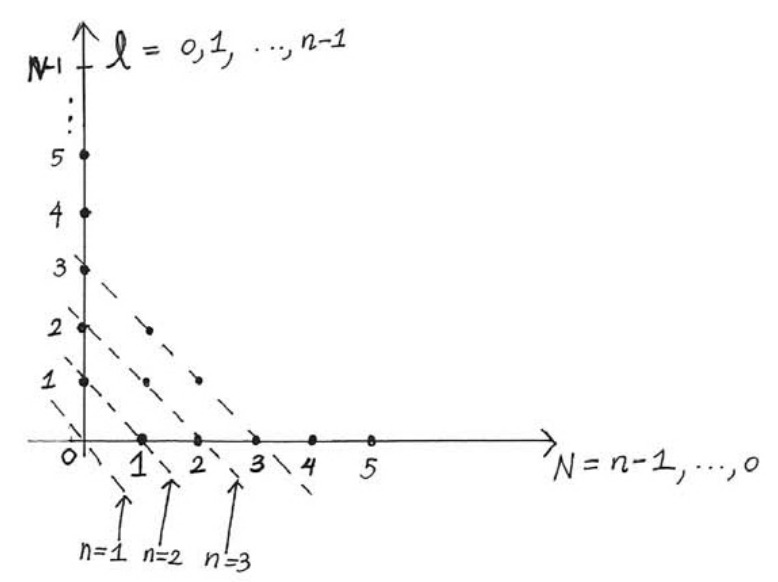
\includegraphics[width=0.5\linewidth]{resources/images/hydrogen_spectrum.png}
    \caption{A visualization of the spectrum of the hydrogen atom. States that share a dotted line are degenerate.}
    \label{hydrogen_spectrum}
\end{figure}

This figure helps us to count the number of bound states for a given value of $n$. Recall that $l$ can take values from $0$ to $n-1$, and for each value of $l$, the third quantum number $m$ can take the $(2l+1)$ values from $-l$ to $l$. Table \ref{hydrogen_spectrum} counts the states for the first three values of $n$. A state is specified by its values of $n$, $l$, and $m$, which are collectively referred to as the \textbf{quantum numbers} of the hydrogen atom. Each number has a very important physical meaning: $n$ specifies the energy eigenvalue, $\hbar^2 l(l+1)$ is the eigenvalue of the square of the angular momentum, and $\hbar m$ is the eigenvalue of the $z$-component of the angular momentum.

\begin{table}[]
    \centering
    \begin{tabular}{|c|c|c|c|}
    \hline
        $n$ & $l$ & $m$ & \# of states \\
        \hline
        $n=1$ & $l=1$ & $m=0$ & $1$ state \\
        \hline
        $n=2$ & $l=0$ & $m=1 $& $1$ \\
        & $l=1$ & $m=-1,0,1$ & $+3$ \\ 
        & & & $=4$ states \\
        \hline
        $n=3$ & $l=0$ & $m=0$ & $1$\\
        & $l=1$ & $m=-1,0,1$ & $+3$ \\
        & $l=2$ & $m=-2,\ldots,2$ & $+5$ \\
        & & & $=9$ states \\
    \hline
    \end{tabular}
    \caption{A table of the quantum numbers of the first few hydrogen atom eigenstates}
    \label{hydrogen_spectrum}
\end{table}

The total number of states for a given value of $n$ is $$\sum_{l=0}^{n-1}(2l+1)=\frac{2(n-1)n}{2}+n=n^2-n+n=n^2.$$Let us recap. Recall that way back at the beginning of our solution, we defined $\rho=\frac{2\kappa Z}{a_0}r$. But now we know what $\kappa$ is: $\kappa=\frac{1}{2n}$. This gives $$\rho=\frac{Z}{na_0}r.$$The wavefunctions are \begin{align*}\psi_{nlm}&=\mathcal{N}\frac{u_{nl}(r)}{r}Y_{lm}(\theta,\phi)=\mathcal{N}\frac{\rho^{l+1}}{\rho}W_{nl}(\rho)e^{-\rho}Y_{lm}(\theta,\phi)\\ &= \mathcal{N}\rho^l W_{nl}(\rho)e^{-\rho}Y_{lm}(\theta,\phi)\end{align*}where $\mathcal{N}$ is a normalization constant and $W_{nl}(\rho)$ is a polynomial of degree $N=n-l-1$. Substituting our expression for $\rho$ and absorbing constants into $N$, we have $$\boxed{\psi_{nlm}(r,\theta,\phi)=\mathcal{N}(\frac{r}{a_0})^l({\scriptstyle\text{polynomial in $\frac{r}{a_0}$ with degree $n-l-1$}})e^{-\frac{Zr}{na_0}}Y_{lm}(\theta,\phi)}.$$For the ground state of hydrogen, we have $Z=1$, $n=1$, $l=m=0$. Since there is no angular momentum, the associated wavefunction has no angular dependence. The normalized wavefunction is $$\psi_{100}(r,\theta,\phi)=\frac{1}{\sqrt{\pi a_0^3}}e^{-r/a_0}.$$For normalized wavefunctions of hydrogen with $n=1,2,3$, check out \href{http://hyperphysics.phy-astr.gsu.edu/hbase/quantum/hydwf.html}{this} website.

\begin{framedrmk*}
    What \textit{are} the mysterious polynomials $W_{nl}(\rho)$? They are known as the \textbf{associated Laguerre polynomials}, and more information about them can be found \href{https://en.wikipedia.org/wiki/Laguerre_polynomials#In_quantum_mechanics}{here}. They are quite interesting mathematical objects in their own right, but they are never necessary for any but the most precise calculations. 
\end{framedrmk*}

The canonical way of representing the energy levels of the hydrogen atom is shown in Figure \ref{hydrogen_energy_levels}. On the vertical axis we plot the possible values of $\frac{-1}{n^2}=\frac{2a_0E}{z^2e^2}$. Up to a proportionality constant, these represent the allowed energy levels. On the horizontal axis, we plot the possible values of $l$. 

\begin{figure}
    \centering
    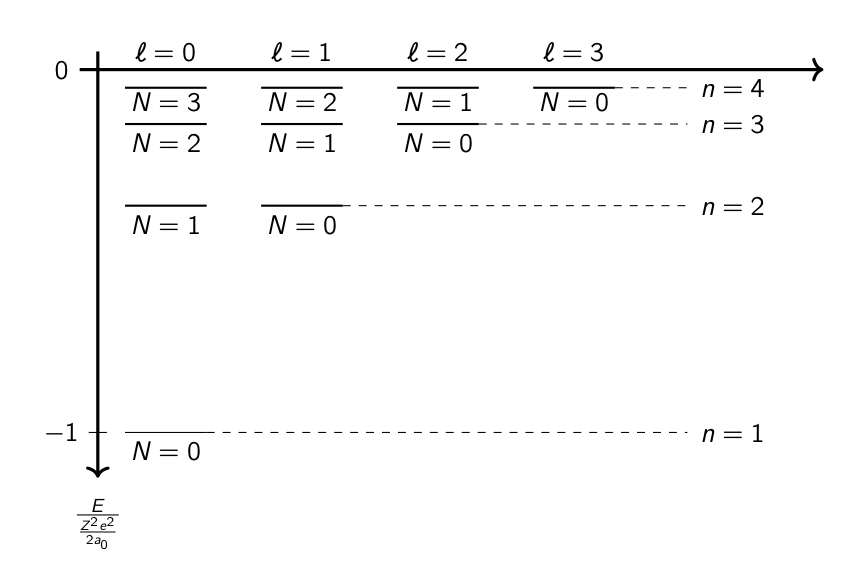
\includegraphics[width=0.5\linewidth]{resources/images/hydrogen_atom_energ_levels.png}
    \caption{A diagram of the energy levels of the hydrogen atom.}
    \label{hydrogen_energy_levels}
\end{figure}

As shown, the values of $N$ are constant along the diagonals, and increasing vertically. Why is this? Recall that for a constant value of $l$, the solutions obey a radial wave equation and thus the node theorem. Since all the nodes must come from the radial Laguerre polynomials, the polynomials must have degree increasing with $n$. Thus, $N$ must increase with $n$ to allow for more roots.

\subsection{Features of the Solutions}\label{features_of_the_solution}

It is important to note the extraordinary degeneracy within the hydrogen atom eigenstates. It is entirely unclear why $N=0$ eigenstates, for example, would be degenerate with $N=1$ eigenstates. In fact, the seemingly more simple system of the infinite spherical well has no degeneracies. The repeated eigenvalues of the hydrogen atom are a hint at a deeper symmetry that we are not yet aware of. We will explore this hidden symmetry in the coming sections.

We begin by rewriting the ground state wavefunction for the hydrogen atom, with $Z=1$ protons: $$\psi_{100}=\frac{1}{\sqrt{\pi a_0^3}}e^{-{r/a_0}}.$$We may ask how this wavefunction would change for $Z\neq 1$. Recall that the potential is $V(r)=-\frac{ze^2}{r}$. Then if $e^2$ becomes $Ze^2$, we can reason that $a_0=\frac{\hbar}{me^2}$ would become $\frac{a_0}{Z}$. Recall that $$E=-\frac{Z^2e^2}{2a_0}\frac{1}{n^2}.$$We can now see that one factor of $Z$ arises from the $e^2$ in the numerator, and the other factor is due to the $a_0$ in the denominator.

The general ground state wavefunction for an atom with $Z$ protons then becomes $$\psi_{100}=\sqrt{\frac{Z^3}{\pi a_0^3}}e^{-\frac{Zr}{a_0}}.$$We might also ask about the reason for the exponential $e^{-\frac{Zr}{na_0}}$ in the expression for the wavefunctions. Recall that we obtain the limiting case $$\frac{d^2u}{dr^2}=-\frac{2mE}{\hbar^2}u.$$The energy levels obey $$E_n=-\frac{Z^2e^2}{2a_0}\frac{1}{n^2}=-\frac{Z^2}{2a_0}\frac{\hbar^2}{ma_0}\frac{1}{n^2}.$$Therefore, $$-\frac{2mE_n}{\hbar^2}=\frac{Z^2}{n^2a_0^2}.$$Substituting, we have $$\frac{d^2u}{dr^2}=\frac{Z^2}{n^2a_0^2}u,$$which is solved by the exponential $$u(r)=e^{-\frac{Zr}{na_0}}.$$

\subsection{Rydberg Atoms}\label{rydberg_atoms}

A \textbf{Rydberg atom} is one in which one or more electrons is in a very high energy state. This leads to several unique properties. The outermost electron feels the attractive field due to the positive charge $Ze$ of the protons, but also the repulsive field due to the negative charge $(Z-1)e$ of the other electrons. Thus in any Rydberg atom, the outermost electron behaves as an electron in a hydrogen atom. One interesting question is the size (expected radius) of a Rydberg atom. To consider this, we state the \textbf{virial theorem}, an important result from statistical mechanics.

\begin{framedthm}[Virial theorem]
    For any particle in a potential $V$ with kinetic energy $T$, it is always true that $\langle T\rangle = -\frac{1}{2}\langle V\rangle$. In other words, $E=-\langle T\rangle$ and $\langle V\rangle=2E$.
\end{framedthm}

For a Rydberg atom (where we consider $Z=1$), the virial theorem gives $$\langle -\frac{e^2}{r}\rangle=2(-\frac{e^2}{2a_0}\frac{1}{n}).$$Simplifying, $$\langle\frac{1}{r}\rangle=\frac{1}{n^2 a_0}.$$Of course, the expectation value of $r$ is not the same as the reciprocal of the expected value of $\frac{1}{r}$. Instead, it turns out to be $$\langle r\rangle= n^2a_0[1+\frac{1}{2}(1-\frac{l(l+1)}{n^2})].$$Thus we see that the expected radius of a Rydberg atom does depend on $l$, but only very weakly. For $l=0$, we have $\langle r\rangle=\frac{3}{2}n^2a_0$, while for $l\to\infty$, we have $\langle r\rangle\approx n^2a_0$. 

Recall that the wavefunctions of the hydrogen atom are $$\psi_{nlm} = \mathcal{N}r^l W_{nl}(r)e^{-\frac{r}{na_0}}Y_{lm}(\theta,\phi)=f_{nl}(r)Y_{lm}(\Omega).$$We see that the exponential possesses a characteristic radius of $na_0$. Why is it, therefore, that the actual expected radius increases with $n^2$? We know that the probability $P(r)$ of finding the electron at a radius $r$ obeys $$P(r)dr=d^3x\,|\psi|^2=r^2dr\int d\Omega\,|\psi|^2=r^2dr\,|f_{nl}|^2\int d\Omega\,Y_{lm}^*Y_{lm}.$$The spherical harmonics are normalized, so we simply get $$P(r)=r^2|f_{nl}|^2.$$Let's expand $$f_{nl}(r)\sim r^l(a_0+\ldots+a'r^{n-l-1})e^{-r/na_0}.$$Since we're considering.a Rydberg atom, we can reason that the radius will be reasonably large. Thus, we keep only the term with highest degree in $r$: $$f_{nl}(r)\sim r^{n-1}e^{-r/na_0}.$$Therefore, the radial probability distribution obeys$$P(r)\sim r^{2n}e^{-\frac{2r}{na_0}}.$$We can see that there is a fight between an exponential with a characteristic width proportional to $na_0$, and a polynomial whose growth rate is dependent on $n$. We can find the maximum of this distribution by taking the derivative and setting it to $0$: $$(\frac{2n}{r}-\frac{2}{na_0})r^{2n}e^{-\frac{2r}{na_0}}=0.$$This implies that $\frac{2n}{r}=\frac{2}{na_0}$, which is solved when $$r=n^2a_0.$$Thus, the behavior of the probability distribution is directly dependent on $n^2$, not $n$. 

Interstellar hydrogen atoms can have immense energies; astrophysicists have observed electrons with $n$ as large as $350$! Using the expression we found above, we would expect such an atom to have radius $$r=a_0(350)^2=(0.53\times 10^{-10}\,\text{m})(350)^2\approx 6.5\,\mu\text{m}.$$This is an enormous atom! For contrast, a red blood cell has radius $8\mu\text{m}$. However, they do not decay as quickly as you might think. Energy levels characterized by $\frac{1}{n^2}$ have differences proportional to $\frac{1}{n^3}$. There are a lot of energy levels close together! Decaying from each to the next takes the atom up to a second.

\section{Degeneracies of the Hydrogen Atom}
\subsection{Hydrogen Atom Orbits}\label{hydrogen_orbits}

Consider an electron with $l=0$, and another electron with $l=99$. Which electron would have the most circular orbit? Although we often associate low $l$ with circular orbits, the $l=0$ electron actually has the most elliptical orbit, and the $l=99$ electron is the most circular. Why is this? Recall that the effective potential of the electron is $$\frac{\hbar l(l+1)}{2mr^2}-\frac{e^2}{r}.$$If $l=0$, the potential goes purely with $-\frac{1}{r}$. Classically,  the electron's radius would oscillate between $r=0$ and some maximum value $r'$. However, this is the definition of the most eccentric orbit!

As $l$ increases, the graphs of the potential have higher and higher minima, as shown in Figure \ref{hydrogen_potential_graph}. At some point, the minimum of the potential lies exactly on the energy of the electron. This corresponds to an orbit with fixed orbit --- a circle. 

\begin{figure}
    \centering
    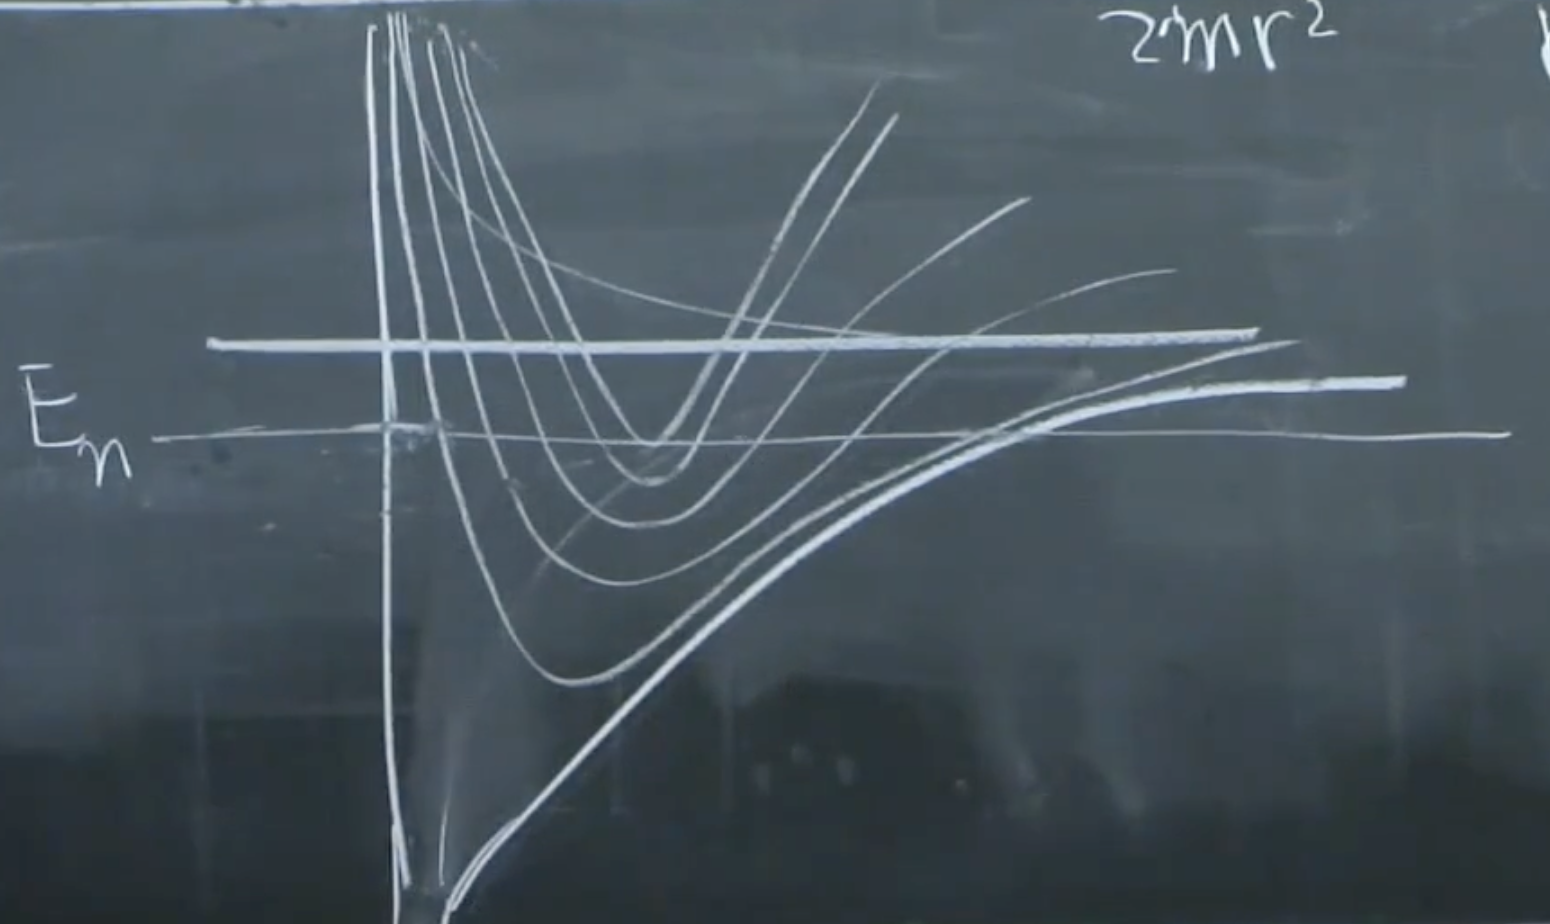
\includegraphics[width=0.5\linewidth]{resources/images/hydrogen_potential_graph.png}
    \caption{A graph of the potentials $V(r)$ for the hydrogen atom with differing values of $l$. As $l$ increases, the potentials have higher and higher minima.}
    \label{hydrogen_potential_graph}
\end{figure}

For any lower value of $l$, there exist two intersections between the effective potential and the energy value of the electron. These correspond to the two turning points of radius $r_-$ and $r_+$, respectively, as shown in Figure \ref{turning_points}. 

\begin{figure}
    \centering
    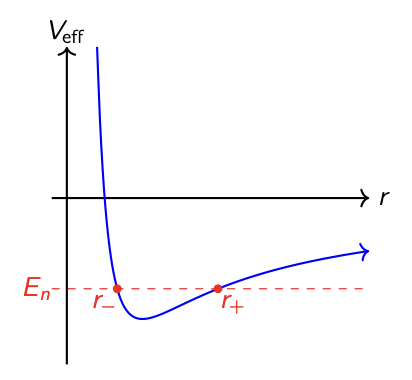
\includegraphics[width=0.5\linewidth]{resources/images/turning_points.png}
    \caption{A graph of the potential for some value of $l$. The two marked points are the turning points of radius $r_-$ and $r_+$, respectively.}
    \label{turning_points}
\end{figure}

\subsection{Turning Points}\label{turning_points_section}

We now solve explicitly for $r_-$ and $r_+$. We have $$V_{\text{eff}}(r)=\frac{\hbar^2 l(l+1)}{2mr^2}-\frac{e^2}{r}=E_n=-\frac{e^2}{2a_0}\frac{1}{n^2}$$at these turning points. We let $r=a_0x$, where $x$ is a unitfree length variable. This yields $$\frac{\hbar^2l(l+1)}{2ma_0^2}\frac{1}{x^2}-\frac{e^2}{a_0x}=-\frac{e^2}{2a_0}\frac{1}{n^2}.$$Also recall that $a_0=\frac{\hbar^2}{me^2}$, which gives $$\frac{\hbar^2}{2ma_0^2}=\frac{e^2}{2a_0}.$$Substituting, $$\frac{l(l+1)}{2a_0}\frac{1}{x^2}-\frac{e^2}{a_0x}=-\frac{e^2}{2a_0}\frac{1}{n}.$$Simplifying, $$\boxed{\frac{l(l+1)}{x^2}-\frac{2}{x}+\frac{1}{n^2}=0}.$$This is a quadratic in $\frac{1}{x}$. Multiplying both sides by $x^2$ gives us a quadratic in $x$. Solving, we get $$x=n^2\bigg(1\pm\sqrt{1-\frac{l(l+1)}{n^2}}\bigg).$$This yields $$r_\pm=n^2a_0\bigg(1\pm\sqrt{1-\frac{l(l+1)}{n^2}}\bigg).$$Recall that $l$ ranges from $0$ to $n$. When $l$ is very small, the orbit is extremely elliptical, as $r_\pm\approx n^2a_0(1\pm1)$. On the other hand, if $l$ is very large, the orbit is approximately circular: $r_\pm\approx n^2a_0$. Regardless of $l$, we see that $$\frac{1}{2}(r_-+r_+)=n^2a_0.$$

\begin{framedexpl}[Rydberg atom with $n=100$ and $l=60$]
    For $n=100$ and $l=60$, we have $r_+=18000a_0$, $r_-=2000a_0$.

\end{framedexpl}

Since the length of the semimajor axis of the orbit depends only on $n$, Kepler's third law tells us orbits with equal $n$ have equal periods. We know that periods are related to frequencies and thus energies, which explains why quantum states with equal $n$ are degenerate.

Lastly, consider a particular state with $l=1$. Then there are actually 3 degenerate states with this property: $m=-1$, $m=0$, and $m=1$. We don't represent these in our figures, but it should be noted that these degeneracies are always underlying.

    \chapter{Toward Matrix Mechanics}
    \section{The Simplest Quantum System}
\subsection{Wavefunctions as Vectors}\label{wavefunctions_as_vectors}

In the concluding thoughts of this course, we consider what the ``simplest'' quantum system is. Your first thought might be the particle in a box or the harmonic oscillator, but both have infinitely many bound states. In this sense, they are not very simple! Even the delta potential, which has only one bound state, has infinitely many scattering states. To find the \textit{simplest} quantum system, we go back to our roots.

We rewrite the Schrödinger equation: $$i\hbar\frac{\partial\Psi}{\partial t}=\hat{H}\Psi,$$which yields stationary states of the form $$\Psi=e^{-\frac{iEt}{\hbar}}\psi,$$where $\hat{H}\psi=E\psi$. Now, $\hat{H}$ can basically be \textit{whatever we want}, given that it is Hermitian: $\hat{H}^\dagger=\hat{H}$. 

In this course, we've solved the Schrödinger equation for a variety of potentials in $1$ and $3$ dimensions. To find the simplest quantum system, let's solve it in $0$ dimensions --- we restrict the particle to only $2$ possible points: $x_1$ and $x_2$. Instead of considering a continuous wavefunction $\psi(x)$, we now consider a \textit{vector} $$\begin{pmatrix} \psi(x_1) \\ \psi(x_2) \end{pmatrix}=\begin{pmatrix} \alpha \\ \beta \end{pmatrix},$$where $|\alpha|^2$ is the probability that the particle is at $x_1$, while $|\beta|^2$ is the probability that the particle is at $x_2$. This should remind you of our work with Mach-Zehnder interferometers at the very beginning of this course!

Now let's give our system some physical intuition. Maybe we have a box with two halves, and we wish to model the probability that the particle is on the left side of the box. Or maybe we have a particle with \textit{spin}, which can be either \textbf{spin up} or \textbf{spin down}. There are numerous cases in which a particle may be in only one of two states.

In a system with only two states, the inner product of two wavefunctions $\psi_1={\alpha_1\choose\beta_1}$ and $\psi_2={\alpha_2\choose\beta_2}$ is $$(\psi_1,\psi_2)=\alpha_1^*\alpha_2+\beta_1^*\beta_2=(\alpha_1^*\;\;\beta_1^*){\alpha_1\choose\beta_1}.$$In more advanced quantum mechanics, we represent \textit{continuous} wavefunctions in this way --- column vectors representing their values at all real points. In this language, a hermitian operator is a matrix $H$ such that $$(H^T)^*=H.$$

\subsection{Hamiltonians as Matrices}\label{hamiltonians_as_matrices}

Our wavefunctions have now been reduced to vectors in $2$ dimensions. Then the Hamiltonian is a $2\times2$ matrix, with the condition that $(H^T)^*=H$. This forces the diagonal elements to be real. The other elements can be complex. The most general form of a $2\times2$ Hermitian matrix is $$H=\begin{pmatrix}a_0+a_3 & a_1-ia_2 \\ a_1+ia_2 & a_0-a_3\end{pmatrix},$$where $a_0,a_1,a_2,a_3\in\mathbb{R}$. Notice that this indeed satisfies $(H^T)^*=H$. We can then decompose $H$ into its components: $$H=a_0\begin{pmatrix}1&0\\0&1\end{pmatrix}+a_1\begin{pmatrix}0&1\\1&0\end{pmatrix}+a_2\begin{pmatrix}0&-1\\i&0\end{pmatrix}+a_3\begin{pmatrix}1&0\\0&-1\end{pmatrix}.$$These four matrices form a basis of the set of all $2\times 2$ Hermitian matrices. They are so famous that the second, third, and fourth are given the special name of \textbf{Pauli matrices} and are denoted $\sigma_1$, $\sigma_2$, and $\sigma_3$. The first matrix is, of course, simply the identity $I$.

\begin{frameddefn}[Pauli matrices]
    The \textbf{Pauli matrices} form a basis of all $2\times2$ Hermitian matrices and are defined as follows: $$\sigma_1=\begin{pmatrix}0&1\\1&0\end{pmatrix},\quad\sigma_2=\begin{pmatrix}0&1\\1&0\end{pmatrix},\quad\sigma_3=\begin{pmatrix}1&0\\0&-1\end{pmatrix}.$$
\end{frameddefn}

Now, the Hamiltonian is not just any Hermitian matrix --- it must have units of energy. Thus we can write $$H=\frac{\hbar\omega_1}{2}\sigma_1+\frac{\hbar\omega_2}{2}\sigma_2+\frac{\hbar\omega_3}{2}\sigma_3,$$where the $\omega_i$ are some variables with units of angular frequency.

\begin{framedrmk*}[Identity matrix]
    Why don't we use the identity matrix $I$ in the Hamiltonian? Because adding $I$ to the Hamiltonian matrix corresponds to adding a scalar constant to the Hamiltonian operator, which we have already seen does nothing to the solutions. Instead, it merely changes how we define the zero-energy point. 
\end{framedrmk*}

We can rewrite the Hamiltonian $$H=\omega_1(\frac{\hbar}{2}\sigma_1)+\omega_2(\frac{\hbar}{2}\sigma_2)+\omega_3(\frac{\hbar}{2}\sigma_3).$$The terms in the parentheses have units of angular momentum. We see that in general, there can be three different angular momenta --- let's call them $S_x=\frac{\hbar}{2}\sigma_1$, $S_y=\frac{\hbar}{2}\sigma_2$, and $S_z=\frac{\hbar}{2}\sigma_3$. Note that these $S_i$ are all matrices. We can therefore find their commutators.

We write $$[S_x,S_y]=[\frac{\hbar}{2}\sigma_1,\frac{\hbar}{2}\sigma_2]=\frac{\hbar^2}{4}(\sigma_1\sigma_2-\sigma_2\sigma_1).$$Computing the matrix products gives $$[S_x,S_y]=i\hbar\,\frac{\hbar}{2}\begin{pmatrix}1&0 \\ 0 & -1\end{pmatrix}=i\hbar S_z.$$The analogous commutation relations are true for the other pairs. These matrices not only have the same units as angular momentum, but also behave identically to the angular momentum operators! 

\begin{framedrmk*}[Spin $\frac{1}{2}$]
    We have just discovered the basic properties of spin. Specifically, these matrices describe the spin of \textbf{spin-$\mathbf{\frac{1}{2}}$ particles}. All known \textbf{fermions}, which includes all particles that constitute matter, have spin $\frac{1}{2}$.
\end{framedrmk*}

\begin{framedrmk*}[NMR]
    Similarly to angular momentum, we can express the total spin as a vector operator $\hat{\mathbf{S}}$. We can then write $H=\vec{\omega}\,\mathbf{S}$. If we solve the equations governing spin in three dimensions, we find that spin precesses, just like angular momentum. This is the basis of \textbf{nuclear magnetic resonance}, or NMR.
\end{framedrmk*}

\subsection{Eigenstates as Eigenvectors}\label{eigenstates_as_eigenvectors}

We now proceed to find the eigenstates of each spin angular momentum operator. We have $$S_z=\frac{\hbar}{2}\begin{pmatrix}1 & 0 \\ 0 & -1\end{pmatrix}.$$It is already diagonalized, so the eigenstates are simply $1\choose0$ and $0\choose1$. We call the first state \textbf{spin up} and denote it $|\uparrow\rangle$, and we call the second state \textbf{spin down}, denoted $|\downarrow\rangle$. We have $S_z|\uparrow\rangle=\frac{\hbar}{2}|\uparrow\rangle$, and $S_z|\downarrow\rangle=-\frac{\hbar}{2}|\downarrow\rangle$. This system has spin $\frac{1}{2}$ because of the $\frac{1}{2}$ factor in the eigenvalues of $S_z$.

Next we write $$S_x=\frac{\hbar}{2}\begin{pmatrix}0 & 1 \\ 1 & 0\end{pmatrix}.$$Consider the state $$\frac{1}{\sqrt{2}}{1\choose1}=\frac{1}{\sqrt{2}}(|\uparrow\rangle+|\downarrow\rangle).$$What does $S_x$ do to this state? We have $$S_x\frac{1}{\sqrt{2}}{1\choose1}=\frac{\hbar}{2}\frac{1}{\sqrt{2}}\begin{pmatrix}0 & 1 \\ 1 & 0\end{pmatrix}{1\choose1}=\frac{\hbar}{2}\frac{1}{\sqrt{2}}{1\choose1}.$$Thus, this state is an eigenstate of $S_x$! We define it to be the spin up state in the $x$-direction and denote it $|\uparrow;\,x\rangle$. We similarly define the spin down state in the $x$-direction $|\downarrow;\,x\rangle=\frac{1}{\sqrt{2}}{1\choose -1}$.

Now we've gotten spin states along $x$ and $z$. What about $y$? There's one more thing to try: a \textit{complex} superposition$$\frac{1}{\sqrt{2}}{1\choose i}=\frac{1}{\sqrt{2}}(|\uparrow\rangle+i|\downarrow\rangle).$$Applying $S_y$ to this state, we have $$S_y\frac{1}{\sqrt{2}}{1\choose i}=\frac{\hbar}{2}\begin{pmatrix}0 & -i \\ i & 0\end{pmatrix}\frac{1}{\sqrt{2}}{1\choose i}=\frac{\hbar}{2}\frac{1}{\sqrt{2}}{1\choose i}.$$This state is indeed an eigenstate of $S_y$! We define it to be the spin up state in the $y$-direction and denote it $|\uparrow;\,y\rangle$. Similarly, we define the spin down state in the $y$-direction $|\downarrow;\,y\rangle=\frac{1}{\sqrt{2}}{1\choose -i}$.

\subsection{Closing}

To conclude, what we have found here is that spin is an entirely different quantity from the position and momentum wavefunctions we've explored earlier in this course. The spin wavefunctions are simply $2$-dimensional vectors and are operated on by $2\times 2$ Hermitian matrices. Despite their simplicity, they are highly useful in modeling all sorts of quantum systems, including quantum computers and Bell experiments. 

Throughout this course, you have learned the fundamentals of quantum mechanics and even applied it to solve a problem as rich as the hydrogen atom. Take a moment to appreciate how far you've come! If you're like me, many of the concepts --- tunneling through a potential barrier, entanglement of two particles, nondeterminism --- might have seemed mystical before learning the theory behind them. I hope that seeing how these phenomena are consequences of something as familiar as calculus or linear algebra has made them much less formidable.

Quantum mechanics has been around for just around a century, and it is far from a completed field. Nonetheless, there is so much more to explore, from quantum computing to quantum chemistry, and you've laid a great foundation to continue building on. Regardless of where your future studies take you, I'd like to thank you again for taking the time to read my notes. Good luck, and godspeed.
    
\end{document}
